\hypertarget{sensation-receptors-organs-and-systems}{%
\chapter{Sensation: Receptors, Organs And Systems}\label{sensation-receptors-organs-and-systems}}

Sensation is the physical process during which sensory systems respond to stimuli and provide data for perception. A sense is any of the systems involved in sensation. During sensation, sense organs engage in stimulus collection and transduction. Sensation is often differentiated from the related and dependent concept of perception, which processes and integrates sensory information in order to give meaning to and understand detected stimuli, giving rise to subjective perceptual experience, or qualia. Sensation and perception are central to and precede almost all aspects of cognition, behavior and thought.

The sensory nervous system is a part of the nervous system responsible for processing sensory information. A sensory system consists of sensory neurons (including the sensory receptor cells), neural pathways, and parts of the brain involved in sensory perception. Commonly recognized sensory systems are those for vision, hearing, touch, taste, smell, and balance. In short, senses are transducers from the physical world to the realm of the mind where we interpret the information, creating our perception of the world around us.

Organisms need information to solve at least three kinds of problems: (a) to maintain an appropriate environment, i.e., homeostasis; (b) to time activities (e.g., seasonal changes in behavior) or synchronize activities with those of conspecifics; and (c) to locate and respond to resources or threats (e.g., by moving towards resources or evading or attacking threats). Organisms also need to transmit information in order to influence another's behavior: to identify themselves, warn conspecifics of danger, coordinate activities, or deceive.

The receptive field is the area of the body or environment to which a receptor organ and receptor cells respond. For instance, the part of the world an eye can see, is its receptive field; the light that each rod or cone can see, is its receptive field. Receptive fields have been identified for the visual system, auditory system and somatosensory system.

Sensory systems code for four aspects of a stimulus; type (modality), intensity, location, and duration. Arrival time of a sound pulse and phase differences of continuous sound are used for sound localization. Certain receptors are sensitive to certain types of stimuli (for example, different mechanoreceptors respond best to different kinds of touch stimuli, like sharp or blunt objects). Receptors send impulses in certain patterns to send information about the intensity of a stimulus (for example, how loud a sound is). The location of the receptor that is stimulated gives the brain information about the location of the stimulus (for example, stimulating a mechanoreceptor in a finger will send information to the brain about that finger). The duration of the stimulus (how long it lasts) is conveyed by firing patterns of receptors. These impulses are transmitted to the brain through afferent neurons.

While debate exists among neurologists as to the specific number of senses due to differing definitions of what constitutes a sense, Gautama Buddha and Aristotle classified five `traditional' human senses which have become universally accepted: touch, taste, smell, sight, and hearing. Other senses that have been well-accepted in most mammals, including humans, include nociception, equilibrioception, kinaesthesia, and thermoception. Furthermore, some nonhuman animals have been shown to possess alternate senses, including magnetoception and electroreception.

In organisms, a sensory organ consists of a group of related sensory cells that respond to a specific type of physical stimulus. Via cranial and spinal nerves, the different types of sensory receptor cells (mechanoreceptors, photoreceptors, chemoreceptors, thermoreceptors) in sensory organs transduct sensory information from sensory organs towards the central nervous system, to the sensory cortices in the brain, where sensory signals are further processed and interpreted (perceived). Sensory systems, or senses, are often divided into external (exteroception) and internal (interoception) sensory systems. Sensory modalities or submodalities refer to the way sensory information is encoded or transduced. Multimodality integrates different senses into one unified perceptual experience. For example, information from one sense has the potential to influence how information from another is perceived. Sensation and perception are studied by a variety of related fields, most notably psychophysics, neurobiology, cognitive psychology, and cognitive science.

Humans have a multitude of sensory systems. Human external sensation is based on the sensory organs of the eyes, ears, skin, inner ear, nose, and mouth. The corresponding sensory systems of the visual system (sense of vision), auditory system (sense of hearing), somatosensory system (sense of touch), vestibular system (sense of balance), olfactory system (sense of smell), and gustatory system (sense of taste) contribute, respectively, to the perceptions of vision, hearing, touch, spatial orientation, smell, and taste (flavor). Internal sensation, or interoception, detects stimuli from internal organs and tissues. Many internal sensory and perceptual systems exist in humans, including proprioception (body position) and nociception (pain). Further internal chemoreception and osmoreception based sensory systems lead to various perceptions, such as hunger, thirst, suffocation, and nausea, or different involuntary behaviors, such as vomiting.

Nonhuman animals experience sensation and perception, with varying levels of similarity to and difference from humans and other animal species. For example, mammals, in general, have a stronger sense of smell than humans. Some animal species lack one or more human sensory system analogues, some have sensory systems that are not found in humans, while others process and interpret the same sensory information in very different ways. For example, some animals are able to detect electrical and magnetic fields, air moisture, or polarized light, while others sense and perceive through alternative systems, such as echolocation. Recently, it has been suggested that plants and artificial agents may be able to detect and interpret environmental information in an analogous manner to animals.

\hypertarget{sensory-receptors}{%
\section{Sensory Receptors}\label{sensory-receptors}}

Sensory receptors are the cells or structures that detect sensations. Stimuli in the environment activate specialized receptor cells in the peripheral nervous system. During transduction, physical stimulus is converted into action potential by receptors and transmitted towards the central nervous system for processing. Different types of stimuli are sensed by different types of receptor cells. Receptor cells can be classified into types on the basis of three different criteria: cell type, position, and function. Receptors can be classified structurally on the basis of cell type and their position in relation to stimuli they sense. Receptors can further be classified functionally on the basis of the transduction of stimuli, or how the mechanical stimulus, light, or chemical changed the cell membrane potential.

One way to classify receptors is based on their location relative to the stimuli. An exteroceptor is a receptor that is located near a stimulus of the external environment, such as the somatosensory receptors that are located in the skin. An interoceptor is one that interprets stimuli from internal organs and tissues, such as the receptors that sense the increase in blood pressure in the aorta or carotid sinus.

The cells that interpret information about the environment can be either (1) a neuron that has a free nerve ending, with dendrites embedded in tissue that would receive a sensation; (2) a neuron that has an encapsulated ending in which the sensory nerve endings are encapsulated in connective tissue that enhances their sensitivity; or (3) a specialized receptor cell, which has distinct structural components that interpret a specific type of stimulus. The pain and temperature receptors in the dermis of the skin are examples of neurons that have free nerve endings (1). Also located in the dermis of the skin are lamellated corpuscles, neurons with encapsulated nerve endings that respond to pressure and touch (2). The cells in the retina that respond to light stimuli are an example of a specialized receptor (3), a photoreceptor.

A transmembrane protein receptor is a protein in the cell membrane that mediates a physiological change in a neuron, most often through the opening of ion channels or changes in the cell signaling processes. Transmembrane receptors are activated by chemicals called ligands. For example, a molecule in food can serve as a ligand for taste receptors. Other transmembrane proteins, which are not accurately called receptors, are sensitive to mechanical or thermal changes. Physical changes in these proteins increase ion flow across the membrane, and can generate an action potential or a graded potential in the sensory neurons.

A third classification of receptors is by how the receptor transduces stimuli into membrane potential changes. Stimuli are of three general types. Some stimuli are ions and macromolecules that affect transmembrane receptor proteins when these chemicals diffuse across the cell membrane. Some stimuli are physical variations in the environment that affect receptor cell membrane potentials. Other stimuli include the electromagnetic radiation from visible light. For humans, the only electromagnetic energy that is perceived by our eyes is visible light. Some other organisms have receptors that humans lack, such as the heat sensors of snakes, the ultraviolet light sensors of bees, or magnetic receptors in migratory birds.

Receptor cells can be further categorized on the basis of the type of stimuli they transduce. The different types of functional receptor cell types are mechanoreceptors, photoreceptors, chemoreceptors (osmoreceptor), thermoreceptors, and nociceptors. Physical stimuli, such as pressure and vibration, as well as the sensation of sound and body position (balance), are interpreted through a mechanoreceptor. Photoreceptors convert light (visible electromagnetic radiation) into signals. Chemical stimuli can be interpreted by a chemoreceptor that interprets chemical stimuli, such as an object's taste or smell, while osmoreceptors respond to a chemical solute concentrations of body fluids. Nociception (pain) interprets the presence of tissue damage, from sensory information from mechano-, chemo-, and thermoreceptors. Another physical stimulus that has its own type of receptor is temperature, which is sensed through a thermoreceptor that is either sensitive to temperatures above (heat) or below (cold) normal body temperature.

Each sense organ (eyes or nose, for instance) requires a minimal amount of stimulation in order to detect a stimulus. This minimum amount of stimulus is called the absolute threshold. The absolute threshold is defined as the minimum amount of stimulation necessary for the detection of a stimulus 50\% of the time. Absolute threshold is measured by using a method called signal detection. This process involves presenting stimuli of varying intensities to a subject in order to determine the level at which the subject can reliably detect stimulation in a given sense.

Differential threshold or just noticeable difference (JDS) is the smallest detectable difference between two stimuli, or the smallest difference in stimuli that can be judged to be different from each other. Weber's Law is an empirical law that states that the difference threshold is a constant fraction of the comparison stimulus. According to Weber's Law, bigger stimuli require larger differences to be noticed.

Perception occurs when nerves that lead from the sensory organs (e.g.~eye) to the brain are stimulated, even if that stimulation is unrelated to the target signal of the sensory organ. For example, in the case of the eye, it does not matter whether light or something else stimulates the optic nerve, that stimulation will results in visual perception, even if there was no visual stimulus to begin with. (To prove this point to yourself (and if you are a human), close your eyes (preferably in a dark room) and press gently on the outside corner of one eye through the eyelid. You will see a visual spot toward the inside of your visual field, near your nose.

The initialization of sensation stems from the response of a specific receptor to a physical stimulus. The receptors which react to the stimulus and initiate the process of sensation are commonly characterized in four distinct categories: chemoreceptors, photoreceptors, mechanoreceptors, and thermoreceptors. All receptors receive distinct physical stimuli and transduce the signal into an electrical action potential. This action potential then travels along afferent neurons to specific brain regions where it is processed and interpreted.

\hypertarget{chemoreceptors}{%
\subsection{Chemoreceptors}\label{chemoreceptors}}

Chemoreceptors, or chemosensors, detect certain chemical stimuli and transduce that signal into an electrical action potential. The two primary types of chemoreceptors are:

Distance chemoreceptors are integral to receiving stimuli in gases in the olfactory system through both olfactory receptor neurons and neurons in the vomeronasal organ.
Direct chemoreceptors that detect stimuli in liquids include the taste buds in the gustatory system as well as receptors in the aortic bodies which detect changes in oxygen concentration.

\hypertarget{photoreceptors}{%
\subsection{Photoreceptors}\label{photoreceptors}}

Photoreceptors are capable of phototransduction, a process which converts light (electromagnetic radiation) into, among other types of energy, a membrane potential. The three primary types of photoreceptors are: Cones are photoreceptors which respond significantly to color. In humans the three different types of cones correspond with a primary response to short wavelength (blue), medium wavelength (green), and long wavelength (yellow/red). Rods are photoreceptors which are very sensitive to the intensity of light, allowing for vision in dim lighting. The concentrations and ratio of rods to cones is strongly correlated with whether an animal is diurnal or nocturnal. In humans rods outnumber cones by approximately 20:1, while in nocturnal animals, such as the tawny owl, the ratio is closer to 1000:1. Ganglion Cells reside in the adrenal medulla and retina where they are involved in the sympathetic response. Of the \textasciitilde1.3 million ganglion cells present in the retina, 1-2\% are believed to be photosensitive ganglia. These photosensitive ganglia play a role in conscious vision for some animals, and are believed to do the same in humans.

\hypertarget{mechanoreceptors}{%
\subsection{Mechanoreceptors}\label{mechanoreceptors}}

Mechanoreceptors are sensory receptors which respond to mechanical forces, such as pressure or distortion. While mechanoreceptors are present in hair cells and play an integral role in the vestibular and auditory systems, the majority of mechanoreceptors are cutaneous and are grouped into four categories:

\begin{itemize}
\tightlist
\item
  Slowly adapting type 1 receptors have small receptive fields and respond to static stimulation. These receptors are primarily used in the sensations of form and roughness.
\item
  Slowly adapting type 2 receptors have large receptive fields and respond to stretch. Similarly to type 1, they produce sustained responses to a continued stimuli.
\item
  Rapidly adapting receptors have small receptive fields and underlie the perception of slip.
  Pacinian receptors have large receptive fields and are the predominant receptors for high-frequency vibration.
\end{itemize}

\hypertarget{thermoreceptors}{%
\subsection{Thermoreceptors}\label{thermoreceptors}}

Thermoreceptors are sensory receptors which respond to varying temperatures. While the mechanisms through which these receptors operate is unclear, recent discoveries have shown that mammals have at least two distinct types of thermoreceptors:{[}permanent dead link{]}‹See TfM›{[}failed verification{]}

\begin{itemize}
\tightlist
\item
  The end-bulb of Krause, or bulboid corpuscle, detects temperatures above body temperature.
\item
  Ruffini's end organ detects temperatures below body temperature.
\end{itemize}

TRPV1 is a heat-activated channel that acts as a small heat detecting thermometer in the membrane which begins the polarization of the neural fiber when exposed to changes in temperature. Ultimately, this allows us to detect ambient temperature in the warm/hot range. Similarly, the molecular cousin to TRPV1, TRPM8, is a cold-activated ion channel that responds to cold. Both cold and hot receptors are segregated by distinct subpopulations of sensory nerve fibers, which shows us that the information coming into the spinal cord is originally separate. Each sensory receptor has its own ``labeled line'' to convey a simple sensation experienced by the recipient. Ultimately, TRP channels act as thermosensors, channels that help us to detect changes in ambient temperatures.

\hypertarget{nociceptors}{%
\subsection{Nociceptors}\label{nociceptors}}

Nociceptors respond to potentially damaging stimuli by sending signals to the spinal cord and brain. This process, called nociception, usually causes the perception of pain. They are found in internal organs, as well as on the surface of the body. Nociceptors detect different kinds of damaging stimuli or actual damage. Those that only respond when tissues are damaged are known as ``sleeping'' or ``silent'' nociceptors.

Thermal nociceptors are activated by noxious heat or cold at various temperatures.
Mechanical nociceptors respond to excess pressure or mechanical deformation.
Chemical nociceptors respond to a wide variety of chemicals, some of which are signs of tissue damage. They are involved in the detection of some spices in food.

\hypertarget{the-visual-system}{%
\section{The Visual System}\label{the-visual-system}}

Visual perception is the ability to interpret the surrounding environment using light in the visible spectrum reflected by the objects in the environment. This is different from visual acuity, which refers to how clearly a person sees (for example ``20/20 vision''). A person can have problems with visual perceptual processing even if they have 20/20 vision.

The resulting perception is also known as visual perception, eyesight, sight, or vision. The various physiological components involved in vision are referred to collectively as the visual system.

Different species are able to see different parts of the light spectrum; for example, bees can see into the ultraviolet, while pit vipers can accurately target prey with their pit organs, which are sensitive to infrared radiation. The mantis shrimp possesses arguably the most complex visual system in any species. The eye of the mantis shrimp holds 16 color receptive cones, whereas humans only have three. The variety of cones enables them to perceive an enhanced array of colors as a mechanism for mate selection, avoidance of predators, and detection of prey. Swordfish also possess an impressive visual system. The eye of a swordfish can generate heat to better cope with detecting their prey at depths of 2000 feet. Certain one-celled micro-organisms, the warnowiid dinoflagellates have eye-like ocelloids, with analogous structures for the lens and retina of the multi-cellular eye. The armored shell of the chiton \emph{Acanthopleura granulata} is also covered with hundreds of aragonite crystalline eyes, named ocelli, which can form images.

Many fan worms, such as \emph{Acromegalomma interruptum} which live in tubes on the sea floor of the Great Barrier Reef, have evolved compound eyes on their tentacles, which they use to detect encroaching movement. If movement is detected the fan worms will rapidly withdraw their tentacles.

Only higher primate Old World (African) monkeys and apes have the same kind of three-cone photoreceptor color vision humans have, while lower primate New World (South American) monkeys have a two-cone photoreceptor kind of color vision.

\hypertarget{the-eye}{%
\subsection{The Eye}\label{the-eye}}

Light entering the eye is refracted as it passes through the cornea. It then passes through the pupil (controlled by the iris) and is further refracted by the lens. The cornea and lens act together as a compound lens to project an inverted image onto the retina.



\begin{figure}

{\centering 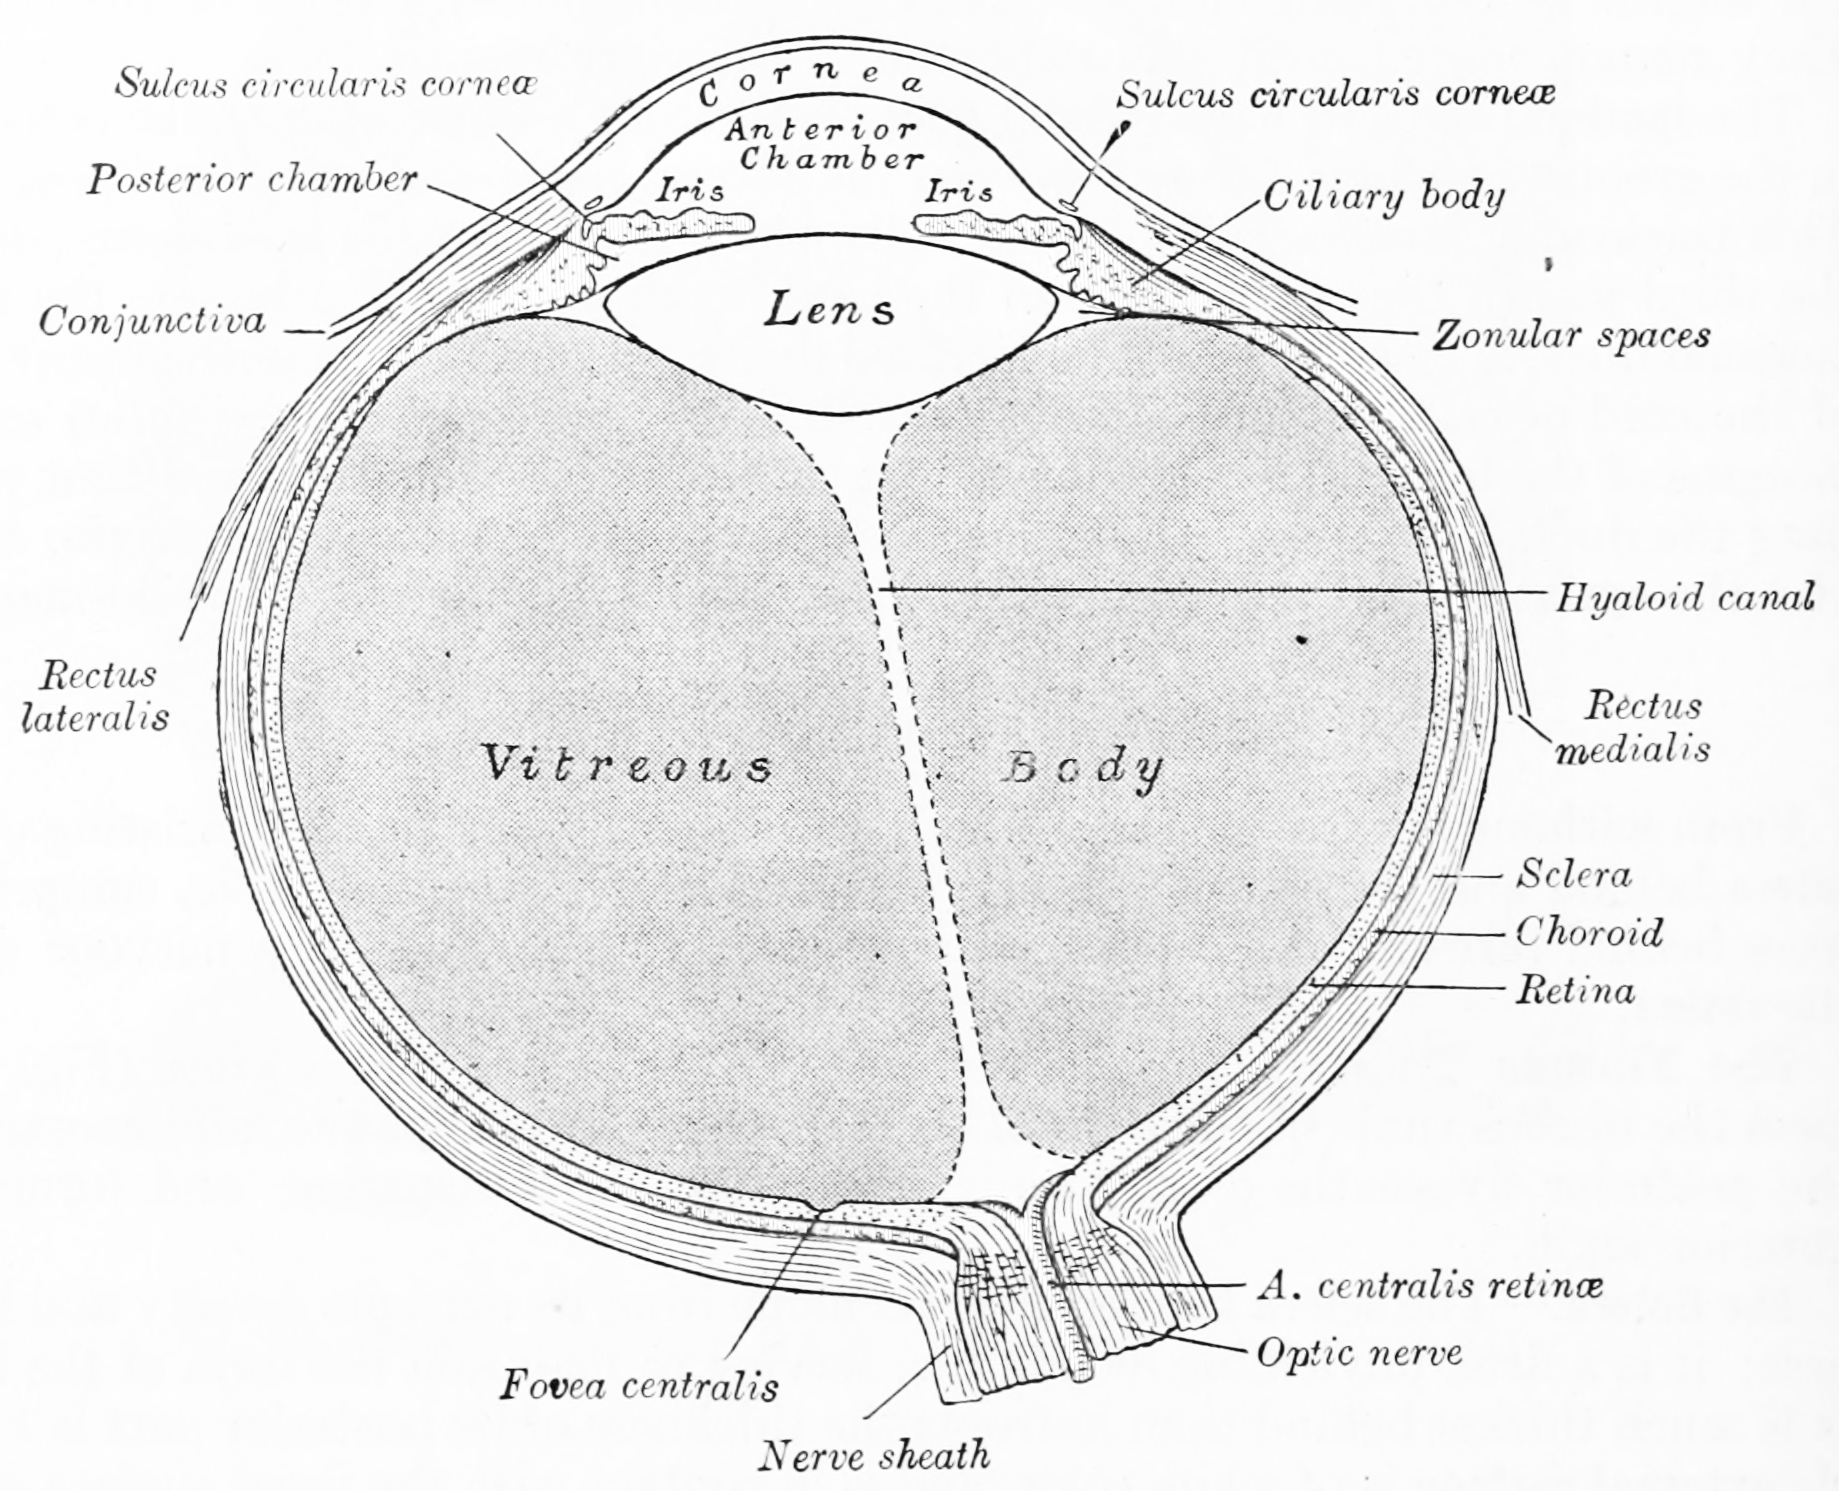
\includegraphics[width=0.7\linewidth]{./figures/sensation/anatomyofhumanbo1918gray_1008} 

}

\caption{Horizontal section of the human eyeball. From \href{https://archive.org/details/anatomyofhumanbo1918gray/page/n6/mode/2up}{Gray Henry, Anatomy of the Human Body. 20\textsuperscript{th} Edition, Lea \& Febiger, Philadelphia \& New York, 1918}}\label{fig:eye}
\end{figure}

\hypertarget{the-retina}{%
\subsection{The Retina}\label{the-retina}}

The retina is the light-sensitive layer of tissue of the eye of most vertebrates and some molluscs. The optics of the eye create a focused two-dimensional image of the visual world on the retina, which translates that image into electrical neural impulses to the brain to create visual perception.

The retina translates an optical image into neural impulses starting with the patterned excitation of the light-sensitive pigments of its rods and cones, the retina's photoreceptor cells. The excitation is processed by the neural system and various parts of the brain working in parallel to form a representation of the external environment in the brain.

Light striking the retina initiates a cascade of chemical and electrical events that ultimately trigger nerve impulses that are sent to various visual centres of the brain through the fibres of the optic nerve. Neural signals from the rods and cones undergo processing by other neurons, whose output takes the form of action potentials in retinal ganglion cells whose axons form the optic nerve. Several important features of visual perception can be traced to the retinal encoding and processing of light.

The cones respond to bright light and mediate high-resolution colour vision during daylight illumination (also called photopic vision). The rod responses are saturated at daylight levels and don't contribute to pattern vision. However, rods do respond to dim light and mediate lower-resolution, monochromatic vision under very low levels of illumination (called scotopic vision). The illumination in most office settings falls between these two levels and is called mesopic vision. At mesopic light levels, both the rods and cones are actively contributing pattern information. What contribution the rod information makes to pattern vision under these circumstances is unclear.

The response of cones to various wavelengths of light is called their spectral sensitivity. In normal human vision, the spectral sensitivity of a cone falls into one of three subtypes, often called blue, green, and red, but more accurately known as short, medium, and long wavelength-sensitive cone subtypes. It is a lack of one or more of the cone subtypes that causes individuals to have deficiencies in colour vision or various kinds of colour blindness. These individuals are not blind to objects of a particular colour, but are unable to distinguish between colours that can be distinguished by people with normal vision. Humans have this trichromatic vision, while most other mammals lack cones with red sensitive pigment and therefore have poorer dichromatic colour vision. However, some animals have four spectral subtypes, e.g.~the trout adds an ultraviolet subgroup to short, medium, and long subtypes that are similar to humans. Some fish are sensitive to the polarization of light as well.

When thus excited by light, the photoceptor sends a proportional response synaptically to bipolar cells which in turn signal the retinal ganglion cells. The photoreceptors are also cross-linked by horizontal cells and amacrine cells, which modify the synaptic signal before it reaches the ganglion cells, the neural signals being intermixed and combined. Of the retina's nerve cells, only the retinal ganglion cells and few amacrine cells create action potentials.

In the retinal ganglion cells there are two types of response, depending on the receptive field of the cell. The receptive fields of retinal ganglion cells comprise a central, approximately circular area, where light has one effect on the firing of the cell, and an annular surround, where light has the opposite effect. In ON cells, an increment in light intensity in the centre of the receptive field causes the firing rate to increase. In OFF cells, it makes it decrease. Beyond this simple difference, ganglion cells are also differentiated by chromatic sensitivity and the type of spatial summation. Cells showing linear spatial summation are termed X cells (also called parvocellular, P, or midget ganglion cells), and those showing non-linear summation are Y cells (also called magnocellular, M, or parasol retinal ganglion cells), although the correspondence between X and Y cells (in the cat retina) and P and M cells (in the primate retina) is not as simple as it once seemed.

In the transfer of visual signals to the brain, the visual pathway, the retina is vertically divided in two, a temporal (nearer to the temple) half and a nasal (nearer to the nose) half. The axons from the nasal half cross the brain at the optic chiasma to join with axons from the temporal half of the other eye before passing into the lateral geniculate body.

Although there are more than 130 million retinal receptors, there are only approximately 1.2 million fibres (axons) in the optic nerve. So, a large amount of pre-processing is performed within the retina. The fovea produces the most accurate information. Despite occupying about 0.01\% of the visual field (less than 2° of visual angle), about 10\% of axons in the optic nerve are devoted to the fovea.

The final result of all this processing is five different populations of ganglion cells that send visual (image-forming and non-image-forming) information to the brain:

\begin{itemize}
\tightlist
\item
  M cells, with large center-surround receptive fields that are sensitive to depth, indifferent to color, and rapidly adapt to a stimulus
\item
  P cells, with smaller center-surround receptive fields that are sensitive to color and shape
\item
  K cells, with very large center-only receptive fields that are sensitive to color and indifferent to shape or depth
\item
  another population that is intrinsically photosensitive
\item
  a final population that is involved in the control of eye movements.
  The neural retina consists of several layers of neurons interconnected by synapses, and is supported by an outer layer of pigmented epithelial cells. The primary light-sensing cells in the retina are the photoreceptor cells, which are of two types: rods and cones. Rods function mainly in dim light and provide black-and-white vision. Cones function in well-lit conditions and are responsible for the perception of colour, as well as high-acuity vision used for tasks such as reading. A third type of light-sensing cell, the photosensitive ganglion cell, is important for entrainment of circadian rhythms and reflexive responses such as the pupillary light reflex.
\end{itemize}

In vertebrate embryonic development, the retina and the optic nerve originate as outgrowths of the developing brain, specifically the embryonic diencephalon; thus, the retina is considered part of the central nervous system (CNS) and is actually brain tissue. It is the only part of the CNS that can be visualized non-invasively.

The vertebrate retina has ten distinct layers. From closest to farthest from the vitreous body:

\begin{itemize}
\tightlist
\item
  Inner limiting membrane -- basement membrane elaborated by Müller cells.
\item
  Nerve fibre layer -- axons of the ganglion cell bodies (note that a thin layer of Müller cell footplates exists between this layer and the inner limiting membrane).
\item
  Ganglion cell layer -- contains nuclei of ganglion cells, the axons of which become the optic nerve fibres, and some displaced amacrine cells.
\item
  Inner plexiform layer -- contains the synapse between the bipolar cell axons and the dendrites of the ganglion and amacrine cells.
\item
  Inner nuclear layer -- contains the nuclei and surrounding cell bodies (perikarya) of the amacrine cells, bipolar cells, and horizontal cells.
\item
  Outer plexiform layer -- projections of rods and cones ending in the rod spherule and cone pedicle, respectively. These make synapses with dendrites of bipolar cells and horizontal cells. In the macular region, this is known as the Fiber layer of Henle.
\item
  Outer nuclear layer -- cell bodies of rods and cones.
\item
  External limiting membrane -- layer that separates the inner segment portions of the photoreceptors from their cell nuclei.
\item
  Inner segment / outer segment layer -- inner segments and outer segments of rods and cones. The outer segments contain a highly specialized light-sensing apparatus.
\item
  Retinal pigment epithelium -- single layer of cuboidal epithelial cells. This layer is closest to the choroid, and provides nourishment and supportive functions to the neural retina, The black pigment melanin in the pigment layer prevents light reflection throughout the globe of the eyeball.
\end{itemize}

These layers can be grouped into 4 main processing stages: photoreception; transmission to bipolar cells; transmission to ganglion cells, which also contain photoreceptors, the photosensitive ganglion cells; and transmission along the optic nerve. At each synaptic stage there are also laterally connecting horizontal and amacrine cells.



\begin{figure}

{\centering 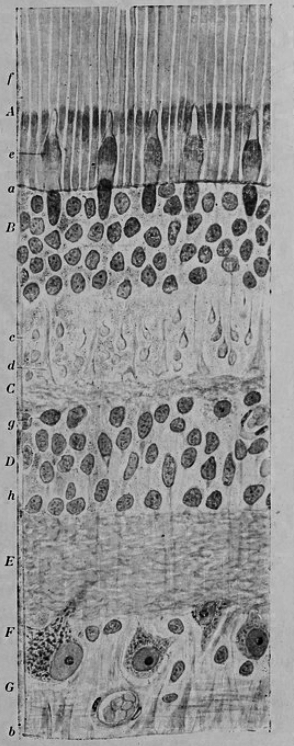
\includegraphics[width=0.7\linewidth]{./figures/sensation/retina_cajal} 

}

\caption{Vertical section of the adult human retina. Carmine and Nissl stain. \emph{A}, Photoreceptor layer. \emph{B}, Cell bodies of the photoreceptors. \emph{C}, Outer plexiform layer. \emph{D}, Internal granule layer. \emph{E}, Internal plexiform layer. \emph{F}, Ganglion cell layer. \emph{G}, Ganglion cell axons. \emph{a}, external limiting membrane. \emph{b}, internal limiting membrane. \emph{c}, Spherical endfeet of the rod photoreceptors. \emph{d}, endfeet of the cones. e. \emph{a}, cone. \emph{f}, a rod \emph{g}, horizontal cells. \emph{h}, amacrine cells. Fig. 188 from \href{https://wellcomelibrary.org/item/b2129592x\#?c=0\&m=0\&s=0\&cv=0\&z=-0.9137\%2C-0.0887\%2C2.8274\%2C1.7747}{Histologie du système nerveux de l'homme \& des vertébrés} (1909) by Santiago Ramón y Cajal translated from Spanish by Dr.~L. Azoulay.}\label{fig:retcajal}
\end{figure}

The optic nerve is a central tract of many axons of ganglion cells connecting primarily to the lateral geniculate body, a visual relay station in the diencephalon (the rear of the forebrain). It also projects to the superior colliculus, the suprachiasmatic nucleus, and the nucleus of the optic tract. It passes through the other layers, creating the optic disc in primates.

Additional structures, not directly associated with vision, are found as outgrowths of the retina in some vertebrate groups. In birds, the pecten is a vascular structure of complex shape that projects from the retina into the vitreous humour; it supplies oxygen and nutrients to the eye, and may also aid in vision. Reptiles have a similar, but much simpler, structure.

In adult humans, the entire retina is approximately 72\% of a sphere about 22 mm in diameter. The entire retina contains about 7 million cones and 75 to 150 million rods. The optic disc, a part of the retina sometimes called ``the blind spot'' because it lacks photoreceptors, is located at the optic papilla, where the optic-nerve fibres leave the eye. It appears as an oval white area of 3 mm². Temporal (in the direction of the temples) to this disc is the macula, at whose centre is the fovea, a pit that is responsible for our sharp central vision but is actually less sensitive to light because of its lack of rods. Human and non-human primates possess one fovea, as opposed to certain bird species, such as hawks, who are bifoviate, and dogs and cats, who possess no fovea but a central band known as the visual streak. Around the fovea extends the central retina for about 6 mm and then the peripheral retina. The farthest edge of the retina is defined by the ora serrata.

In section, the retina is no more than 0.5 mm thick. It has three layers of nerve cells and two of synapses, including the unique ribbon synapse. The optic nerve carries the ganglion cell axons to the brain, and the blood vessels that supply the retina. The ganglion cells lie innermost in the eye while the photoreceptive cells lie beyond. Because of this counter-intuitive arrangement, light must first pass through and around the ganglion cells and through the thickness of the retina, before reaching the rods and cones. Light is absorbed by the retinal pigment epithelium or the choroid.

The white blood cells in the capillaries in front of the photoreceptors can be perceived as tiny bright moving dots when looking into blue light. This is known as the blue field entoptic phenomenon (or Scheerer's phenomenon).

Between the ganglion cell layer and the rods and cones there are two layers of neuropils where synaptic contacts are made. The neuropil layers are the outer plexiform layer and the inner plexiform layer. In the outer neuropil layer, the rods and cones connect to the vertically running bipolar cells, and the horizontally oriented horizontal cells connect to ganglion cells.



\begin{figure}

{\centering 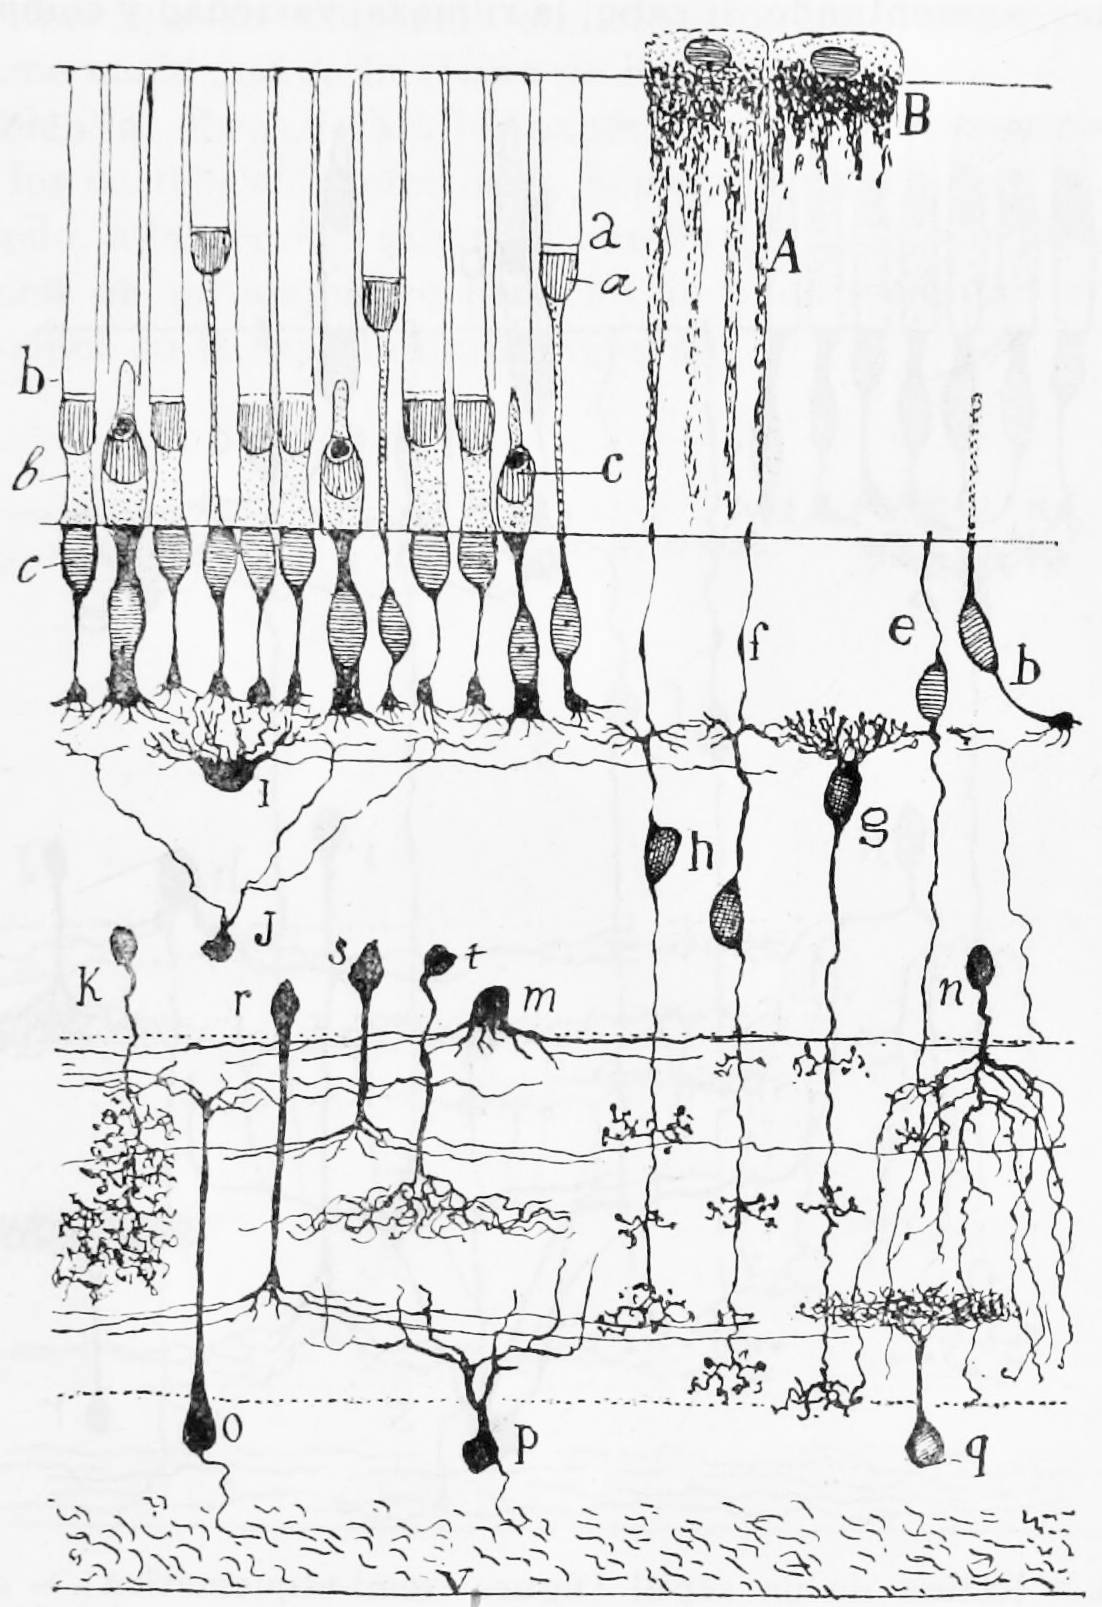
\includegraphics[width=0.7\linewidth]{./figures/sensation/FrogRetinaCajalManual} 

}

\caption{A semischematic diagram of the frog retina. a) green rods; b (left) red rods; c) cone; i) horizontal cell; h) bipolar cell; n,m,r,s,t) amacrine cells; o,p) ganglion cells; q) displaced amacrine cell. A) Pigment epithelial cell with extended process; B) Pigment epithelial cell with retracted process.}\label{fig:frogretina}
\end{figure}

The central retina predominantly contains cones, while the peripheral retina predominantly contains rods. At the centre of the macula is the foveal pit where the cones are narrow and long, and, arranged in a hexagonal mosaic, the most dense, in contradistinction to the much fatter cones located more peripherally in the retina. At the foveal pit the other retinal layers are displaced, before building up along the foveal slope until the rim of the fovea, or parafovea, is reached, which is the thickest portion of the retina. The macula has a yellow pigmentation and is known as the macula lutea. The area directly surrounding the fovea has the highest density of rods converging on single bipolar cells. Since its cones have a much lesser convergence of signals, the fovea allows for the sharpest vision the eye can attain.

Though the rod and cones are a mosaic of sorts, transmission from receptors, to bipolars, to ganglion cells is not direct. Since there are about 150 million receptors and only 1 million optic nerve fibres, there must be convergence and thus mixing of signals. Moreover, the horizontal action of the horizontal and amacrine cells can allow one area of the retina to control another (e.g.~one stimulus inhibiting another). This inhibition is key to lessening the sum of messages sent to the higher regions of the brain. In some lower vertebrates (e.g.~the pigeon), there is a ``centrifugal'' control of messages -- that is, one layer can control another, or higher regions of the brain can drive the retinal nerve cells, but in primates this does not occur.

\hypertarget{the-photoreceptors}{%
\subsection{The Photoreceptors}\label{the-photoreceptors}}

A photoreceptor cell is a specialized type of neuroepithelial cell found in the retina that is capable of visual phototransduction. The great biological importance of photoreceptors is that they convert light (visible electromagnetic radiation) into signals that can stimulate biological processes. To be more specific, photoreceptor proteins in the cell absorb photons, triggering a change in the cell's membrane potential.

There are currently three known types of photoreceptor cells in mammalian eyes: rods, cones, and intrinsically photosensitive retinal ganglion cells. The two classic photoreceptor cells are rods and cones, each contributing information used by the visual system to form a representation of the visual world, sight. The rods are narrower than the cones and distributed differently across the retina, but the chemical process in each that supports phototransduction is similar. A third class of mammalian photoreceptor cell was discovered during the 1990s: the intrinsically photosensitive retinal ganglion cells. These cells do not contribute to sight directly, but are thought to support circadian rhythms and pupillary reflex.



\begin{figure}

{\centering 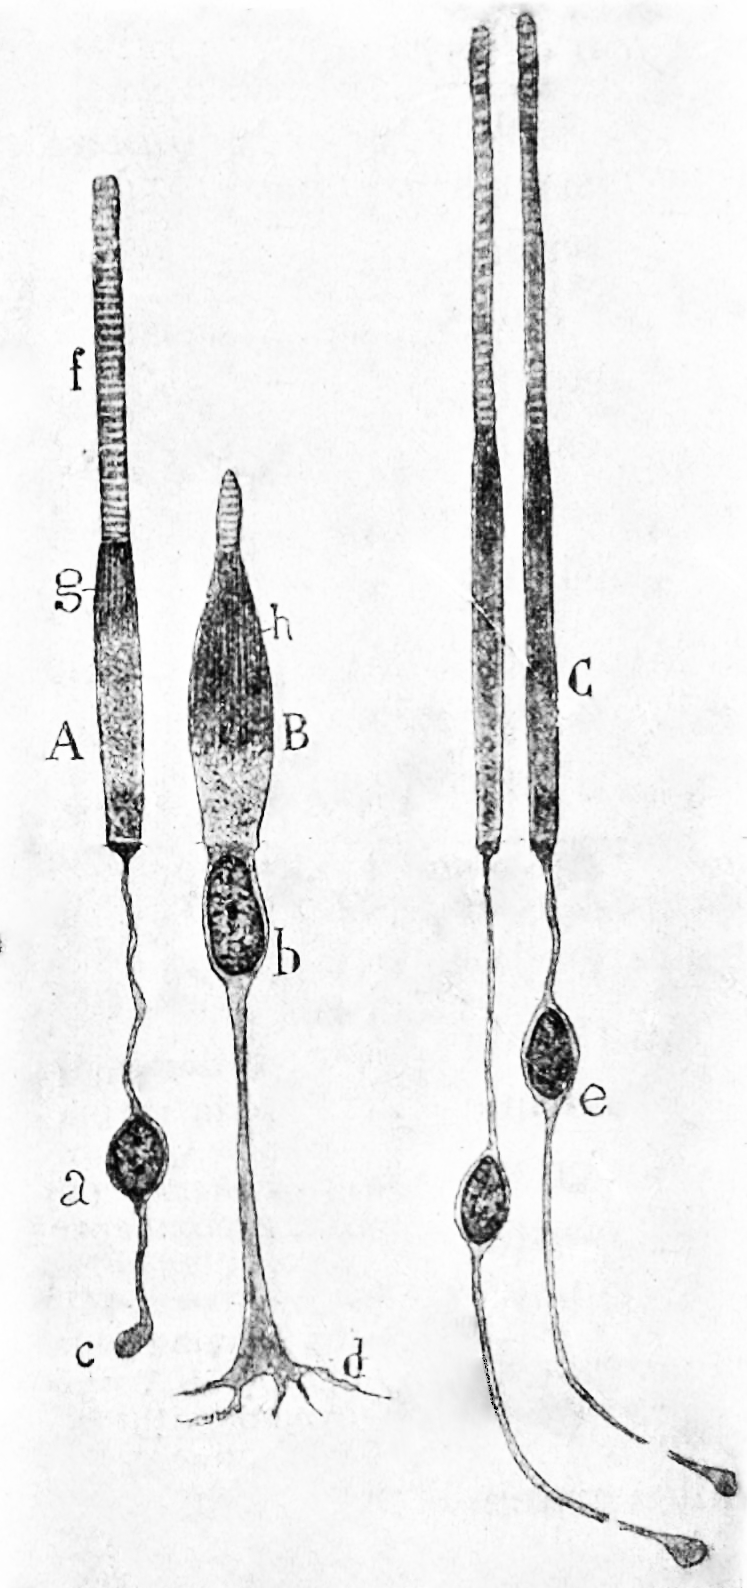
\includegraphics[width=0.7\linewidth]{./figures/sensation/PhotorecptorsCajalManual} 

}

\caption{Rods and cones from the human retina. A) a rod from the peripheral retina; B) a cone from the peripheral retina; C) cones from the fovea.}\label{fig:photoreceptors}
\end{figure}

There are major functional differences between the rods and cones. Rods are extremely sensitive, and can be triggered by a single photon. At very low light levels, visual experience is based solely on the rod signal.

Cones require significantly brighter light (that is, a larger number of photons) to produce a signal. In humans, there are three different types of cone cell, distinguished by their pattern of response to light of different wavelengths. Color experience is calculated from these three distinct signals. This explains why colors cannot be seen at low light levels, when only the rod and not the cone photoreceptor cells are active. The three types of cone cell respond (roughly) to light of short, medium, and long wavelengths, so they may respectively be referred to as S-cones, M-cones, and L-cones. The different responses of the three types of cone cells are determined by the likelihoods that their respective photoreceptor proteins will absorb photons of different wavelengths. So, for example, an L cone cell contains a photoreceptor protein that more readily absorbs long wavelengths of light (that is, more ``red''). Light of a shorter wavelength can also produce the same response, but it must be much brighter to do so.

The number and ratio of rods to cones varies among species, dependent on whether an animal is primarily diurnal or nocturnal.

\hypertarget{visual-phototransduction}{%
\subsection{Visual Phototransduction}\label{visual-phototransduction}}

Visual phototransduction is the sensory transduction of the visual system. It is a process by which light is converted into electrical signals in the rod cells, cone cells and photosensitive ganglion cells of the retina of the eye. This cycle was elucidated by \href{https://en.wikipedia.org/wiki/George_Wald}{George Wald} (1906--1997) for which he received the Nobel Prize in 1967.

The visual cycle is the biological conversion of a photon into an electrical signal in the retina. This process occurs via G-protein coupled receptors called opsins which contain the chromophore 11-cis retinal. 11-cis retinal is covalently linked to the opsin receptor via Schiff base forming retinylidene protein. When struck by a photon, 11-cis retinal undergoes photoisomerization to all-trans retinal which changes the conformation of the opsin GPCR leading to signal transduction cascades which causes closure of cyclic GMP-gated cation channel, and hyperpolarization of the photoreceptor cell.

Following isomerization and release from the opsin protein, all-trans retinal is reduced to all-trans retinol and travels back to the retinal pigment epithelium to be ``recharged''. It is first esterified by lecithin retinol acyltransferase (LRAT) and then converted to 11-cis retinol by the isomerohydrolase RPE65. Finally, it is oxidized to 11-cis retinal before traveling back to the rod outer segment where it is again conjugated to an opsin to form new, functional visual pigment (rhodopsin).

To understand the photoreceptor's behaviour to light intensities, it is necessary to understand the roles of different currents.



\begin{figure}

{\centering 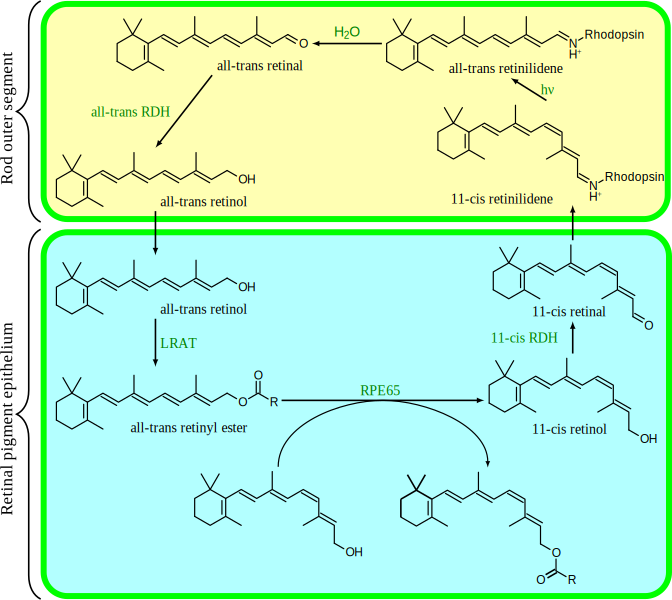
\includegraphics[width=0.7\linewidth]{./figures/sensation/Visual_cycle} 

}

\caption{\href{https://commons.wikimedia.org/wiki/File:Visual_cycle.svg}{The chemical reactions involved in the photoreceptor visual cycle.}}\label{fig:absorption}
\end{figure}

There is an ongoing outward potassium current through nongated K\textsuperscript{+}-selective channels. This outward current tends to hyperpolarize the photoreceptor at around -70 mV (the equilibrium potential for K\textsuperscript{+}).

There is also an inward sodium current carried by cGMP-gated sodium channels. This so-called `dark current' depolarizes the cell to around -40 mV. Note that this is significantly more depolarized than most other neurons.

A high density of Na\textsuperscript{+}-K\textsuperscript{+} pumps enables the photoreceptor to maintain a steady intracellular concentration of Na\textsuperscript{+} and K\textsuperscript{+}.

Photoreceptor cells are unusual cells in that they are depolarized under scotopic conditions (darkness). In photopic conditions (light), photoreceptors are hyperpolarized to a potential of -60mV.

In the dark, cGMP levels are high and keep cGMP-gated sodium channels open allowing a steady inward current, called the dark current. This dark current keeps the cell depolarized at about -40 mV, leading to glutamate release.

The depolarization of the cell membrane in scotopic conditions opens voltage-gated calcium channels. An increased intracellular concentration of Ca\textsuperscript{2+} causes vesicles containing glutamate, the photoreceptor neurotransmitter, to merge with the cell membrane, therefore releasing glutamate.

In the cone pathway glutamate

\begin{itemize}
\tightlist
\item
  Hyperpolarizes on-center bipolar cells. Glutamate that is released from the photoreceptors in the dark binds to metabotropic glutamate receptors (mGluR6), which, through a G-protein coupling mechanism, causes non-specific cation channels in the cells to close, thus hyperpolarizing the bipolar cell.
\item
  Depolarizes off-center bipolar cells. Binding of glutamate to ionotropic glutamate receptors results in an inward cation current that depolarizes the bipolar cell.
\end{itemize}

Activation of the phototransduction cascade

\begin{enumerate}
\def\labelenumi{\arabic{enumi}.}
\tightlist
\item
  A light photon interacts with the retinal in a photoreceptor cell. The retinal undergoes isomerisation, changing from the 11-cis to all-trans configuration.
\item
  Opsin therefore undergoes a conformational change to metarhodopsin II.
\item
  Metarhodopsin II activates a G protein known as transducin. This causes transducin to dissociate from its bound GDP, and bind GTP, then the alpha subunit of transducin dissociates from the beta and gamma subunits, with the GTP still bound to the alpha subunit.
\item
  The alpha subunit-GTP complex activates phosphodiesterase, also known as PDE6. It binds to one of two regulatory subunits of PDE (which itself is a tetramer) and inhibits its activity.
\item
  PDE hydrolyzes cGMP, forming GMP. This lowers the intracellular concentration of cGMP and therefore the sodium channels close.
\item
  Closure of the sodium channels causes hyperpolarization of the cell due to the ongoing efflux of potassium ions.
\item
  Hyperpolarization of the cell causes voltage-gated calcium channels to close.
\item
  As the calcium level in the photoreceptor cell drops, the amount of the neurotransmitter glutamate that is released by the cell also drops. This is because calcium is required for the glutamate-containing vesicles to fuse with cell membrane and release their contents (see SNARE proteins).
\item
  A decrease in the amount of glutamate released by the photoreceptors causes depolarization of on-center bipolar cells (rod and cone On bipolar cells) and hyperpolarization of cone off-center bipolar cells.
\end{enumerate}



\begin{figure}

{\centering 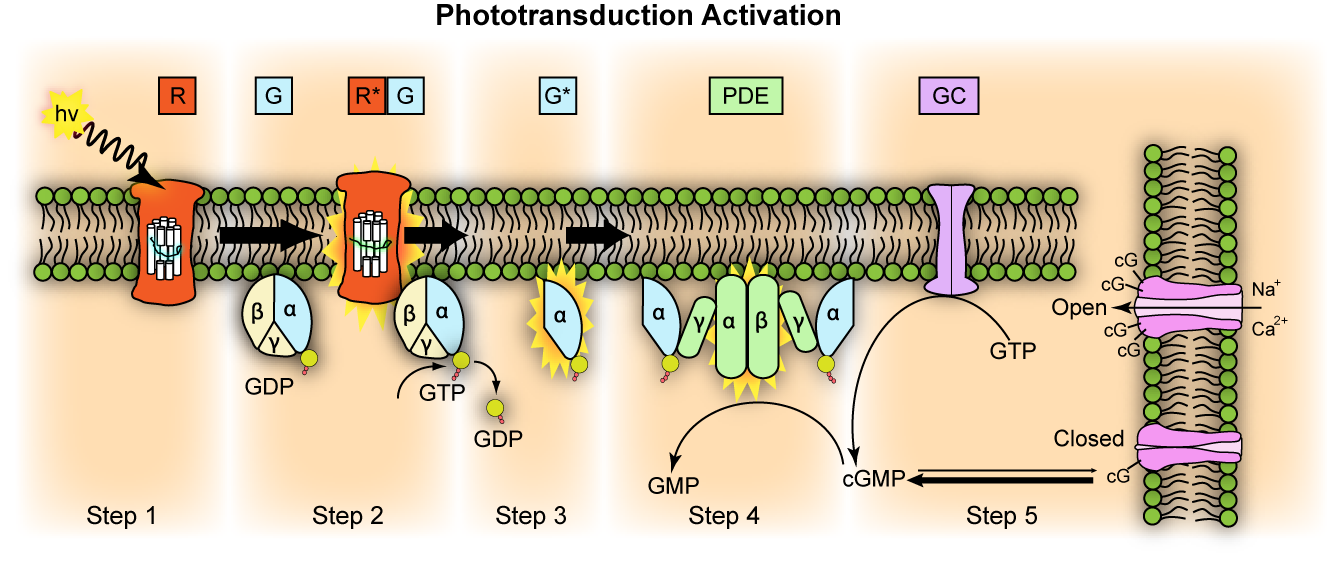
\includegraphics[width=0.7\linewidth]{./figures/sensation/Phototransduction} 

}

\caption{\href{https://commons.wikimedia.org/wiki/File:Phototransduction.png}{Representation} of molecular steps in photoactivation (modified from Leskov et al., 2000). Depicted is an outer membrane disk in a rod. Step 1: Incident photon (hν) is absorbed and activates a rhodopsin by conformational change in the disk membrane to R\emph{. Step 2: Next, R} makes repeated contacts with transducin molecules, catalyzing its activation to G* by the release of bound GDP in exchange for cytoplasmic GTP, which expels its β and γ subunits. Step 3: G* binds inhibitory γ subunits of the phosphodiesterase (PDE) activating its α and β subunits. Step 4: Activated PDE hydrolyzes cGMP. Step 5: Guanylyl cyclase (GC) synthesizes cGMP, the second messenger in the phototransduction cascade. Reduced levels of cytosolic cGMP cause cyclic nucleotide gated channels to close preventing further influx of Na\textsuperscript{+} and Ca\textsuperscript{2+}.}\label{fig:molsteps}
\end{figure}

Deactivation of the phototransduction cascade

In light, low cGMP levels close Na\textsuperscript{+} and Ca\textsuperscript{2+} channels, reducing intracellular Na\textsuperscript{+} and Ca\textsuperscript{2+}. During recovery (dark adaptation), the low Ca\textsuperscript{2+} levels induce recovery (termination of the phototransduction cascade), as follows:

\begin{enumerate}
\def\labelenumi{\arabic{enumi}.}
\tightlist
\item
  Low intracellular Ca\textsuperscript{2+} makes intracellular Ca-GCAP (Ca-Guanylate cyclase activating protein) dissociate into Ca\textsuperscript{2+} and GCAP. The liberated GCAP ultimately restores depleted cGMP levels, which re-opens the cGMP-gated cation channels (restoring dark current).
\item
  Low intracellular Ca\textsuperscript{2+} makes intracellular Ca-GAP (Ca-GTPase Accelerating Protein) dissociate into Ca\textsuperscript{2+} and GAP. The liberated GAP deactivates activated-transducin, terminating the phototransduction cascade (restoring dark current).
\item
  Low intracellular Ca\textsuperscript{2+} makes intracellular Ca-recoverin-RK dissociate into Ca\textsuperscript{2+} and recoverin and RK. The liberated RK then phosphorylates metarhodopsin II, reducing its binding affinity for transducin. Arrestin then completely deactivates the phosphorylated-metarhodopsin II, terminating the phototransduction cascade (restoring dark current).
\item
  Low intracellular Ca\textsuperscript{2+} make the Ca\textsuperscript{2+}/calmodulin complex within the cGMP-gated cation channels more sensitive to low cGMP levels (thereby, keeping the cGMP-gated cation channel open even at low cGMP levels, restoring dark current)
\end{enumerate}

All-trans retinal cannot be synthesised by humans and must be supplied by vitamin A in the diet. Deficiency of all-trans retinal can lead to night blindness. This is part of the bleach and recycle process of retinoids in the photoreceptors and retinal pigment epithelium.

Photoreceptor cells are typically arranged in an irregular but approximately hexagonal grid, known as the retinal mosaic.

The opsin found in the intrinsically photosensitive ganglion cells of the retina is called melanopsin. These cells are involved in various reflexive responses of the brain and body to the presence of (day)light, such as the regulation of circadian rhythms, pupillary reflex and other non-visual responses to light. Melanopsin functionally resembles invertebrate opsins.

\hypertarget{the-visual-pathways}{%
\subsection{The Visual Pathways}\label{the-visual-pathways}}

\hypertarget{the-optic-nerve-and-optic-tract}{%
\subsection{The Optic Nerve And Optic Tract}\label{the-optic-nerve-and-optic-tract}}

The optic nerve conducts the action potentials generated by the retinal ganglion cells through the optic canal to the subsequent processing centers in the brain. Upon reaching the optic chiasm the nerve fibers from the nasal part of the retina in each eye cross over to the other side (decussate). The fibers then branch and terminate in three places.

\begin{figure}

{\centering 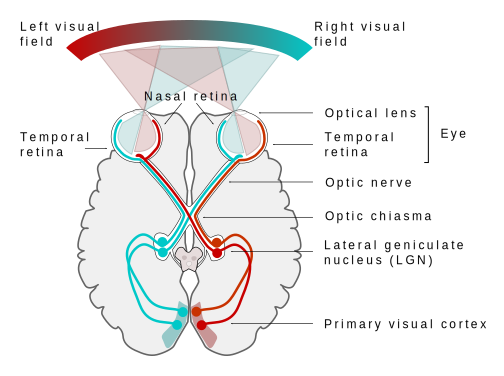
\includegraphics[width=0.7\linewidth]{./figures/sensation/Human_visual_pathway} 

}
\caption{\href{https://commons.m.wikimedia.org/wiki/File:human_visual_pathway.sv}{A simplified schema} of the human visual pathway.}\label{fig:visualpathways}
\end{figure}

The optic nerve is composed of retinal ganglion cell axons and glial cells. Each human optic nerve contains between 770,000 and 1.7 million nerve fibers, which are axons of the retinal ganglion cells of one retina.

In humans, the optic nerve is derived from optic stalks during the seventh week of development. It extends from the optic disc to the optic chiasma and continues as the optic tract to the lateral geniculate nucleus, pretectal nuclei, and superior colliculus.

Most of the axons of the optic nerve terminate in the lateral geniculate nucleus from where information is relayed to the visual cortex, while other axons terminate in the pretectal nucleus and are involved in reflexive eye movements. Other axons terminate in the suprachiasmatic nucleus and are involved in regulating the sleep-wake cycle. Its diameter increases from about 1.6 mm within the eye to 3.5 mm in the orbit to 4.5 mm within the cranial space.

\hypertarget{the-superior-colliculus}{%
\subsection{The Superior Colliculus}\label{the-superior-colliculus}}

The superior colliculus (Latin, upper hill) is a structure lying on the roof of the mammalian midbrain. In non-mammalian vertebrates the homologous structure, is known as the optic tectum or optic lobe.

In mammals the superior colliculus forms a major component of the midbrain. It is a paired structure and together with the paired inferior colliculi form the corpora quadrigemina (from Latin quadruplet bodies). The superior colliculus is a layered structure, with a number of layers that varies by species. The layers can be grouped into the superficial layers (stratum opticum and above) and the deeper remaining layers. Neurons in the superficial layers receive direct input from the retina and respond almost exclusively to visual stimuli. Many neurons in the deeper layers also respond to other modalities, and some respond to stimuli in multiple modalities. The deeper layers also contain a population of motor-related neurons, capable of activating eye movements as well as other responses.

The general function of the tectal system is to direct behavioral responses toward specific points in egocentric (``body-centered'') space. Each layer contains a topographic map of the surrounding world in retinotopic coordinates, and activation of neurons at a particular point in the map evokes a response directed toward the corresponding point in space. In primates, the superior colliculus has been studied mainly with respect to its role in directing eye movements. Visual input from the retina, or ``command'' input from the cerebral cortex, create a ``bump'' of activity in the tectal map, which, if strong enough, induces a saccadic eye movement. Even in primates, however, the superior colliculus is also involved in generating spatially directed head turns, arm-reaching movements, and shifts in attention that do not involve any overt movements. In mammals, and especially primates, the massive expansion of the cerebral cortex reduces the superior colliculus to a much smaller fraction of the whole brain. It remains nonetheless important in terms of function as the primary integrating center for eye movements.

Behavioral studies have shown that the SC is not needed for object recognition, but plays a critical role in the ability to direct behaviors toward specific objects, and can support this ability even in the absence of the cerebral cortex. Thus, cats with major damage to the visual cortex cannot recognize objects, but may still be able to follow and orient toward moving stimuli, although more slowly than usual. If one half of the SC is removed, however, the cats will circle constantly toward the side of the lesion, and orient compulsively toward objects located there, but fail to orient at all toward objects located in the opposite hemifield. These deficits diminish over time but never disappear.

In primates, eye movements can be divided into several types: fixation, in which the eyes are directed toward a motionless object, with eye movements only to compensate for movements of the head; smooth pursuit, in which the eyes move steadily to track a moving object; saccades, in which the eyes move very rapidly from one location to another; and vergence, in which the eyes move simultaneously in opposite directions to obtain or maintain single binocular vision. The superior colliculus is involved in all of these, but its role in saccades has been studied most intensively.

The output from the motor sector of the SC goes to a set of midbrain and brainstem nuclei, which transform the ``place'' code used by the SC into the ``rate'' code used by oculomotor neurons. Eye movements are generated by six muscles, arranged in three orthogonally-aligned pairs. Thus, at the level of the final common path, eye movements are encoded in essentially a Cartesian coordinate system.

Although the SC receives a strong input directly from the retina, in primates it is largely under the control of the cerebral cortex, which contains several areas that are involved in determining eye movements. The frontal eye fields, a portion of the motor cortex, are involved in triggering intentional saccades, and an adjoining area, the supplementary eye fields, are involved in organizing groups of saccades into sequences. The parietal eye fields, farther back in the brain, are involved mainly in reflexive saccades, made in response to changes in the view.

The SC only receives visual inputs in its superficial layers, whereas the deeper layers of the colliculus receive also auditory and somatosensory inputs and are connected to many sensorimotor areas of the brain. The colliculus as a whole is thought to help orient the head and eyes toward something seen and heard.

The superior colliculus also receives auditory information from the inferior colliculus. This auditory information is integrated with the visual information already present to produce the ventriloquist effect.

\hypertarget{the-lateral-geniculate-nucleus-lgn}{%
\subsection{The Lateral Geniculate Nucleus (LGN)}\label{the-lateral-geniculate-nucleus-lgn}}

The lateral geniculate nucleus (LGN; also called the lateral geniculate body or lateral geniculate complex; named after its resemblance to a bent knee) is a relay center in the thalamus for the visual pathway. It receives a major sensory input from the retina. The LGN is the main central connection for the optic nerve to the occipital lobe, particularly the primary visual cortex. In humans, each LGN has six layers of neurons (grey matter) alternating with optic fibers (white matter).

The LGN is a small, ovoid, ventral projection at the termination of the optic tract on each side of the brain. The LGN and the medial geniculate nucleus which deals with auditory information are both thalamic nuclei and so are present in both hemispheres.

The LGN receives information directly from the ascending retinal ganglion cells via the optic tract and from the reticular activating system. Neurons of the LGN send their axons through the optic radiation, a direct pathway to the primary visual cortex. In addition, the LGN receives many strong feedback connections from the primary visual cortex. In humans as well as other mammals, the two strongest pathways linking the eye to the brain are those projecting to the dorsal part of the LGN in the thalamus, and to the superior colliculus.

In humans as well as in many other primates, the LGN has layers of magnocellular cells and parvocellular cells that are interleaved with layers of koniocellular cells. In humans the LGN is normally described as having six distinctive layers. The inner two layers, (1 and 2) are magnocellular layers, while the outer four layers, (3,4,5 and 6), are parvocellular layers. An additional set of neurons, known as the koniocellular layers, are found ventral to each of the magnocellular and parvocellular layers.

The magnocellular, parvocellular, and koniocellular layers of the LGN correspond with the similarly named types of retinal ganglion cells. Retinal P ganglion cells send axons to a parvocellular layer, M ganglion cells send axons to a magnocellular layer, and K ganglion cells send axons to a koniocellular layer.:269

Koniocellular cells are functionally and neurochemically distinct from M and P cells and provide a third channel to the visual cortex. They project their axons between the layers of the lateral geniculate nucleus where M and P cells project. Their role in visual perception is presently unclear; however, the koniocellular system has been linked with the integration of somatosensory system-proprioceptive information with visual perception, and it may also be involved in color perception.

The other major retino--cortical visual pathway is the tectopulvinar pathway, routing primarily through the superior colliculus and thalamic pulvinar nucleus onto posterior parietal cortex and visual area MT.

Ipsilateral and contralateral layers

Layer 1, 2

\begin{itemize}
\tightlist
\item
  Large cells, called magnocellular pathways
\item
  Input from M-ganglion cells
\item
  Very rapid conduction
\item
  Colour blind system
\end{itemize}

Layer 3--6

\begin{itemize}
\tightlist
\item
  Parvocellular
\item
  Input from P-ganglion cells
\item
  Colour vision
\item
  Moderate velocity.
\end{itemize}

Both the LGN in the right hemisphere and the LGN in the left hemisphere receive input from each eye. However, each LGN only receives information from one half of the visual field. This occurs due to axons of the ganglion cells from the inner halves of the retina (the nasal sides) decussating (crossing to the other side of the brain) through the optic chiasma (khiasma means ``cross-shaped''). The axons of the ganglion cells from the outer half of the retina (the temporal sides) remain on the same side of the brain. Therefore, the right hemisphere receives visual information from the left visual field, and the left hemisphere receives visual information from the right visual field. Within one LGN, the visual information is divided among the various layers as follows:

\begin{itemize}
\tightlist
\item
  the eye on the same side (the ipsilateral eye) sends information to layers 2, 3 and 5
\item
  the eye on the opposite side (the contralateral eye) sends information to layers 1, 4 and 6.
\end{itemize}

This description applies to the LGN of many primates, but not all.

The principal neurons in the LGN receive strong inputs from the retina. However, the retina only accounts for a small percentage of LGN input. As much as 95\% of input in the LGN comes from the visual cortex, superior colliculus, pretectum, thalamic reticular nuclei, and local LGN interneurons. Regions in the brainstem that are not involved in visual perception also project to the LGN, such as the mesencephalic reticular formation, dorsal raphe nucleus, periaqueductal grey matter, and the locus coeruleus. These non-retinal inputs can be excitatory, inhibitory, or modulatory.

Information leaving the LGN travels out on the optic radiations, which form part of the retrolenticular portion of the internal capsule.

The axons that leave the LGN go to V1 visual cortex. Both the magnocellular layers 1--2 and the parvocellular layers 3--6 send their axons to layer 4 in V1. Within layer 4 of V1, layer 4cβ receives parvocellular input, and layer 4cα receives magnocellular input. However, the koniocellular layers, intercalated between LGN layers 1--6 send their axons primarily to the cytochrome-oxidase rich blobs of layers 2 and 3 in V1. Axons from layer 6 of visual cortex send information back to the LGN.

Studies involving blindsight have suggested that projections from the LGN travel not only to the primary visual cortex but also to higher cortical areas V2 and V3. Patients with blindsight are phenomenally blind in certain areas of the visual field corresponding to a contralateral lesion in the primary visual cortex; however, these patients are able to perform certain motor tasks accurately in their blind field, such as grasping. This suggests that neurons travel from the LGN to both the primary visual cortex and higher cortex regions.

\hypertarget{the-visual-cortex}{%
\subsection{The Visual Cortex}\label{the-visual-cortex}}

The visual cortex of the brain is that part of the cerebral cortex which processes visual information. It is located in the occipital lobe.

The visual cortex is the largest system in the human brain and is responsible for processing the visual information. The region that receives information directly from the LGN is called the primary visual cortex, (also called V1 and striate cortex). The primary visual cortex is the most studied visual area in the brain. Visual information then flows through a cortical hierarchy. These areas include V2, V3, V4 and area V5/MT (the exact connectivity depends on the species of the animal).

As visual information passes forward through the visual hierarchy, the complexity of the neural representations increases. Whereas a V1 neuron may respond selectively to a line segment of a particular orientation in a particular retinotopic location, neurons in the lateral occipital complex respond selectively to complete object (e.g., a figure drawing), and neurons in visual association cortex may respond selectively to human faces, or to a particular object.

\begin{figure}

{\centering 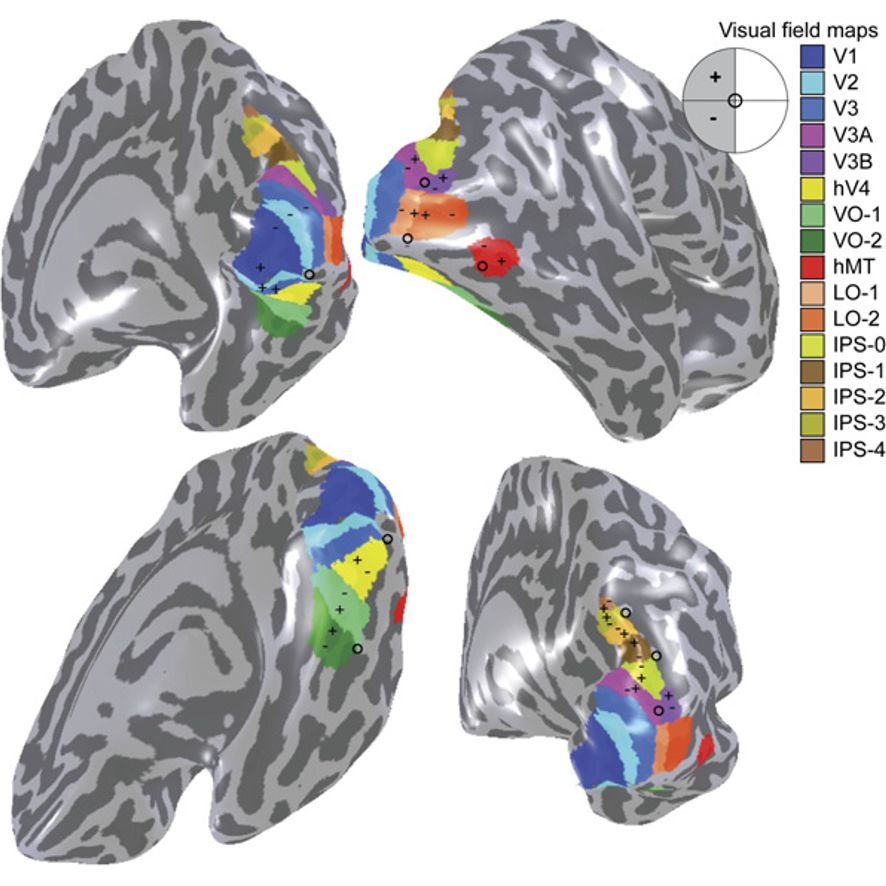
\includegraphics[width=0.7\linewidth]{./figures/sensation/Visual_field_maps} 
}
\caption{\href{https://commons.wikimedia.org/wiki/File:Visual_field_maps.jpg}{A
visual field map} of the primary visual cortex and the numerous
extrastriate areas.}\label{fig:visualcortex}
\end{figure}

Along with this increasing complexity of neural representation may come a level of specialization of processing into two distinct pathways: the dorsal stream and the ventral stream (the Two Streams hypothesis, first proposed by Ungerleider and Mishkin in 1982). The dorsal stream, commonly referred to as the ``where'' stream, is involved in spatial attention (covert and overt), and communicates with regions that control eye movements and hand movements. More recently, this area has been called the ``how'' stream to emphasize its role in guiding behaviors to spatial locations. The ventral stream, commonly referred as the ``what'' stream, is involved in the recognition, identification and categorization of visual stimuli.

However, there is still much debate about the degree of specialization within these two pathways, since they are in fact heavily interconnected.

Visual information coming from the eye goes through the lateral geniculate nucleus in the thalamus and then reaches the visual cortex. The part of the visual cortex that receives the sensory inputs from the thalamus is the primary visual cortex, also known as visual area 1 (V1, Brodmann area 17), and the striate cortex. The extrastriate areas consist of visual areas 2 (V2, Brodmann area 18), 3, 4, and 5 (V3, V4, V5, all Brodmann area 19).

The primary visual cortex (V1) is located in and around the calcarine fissure in the occipital lobe. Each hemisphere's V1 receives information directly from its ipsilateral lateral geniculate nucleus that receives signals from the contralateral visual hemifield.

Neurons in the visual cortex fire action potentials when visual stimuli appear within their receptive field. By definition, the receptive field is the region within the entire visual field that elicits an action potential. But, for any given neuron, it may respond best to a subset of stimuli within its receptive field. This property is called neuronal tuning. In the earlier visual areas, neurons have simpler tuning. For example, a neuron in V1 may fire to any vertical stimulus in its receptive field. In the higher visual areas, neurons have complex tuning. For example, in the inferior temporal cortex (IT), a neuron may fire only when a certain face appears in its receptive field.

The visual cortex receives its blood supply primarily from the calcarine branch of the posterior cerebral artery.

V1 transmits information to two primary pathways, called the ventral stream and the dorsal stream. The ventral stream begins with V1, goes through visual area V2, then through visual area V4, and to the inferior temporal cortex (IT cortex). The ventral stream, sometimes called the ``What Pathway'', is associated with form recognition and object representation. It is also associated with storage of long-term memory.
The dorsal stream begins with V1, goes through Visual area V2, then to the dorsomedial area (DM/V6) and medial temporal area (MT/V5) and to the posterior parietal cortex. The dorsal stream, sometimes called the ``Where Pathway'' or ``How Pathway'', is associated with motion, representation of object locations, and control of the eyes and arms, especially when visual information is used to guide saccades or reaching.

\hypertarget{the-auditory-and-vestibular-systems}{%
\section{The Auditory And Vestibular Systems}\label{the-auditory-and-vestibular-systems}}

The auditory system is the sensory system for the sense of hearing. It includes both the sensory organs (the ears) and the auditory parts of the sensory system. Hearing, or auditory perception, is the ability to perceive sounds by detecting vibrations, changes in the pressure of the surrounding medium over time, through the ear.

Providing balance, when moving or stationary, is also a central function of the ear. The ear facilitates two types of balance: static balance, which allows a person to feel the effects of gravity, and dynamic balance, which allows a person to sense acceleration.

\hypertarget{the-ear}{%
\subsection{The Ear}\label{the-ear}}

In mammals, the ear is usually described as having three parts---the outer ear, the middle ear and the inner ear. The outer ear consists of the pinna and the ear canal. The folds of cartilage surrounding the ear canal are called the pinna. Sound waves are reflected and attenuated when they hit the pinna, and these changes provide additional information that will help the brain determine the sound direction. Since the outer ear is the only visible portion of the ear in most animals, the word ``ear'' often refers to the external part alone. The middle ear includes the tympanic cavity and the three ossicles. The inner ear sits in the bony labyrinth, and contains structures which are key to several senses: the semicircular canals, which enable balance and eye tracking when moving; the utricle and saccule, which enable balance when stationary; and the cochlea, which enables hearing. The ears of vertebrates are placed somewhat symmetrically on either side of the head, an arrangement that aids sound localisation.

The ear develops from the first pharyngeal pouch and six small swellings that develop in the early embryo called otic placodes, which are derived from ectoderm.

The ear canal of the outer ear is separated from the air-filled tympanic cavity of the middle ear by the eardrum. The middle ear contains the three small bones---the ossicles---involved in the transmission of sound, and is connected to the throat at the nasopharynx, via the pharyngeal opening of the Eustachian tube. The inner ear contains the otolith organs---the utricle and saccule---and the semicircular canals belonging to the vestibular system, as well as the cochlea of the auditory system.



\begin{figure}

{\centering 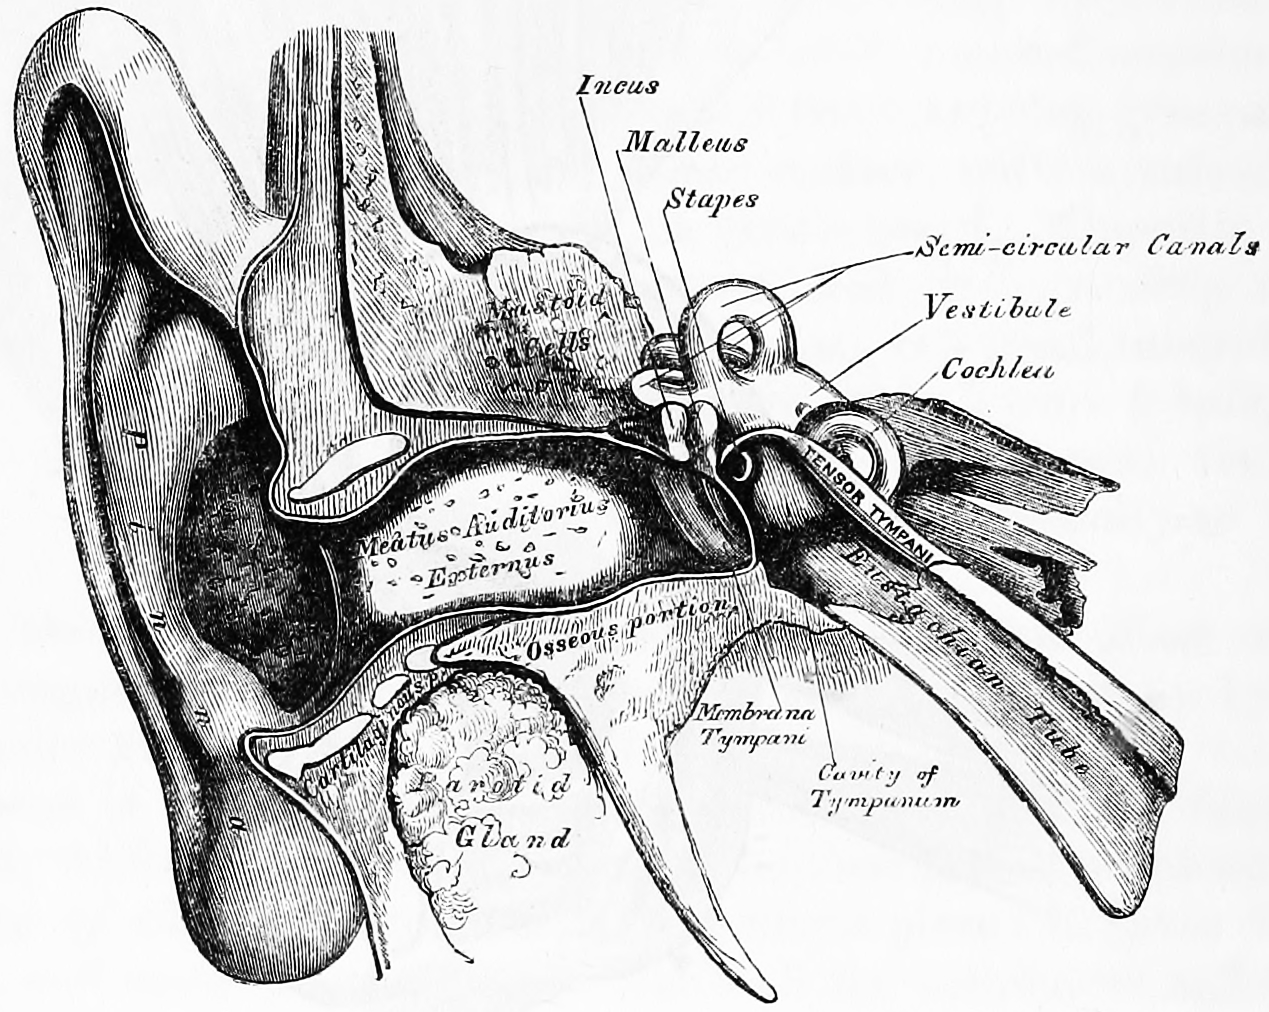
\includegraphics[width=0.7\linewidth]{./figures/sensation/GrayEar} 

}

\caption{Front view of the right outer, middle and inner human ear. \href{https://archive.org/details/anatomydescripti00grayuoft/page/n6/mode/2up}{Gray, Henry, 1825-1861. Anatomy, descriptive and surgical; ed.~by T. Pickering Pick and Robert Howden. A revised American, from the fifteenth English edition. Philadelphia, Lea, 1901}}\label{fig:rightear}
\end{figure}

Sound waves travel through the ear canal and hit the tympanic membrane, or eardrum. This wave information travels across the air-filled middle ear cavity via a series of delicate bones: the malleus (hammer), incus (anvil) and stapes (stirrup). These ossicles act as a lever, converting the lower-pressure eardrum sound vibrations into higher-pressure sound vibrations at another, smaller membrane called the oval window or vestibular window. The manubrium (handle) of the malleus articulates with the tympanic membrane, while the footplate (base) of the stapes articulates with the oval window. Higher pressure is necessary at the oval window than at the typanic membrane because the inner ear beyond the oval window contains liquid rather than air. The stapedius reflex of the middle ear muscles helps protect the inner ear from damage by reducing the transmission of sound energy when the stapedius muscle is activated in response to sound. The middle ear still contains the sound information in wave form; it is converted to nerve impulses in the cochlea.
The middle-ear ossicles further amplify the vibration pressure roughly 20 times. The base of the stapes couples vibrations into the cochlea via the oval window, which vibrates the perilymph liquid (present throughout the inner ear) and causes the round window to bulb out as the oval window bulges in.

The inner ear consists of the cochlea and several non-auditory structures. The cochlea has three fluid-filled sections (i.e.~the scala media, scala tympani and scala vestibuli), and supports a fluid wave driven by pressure across the basilar membrane separating two of the sections. Strikingly, one section, called the cochlear duct or scala media, contains endolymph. Endolymph is a fluid similar in composition to the intracellular fluid found inside cells. The organ of Corti is located in this duct on the basilar membrane, and transforms mechanical waves to electric signals in neurons. The other two sections are known as the scala tympani and the scala vestibuli. These are located within the bony labyrinth, which is filled with fluid called perilymph, similar in composition to cerebrospinal fluid. The chemical difference between the fluids endolymph and perilymph fluids is important for the function of the inner ear.

\hypertarget{the-auditory-system}{%
\section{The Auditory System}\label{the-auditory-system}}

In humans and other vertebrates, hearing is performed primarily by the auditory system: mechanical waves, known as vibrations, are detected by the ear and transduced into nerve impulses that are perceived by the brain (primarily in the temporal lobe). Like touch, audition requires sensitivity to the movement of molecules in the world outside the organism. Both hearing and touch are types of mechanosensation. Sound may be heard through solid, liquid, or gaseous matter. It is one of the traditional five senses; partial or total inability to hear is called hearing loss.

\hypertarget{organ-of-corti}{%
\subsection{Organ Of Corti}\label{organ-of-corti}}

The organ of Corti, or spiral organ, is the receptor organ for hearing and is located in the mammalian cochlea. This highly varied strip of epithelial cells allows for transduction of auditory signals into nerve impulses. Transduction occurs through vibrations of structures in the inner ear causing displacement of cochlear fluid and movement of hair cells at the organ of Corti to produce electrochemical signals.

Italian anatomist \href{https://en.wikipedia.org/wiki/Alfonso_Giacomo_Gaspare_Corti}{Alfonso Giacomo Gaspare Corti} (1822--1876) discovered the organ of corti in 1851.

The organ of corti is located in the scala media of the cochlea of the inner ear between the vestibular duct and the tympanic duct and is composed of mechanosensory cells, known as hair cells. strategically positioned on the basilar membrane of the organ of corti are three rows of outer hair cells (ohcs) and one row of inner hair cells (ihcs). Separating these hair cells are supporting cells: Deiters cells, also called phalangeal cells, which separate and support both the ohcs and the ihcs.



\begin{figure}

{\centering 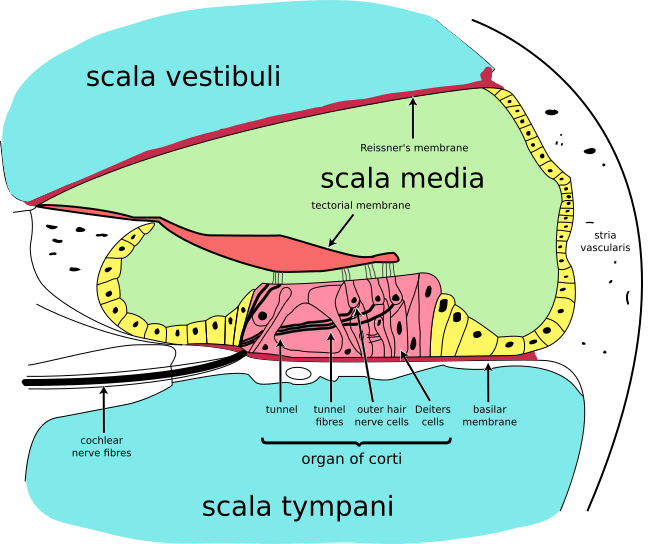
\includegraphics[width=0.7\linewidth]{./figures/sensation/Cochlea-crosssection} 

}

\caption{\href{https://commons.wikimedia.org/wiki/File:Cochlea-crosssection.svg}{A cross section of the cochlea illustrating the organ of Corti.}}\label{fig:organcorti}
\end{figure}

Projecting from the tips of the hair cells are tiny finger like projections called stereocilia, which are arranged in a graduated fashion with the shortest stereocilia on the outer rows and the longest in the center.

If the cochlea were uncoiled it would roll out to be about 33 mm long in women and 34 mm in men, with about 2.28 mm of standard deviation for the population. The cochlea is also tonotopically organized, meaning that different frequencies of sound waves interact with different locations on the structure. The base of the cochlea, closest to the outer ear, is the most stiff and narrow and is where the high frequency sounds are transduced. The apex, or top, of the cochlea is wider and much more flexible and loose and functions as the transduction site for low frequency sounds.

\hypertarget{auditory-transduction}{%
\subsection{Auditory Transduction}\label{auditory-transduction}}

In normal hearing subjects, the majority of the auditory signals that reach the organ of Corti in the first place come from the outer ear. Sound waves enter through the auditory canal and vibrate the tympanic membrane, also known as the eardrum, which vibrates three small bones called the ossicles. As a result, the attached oval window moves and causes movement of the round window, which leads to displacement of the cochlear fluid. However, the stimulation can happen also via direct vibration of the cochlea from the skull. The latter is referred to as Bone Conduction (or BC) hearing, as complementary to the first one described, which is instead called Air Conduction (or AC) hearing. Both AC and BC stimulate the basilar membrane in the same way.

The basilar membrane on the tympanic duct presses against the hair cells of the organ as perilymphatic pressure waves pass. The stereocilia atop the IHCs move with this fluid displacement and in response their cation, or positive ion selective, channels are pulled open by cadherin structures called tip links that connect adjacent stereocilia. The organ of Corti, surrounded in potassium rich fluid endolymph, lies on the basilar membrane at the base of the scala media. Under the organ of Corti is the scala tympani and above it, the scala vestibuli. Both structures exist in a low potassium fluid called perilymph. Because those stereocilia are in the midst of a high concentration of potassium, once their cation channels are pulled open, potassium ions as well as calcium ions flow into the top of the hair cell. With this influx of positive ions the IHC becomes depolarized, opening voltage-gated calcium channels at the basolateral region of the hair cells and triggering the release of the neurotransmitter glutamate. An electrical signal is then sent through the auditory nerve and into the auditory cortex of the brain as a neural message.

The organ of Corti is also capable of modulating the auditory signal. The outer hair cells (OHCs) can amplify the signal through a process called electromotility where they increase movement of the basilar and tectorial membranes and therefore increase deflection of stereocilia in the IHCs.

A crucial piece to this cochlear amplification is the motor protein prestin, which changes shape based on the voltage potential inside of the hair cell. When the cell is depolarized, prestin shortens, and because it is located on the membrane of OHCs it then pulls on the basilar membrane and increasing how much the membrane is deflected, creating a more intense effect on the inner hair cells (IHCs). When the cell hyperpolarizes prestin lengthens and eases tension on the IHCs, which decreases the neural impulses to the brain. In this way, the hair cell itself is able to modify the auditory signal before it even reaches the brain.

Hair cells are columnar cells, each with a bundle of 100--200 specialized cilia at the top, for which they are named. There are two types of hair cells; inner and outer hair cells. Inner hair cells are the mechanoreceptors for hearing: they transduce the vibration of sound into electrical activity in nerve fibers, which is transmitted to the brain. Outer hair cells are a motor structure. Sound energy causes changes in the shape of these cells, which serves to amplify sound vibrations in a frequency specific manner. Lightly resting atop the longest cilia of the inner hair cells is the tectorial membrane, which moves back and forth with each cycle of sound, tilting the cilia, which is what elicits the hair cells' electrical responses.

Inner hair cells, like the photoreceptor cells of the eye, show a graded response, instead of the spikes typical of other neurons.

\hypertarget{auditory-pathways}{%
\subsection{Auditory Pathways}\label{auditory-pathways}}

Afferent neurons innervate cochlear inner hair cells, at synapses where the neurotransmitter glutamate communicates signals from the hair cells to the dendrites of the primary auditory neurons.

There are far fewer inner hair cells in the cochlea than afferent nerve fibers -- many auditory nerve fibers innervate each hair cell. The neural dendrites belong to neurons of the auditory nerve, which in turn joins the vestibular nerve to form the vestibulocochlear nerve, or cranial nerve number VIII. The region of the basilar membrane supplying the inputs to a particular afferent nerve fibre can be considered to be its receptive field.

Efferent projections from the brain to the cochlea also play a role in the perception of sound, although this is not well understood. Efferent synapses occur on outer hair cells and on afferent (towards the brain) dendrites under inner hair cells

\hypertarget{the-cochlear-nucleus}{%
\subsection{The Cochlear Nucleus}\label{the-cochlear-nucleus}}

The cochlear nucleus is the first site of the neuronal processing of the newly converted ``digital'' data from the inner ear. In mammals, this region is anatomically and physiologically split into two regions, the dorsal cochlear nucleus (DCN), and ventral cochlear nucleus (VCN).

\hypertarget{the-trapezoid-body}{%
\subsection{The Trapezoid Body}\label{the-trapezoid-body}}

The trapezoid body is a bundle of decussating fibers in the ventral pons that carry information used for binaural computations in the brainstem. Some of these axons come from the cochlear nucleus and cross over to the other side before traveling on to the superior olivary nucleus. This is believed to help with localization of sound.

\hypertarget{the-superior-olivary-complex}{%
\subsection{The superior olivary complex}\label{the-superior-olivary-complex}}

The superior olivary complex is located in the pons, and receives projections predominantly from the ventral cochlear nucleus, although the dorsal cochlear nucleus projects there as well, via the ventral acoustic stria. Within the superior olivary complex lies the lateral superior olive (LSO) and the medial superior olive (MSO). The former is important in detecting interaural level differences while the latter is important in distinguishing interaural time difference.

\hypertarget{the-lateral-lemniscus}{%
\subsection{The Lateral Lemniscus}\label{the-lateral-lemniscus}}

The lateral lemniscus is a tract of axons in the brainstem that carries information about sound from the cochlear nucleus to various brainstem nuclei and ultimately the contralateral inferior colliculus of the midbrain.

\hypertarget{the-inferior-colliculi}{%
\subsection{The Inferior Colliculi}\label{the-inferior-colliculi}}

The inferior colliculi (IC) are located just below the visual processing centers known as the superior colliculi. The central nucleus of the IC is a nearly obligatory relay in the ascending auditory system, and most likely acts to integrate information (specifically regarding sound source localization from the superior olivary complex and dorsal cochlear nucleus) before sending it to the thalamus and cortex.

\hypertarget{the-medial-geniculate-nucleus-mgn}{%
\subsection{The Medial Geniculate Nucleus (MGN)}\label{the-medial-geniculate-nucleus-mgn}}

The medial geniculate nucleus is part of the thalamic relay system.

\hypertarget{the-primary-auditory-cortex}{%
\subsection{The Primary Auditory Cortex}\label{the-primary-auditory-cortex}}

The primary auditory cortex is the first region of cerebral cortex to receive auditory input.

Perception of sound is associated with the left posterior superior temporal gyrus (STG). The superior temporal gyrus contains several important structures of the brain, including Brodmann areas 41 and 42, marking the location of the primary auditory cortex, the cortical region responsible for the sensation of basic characteristics of sound such as pitch and rhythm. We know from research in nonhuman primates that the primary auditory cortex can probably be divided further into functionally differentiable subregions. The neurons of the primary auditory cortex can be considered to have receptive fields covering a range of auditory frequencies and have selective responses to harmonic pitches. Neurons integrating information from the two ears have receptive fields covering a particular region of auditory space.

The primary auditory cortex is surrounded by secondary auditory cortex, and interconnects with it. These secondary areas interconnect with further processing areas in the superior temporal gyrus, in the dorsal bank of the superior temporal sulcus, and in the frontal lobe. In humans, connections of these regions with the middle temporal gyrus are probably important for speech perception. The frontotemporal system underlying auditory perception allows us to distinguish sounds as speech, music, or noise.

\hypertarget{the-auditory-ventral-and-dorsal-streams}{%
\subsection{The Auditory Ventral And Dorsal Streams}\label{the-auditory-ventral-and-dorsal-streams}}

From the primary auditory cortex emerge two separate pathways: the auditory ventral stream and auditory dorsal stream. The auditory ventral stream includes the anterior superior temporal gyrus, anterior superior temporal sulcus, middle temporal gyrus and temporal pole. Neurons in these areas are responsible for sound recognition, and extraction of meaning from sentences. The auditory dorsal stream includes the posterior superior temporal gyrus and sulcus, inferior parietal lobule and intra-parietal sulcus. Both pathways project in humans to the inferior frontal gyrus. The most established role of the auditory dorsal stream in primates is sound localization. In humans, the auditory dorsal stream in the left hemisphere is also responsible for speech repetition and articulation, phonological long-term encoding of word names, and verbal working memory.

\hypertarget{the-vestibular-system}{%
\section{The Vestibular System}\label{the-vestibular-system}}

The vestibular system, in vertebrates, is part of the inner ear. In most mammals, the vestibular system is the sensory system that provides the leading contribution to the sense of balance and spatial orientation for the purpose of coordinating movement with balance. Together with the cochlea, a part of the auditory system, it constitutes the labyrinth of the inner ear in most mammals. As movements consist of rotations and translations, the vestibular system comprises two components: the semicircular canals which indicate rotational movements; and the otoliths which indicate linear accelerations. The vestibular system sends signals primarily to the neural structures that control eye movements, and to the muscles that keep an animal upright and in general control posture. The projections to the former provide the anatomical basis of the vestibulo-ocular reflex, which is required for vision; while the projections to the latter provide the anatomical means required to enable an animal to maintain its position in space.

The brain uses information from the vestibular system in the head and from proprioception throughout the body to enable the animal to understand its body's dynamics and kinematics (including its position and acceleration) from moment to moment. How these two perceptive sources are integrated to provide the underlying structure of the sensorium is unknown.

\hypertarget{the-semicircular-canals}{%
\subsection{The Semicircular Canals}\label{the-semicircular-canals}}

The semicircular canal system detects rotational movements.

The semicircular canals are a component of the bony labyrinth that are at right angles to each other. At one end of each of the semicircular canals is a dilated sac called an osseous ampulla which is more than twice the diameter of the canal. Each ampulla contains an ampulla crest, the crista ampullaris which consists of a thick gelatinous cap called a cupula and many hair cells. The superior and posterior semicircular canals are oriented vertically at right angles to each other. The lateral semicircular canal is about a 30-degree angle from the horizontal plane. The orientations of the canals cause a different canal to be stimulated by movement of the head in different planes, and more than one canal is stimulated at once if the movement is off those planes. The horizontal canal detects angular acceleration of the head when the head is turned and the superior and posterior canals detect vertical head movements when the head is moved up or down. When the head changes position, the endolymph in the canals lags behind due to inertia and this acts on the cupula which bends the cilia of the hair cells. The stimulation of the hair cells sends the message to the brain that acceleration is taking place. The ampullae open into the vestibule by five orifices, one of the apertures being common to two of the canals.

Since the world is three-dimensional, the vestibular system contains three semicircular canals in each labyrinth. They are approximately orthogonal (at right angles) to each other, and are the horizontal (or lateral), the anterior semicircular canal (or superior), and the posterior (or inferior) semicircular canal. Anterior and posterior canals may collectively be called vertical semicircular canals.

The anterior and posterior semicircular canals detect rotations of the head in the sagittal plane (as when nodding), and in the frontal plane, as when cartwheeling. Both anterior and posterior canals are orientated at approximately 45° between frontal and sagittal planes.
The movement of fluid pushes on a structure called the cupula which contains hair cells that transduce the mechanical movement to electrical signals.

The canals are arranged in such a way that each canal on the left side has an almost parallel counterpart on the right side. Each of these three pairs works in a push-pull fashion: when one canal is stimulated, its corresponding partner on the other side is inhibited, and vice versa.

\hypertarget{the-otolithic-organs}{%
\subsection{The Otolithic Organs}\label{the-otolithic-organs}}

While the semicircular canals respond to rotations, the otolithic organs sense linear accelerations. Humans have two otolithic organs on each side, one called the utricle, the other called the saccule. The utricle contains a patch of hair cells and supporting cells called a macula. Similarly, the saccule contains a patch of hair cells and a macula. Each hair cell of a macula has 40-70 stereocilia and one true cilium called a kinocilium. The tips of these cilia are embedded in an otolithic membrane. This membrane is weighted down with protein-calcium carbonate granules called otoconia. These otoconia add to the weight and inertia of the membrane and enhance the sense of gravity and motion. With the head erect, the otolithic membrane bears directly down on the hair cells and stimulation is minimal. When the head is tilted, however, the otolithic membrane sags and bends the stereocilia, stimulating the hair cells. Any orientation of the head causes a combination of stimulation to the utricles and saccules of the two ears. The brain interprets head orientation by comparing these inputs to each other and to other input from the eyes and stretch receptors in the neck, thereby detecting whether the head is tilted or the entire body is tipping. Essentially, these otolithic organs sense how quickly you are accelerating forward or backward, left or right, or up or down. Most of the utricular signals elicit eye movements, while the majority of the saccular signals projects to muscles that control our posture.

While the interpretation of the rotation signals from the semicircular canals is straightforward, the interpretation of otolith signals is more difficult: since gravity is equivalent to a constant linear acceleration, one somehow has to distinguish otolith signals that are caused by linear movements from those caused by gravity. Humans can do that quite well, but the neural mechanisms underlying this separation are not yet fully understood. Humans can sense head tilting and linear acceleration even in dark environments because of the orientation of two groups of hair cell bundles on either side of the striola. Hair cells on opposite sides move with mirror symmetry, so when one side is moved, the other is inhibited. The opposing effects caused by a tilt of the head cause differential sensory inputs from the hair cell bundles allow humans to tell which way the head is tilting, Sensory information is then sent to the brain, which can respond with appropriate corrective actions to the nervous and muscular systems to ensure that balance and awareness are maintained.

Diseases of the vestibular system can take different forms, and usually induce vertigo and instability or loss of balance, often accompanied by nausea.

When the vestibular system and the visual system deliver incongruous results, nausea often occurs. When the vestibular system reports no movement but the visual system reports movement, the motion disorientation is often called motion sickness (or seasickness, car sickness, simulation sickness, or airsickness). In the opposite case, such as when a person is in a zero-gravity environment or during a virtual reality session, the disoriented sensation is often called space sickness or space adaptation syndrome. Either of these ``sicknesses'' usually ceases once the congruity between the two systems is restored.

Each canal is filled with a fluid called endolymph and contains motion sensors within the fluids. At the base of each canal, the bony region of the canal is enlarged which opens into the utricle and has a dilated sac at one end called the osseous ampullae. Within the ampulla is a mound of hair cells and supporting cells called crista ampullaris. These hair cells have many cytoplasmic projections on the apical surface called stereocilia which are embedded in a gelatinous structure called the cupula. As the head rotates the duct moves but the endolymph lags behind owing to inertia. This deflects the cupula and bends the stereocilia within. The bending of these stereocilia alters an electric signal that is transmitted to the brain. Within approximately 10 seconds of achieving constant motion, the endolymph catches up with the movement of the duct and the cupula is no longer affected, stopping the sensation of acceleration. The specific gravity of the cupula is comparable to that of the surrounding endolymph. Consequently, the cupula is not displaced by gravity, unlike the otolithic membranes of the utricle and saccule. As with macular hair cells, hair cells of the crista ampullaris will depolarise when the stereocilia deflect towards the kinocilium. Deflection in the opposite direction results in hyperpolarisation and inhibition. In the horizontal canal, ampullopetal flow is necessary for hair-cell stimulation, whereas ampullofugal flow is necessary for the anterior and posterior canals.

\hypertarget{vestibular-pathways}{%
\subsection{Vestibular Pathways}\label{vestibular-pathways}}

The vestibular nerve is one of the two branches of the vestibulocochlear nerve (the cochlear nerve being the other). In humans the vestibular nerve transmits sensory information from vestibular hair cells located in the two otolith organs (the utricle and the saccule) and the three semicircular canals via the vestibular ganglion.

Axons of the vestibular nerve synapse in the vestibular nucleus are found on the lateral floor and wall of the fourth ventricle in the pons and medulla.

It arises from bipolar cells in the vestibular ganglion, ganglion of Scarpa, which is situated in the upper part of the outer end of the internal auditory meatus.

The fibers of the vestibular nerve enter the medulla oblongata on the medial side of those of the cochlear, and pass between the inferior peduncle and the spinal tract of the trigeminal nerve.

They then divide into ascending and descending fibers. The latter end by arborizing around the cells of the medial nucleus, which is situated in the area acustica of the rhomboid fossa. The ascending fibers either end in the same manner or in the lateral nucleus, which is situated lateral to the area acustica and farther from the ventricular floor.

Some of the axons of the cells of the lateral nucleus, and possibly also of the medial nucleus, are continued upward through the inferior peduncle to the roof nuclei of the opposite side of the cerebellum, to which also other fibers of the vestibular root are prolonged without interruption in the nuclei of the medulla oblongata.

A second set of fibers from the medial and lateral nuclei end partly in the tegmentum, while the remainder ascend in the medial longitudinal fasciculus to arborize around the cells of the nuclei of the oculomotor nerve.

Fibers from the lateral vestibular nucleus also pass via the vestibulospinal tract, to anterior horn cells at many levels in the spinal cord, in order to co-ordinate head and trunk movements.

The vestibular cortex is the portion of the cerebrum which responds to input from the vestibular system. In humans, it has not been completely delineated but is thought to encompass regions in the parietal and temporal lobes.

\hypertarget{the-somatic-sensory-system}{%
\section{The Somatic Sensory System}\label{the-somatic-sensory-system}}

The somatic sensory system is a part of the sensory nervous system. The somatosensory system is a complex system of sensory neurons and neural pathways that responds to changes at the surface or inside the body. The axons (as afferent nerve fibers) of sensory neurons connect with, or respond to, various receptor cells. These sensory receptor cells are activated by different stimuli such as heat and nociception, giving a functional name to the responding sensory neuron, such as a thermoreceptor which carries information about temperature changes. Other types include mechanoreceptors, chemoreceptors, and nociceptors which send signals along a sensory nerve to the spinal cord where they may be processed by other sensory neurons and then relayed to the brain for further processing. Sensory receptors are found all over the body including the skin, epithelial tissues, muscles, bones and joints, internal organs, and the cardiovascular system.

Somatic senses are sometimes referred to as somesthetic senses, with the understanding that somesthesis includes the sense of touch and proprioception (sense of position and movement).

The mapping of the body surfaces in the brain is called somatotopy. In the cortex, it is also referred to as the cortical homunculus. This brain-surface (``cortical'') map is not immutable, however. Dramatic shifts can occur in response to stroke or injury.

\hypertarget{touch}{%
\subsection{Touch}\label{touch}}

In contrast, the other sense, touch, is a somatic sense which does not have a specialized organ but comes from all over the body, most noticeably the skin but also the internal organs (viscera). Touch includes mechanoreception (pressure, vibration and proprioception), pain (nociception) and heat (thermoception), and such information is carried in general somatic afferents and general visceral afferents.

Skin is the soft outer tissue covering of vertebrates with three main functions: protection, regulation, and sensation.

\href{https://commons.wikimedia.org/wiki/File:Skin.jpg}{Anatomy of human skin.} \href{https://commons.wikimedia.org/wiki/File:Gray940.png}{Diagramatic secion of hairless skin. Note tactile (Meissner) and Pacinian corpuscles.}

\begin{figure}

{\centering 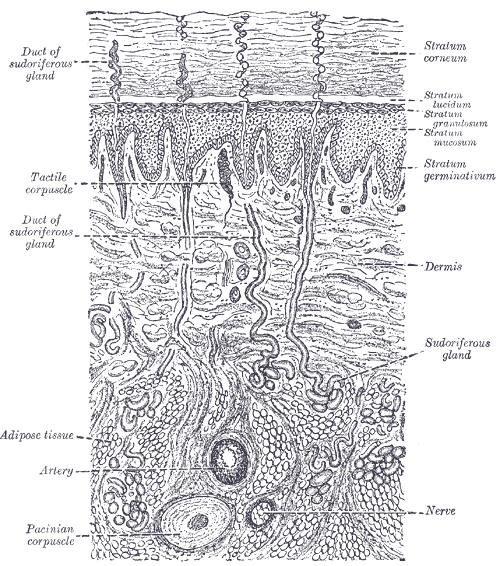
\includegraphics[width=0.7\linewidth]{./figures/sensation/Gray940} 

}

\caption{\href{https://commons.wikimedia.org/wiki/File:Skin.jpg}{Anatomy of human skin.}}\label{fig:skindiagram}
\end{figure}

\hypertarget{cutaneous-mechanoreceptors}{%
\subsection{Cutaneous Mechanoreceptors}\label{cutaneous-mechanoreceptors}}

Cutaneous mechanoreceptors respond to mechanical stimuli that result from physical interaction, including pressure and vibration. They are located in the skin. They are all innervated by Aβ fibers, except the mechanorecepting free nerve endings, which are Aδ fibers. Cutaneous mechanoreceptors can be categorized by morphology, by what kind of sensation they perceive, and by the rate of adaptation. Furthermore, each has a different receptive field.



\begin{figure}

{\centering 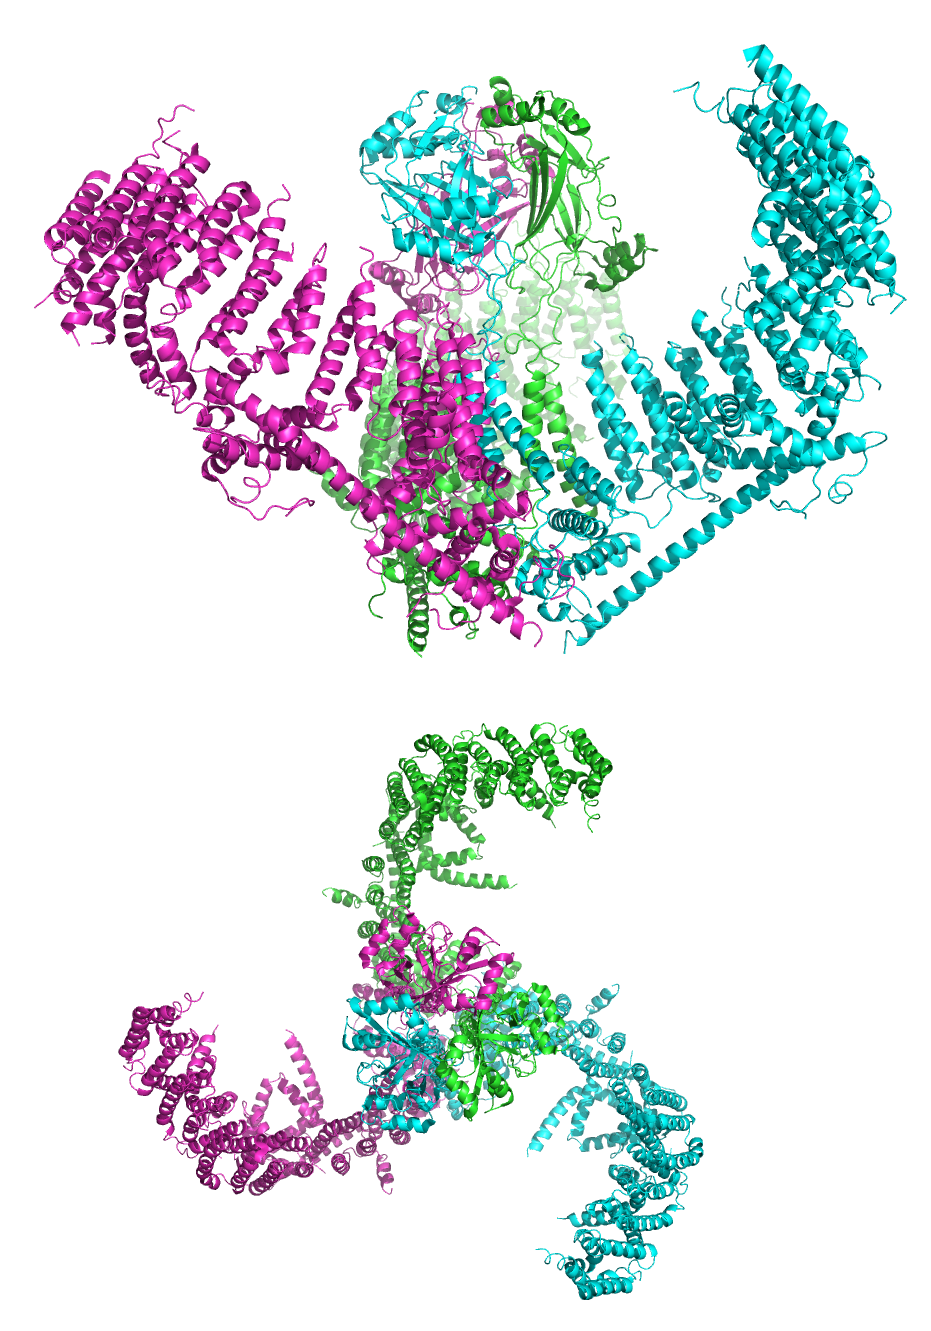
\includegraphics[width=0.7\linewidth]{./figures/sensation/mechano_sensitive_channel} 

}

\caption{A cartoon representation of the mechanosensitive Piezo1 channel in side and top view. \href{https://www.rcsb.org/structure/5Z10}{PDB 5Z10}, rendered with open source molecular visualization tool PyMol.}\label{fig:mechanosensitive}
\end{figure}

In the somatosensory system, receptive fields are regions of the skin or of internal organs. Some types of mechanoreceptors have large receptive fields, while others have smaller ones. Large receptive fields allow the cell to detect changes over a wider area, but lead to a less precise perception. Thus, the fingers, which require the ability to detect fine detail, have many, densely packed (up to 500 per cubic cm) mechanoreceptors with small receptive fields (around 10 square mm), while the back and legs, for example, have fewer receptors with large receptive fields.

Tactile-sense-related cortical neurons have receptive fields on the skin that can be modified by experience or by injury to sensory nerves resulting in changes in the field's size and position. In general these neurons have relatively large receptive fields (much larger than those of dorsal root ganglion cells). However, the neurons are able to discriminate fine detail due to patterns of excitation and inhibition relative to the field which leads to spatial resolution.

The term receptive field was first used by Sherrington (1906) to describe the area of skin from which a scratch reflex could be elicited in a dog. According to Alonso and Chen (2008) it was Hartline (1938) who applied the term to single neurons, in this case from the retina of a frog.

A sensory space can also map into a particular region on an animal's body. For example, it could be a hair in the cochlea or a piece of skin, retina, or tongue or other part of an animal's body.

This concept of receptive fields can be extended further up the nervous system; if many sensory receptors all form synapses with a single cell further up, they collectively form the receptive field of that cell. For example, the receptive field of a ganglion cell in the retina of the eye is composed of input from all of the photoreceptors which synapse with it, and a group of ganglion cells in turn forms the receptive field for a cell in the brain. This process is called convergence.

Tactile corpuscles or Meissner's corpuscles are a type of mechanoreceptor discovered by anatomist \href{https://en.wikipedia.org/wiki/Georg_Meissner}{Georg Meissner} (1829--1905) and \href{https://en.wikipedia.org/wiki/Rudolf_Wagner}{Rudolf Wagner}. They are a type of nerve ending in the skin that is responsible for sensitivity to light touch. In particular, they have their highest sensitivity (lowest threshold) when sensing vibrations between 10 and 50 hertz. They are rapidly adaptive receptors. They are most concentrated in thick hairless skin, especially at the finger pads.

Tactile corpuscles are encapsulated myelinated nerve endings, which consist of flattened supportive cells arranged as horizontal lamellae surrounded by a connective tissue capsule. The corpuscle is 30--140 μm in length and 40--60 μm in diameter. A single nerve fiber meanders between the lamellae and throughout the corpuscle.

Pacinian corpuscles (or lamellar corpuscles; discovered by Italian anatomist \href{https://en.wikipedia.org/wiki/Filippo_Pacini}{Filippo Pacini}) are one of the four major types of mechanoreceptor cell in glabrous (hairless) mammalian skin. They are nerve endings in the skin responsible for sensitivity to vibration and pressure. They respond only to sudden disturbances and are especially sensitive to vibration. The vibrational role may be used to detect surface texture, e.g., rough vs.~smooth. Pacinian corpuscles are also found in the pancreas, where they detect vibration and possibly very low frequency sounds.{[}dubious -- discuss{]} Pacinian corpuscles act as very rapidly adapting mechanoreceptors. Groups of corpuscles respond to pressure changes, e.g.~on grasping or releasing an object.

Pacinian corpuscles are larger and fewer in number than Meissner's corpuscle, Merkel cells and Ruffini's corpuscles.

The Pacinian corpuscle is approximately oval-cylindrical-shaped and 1 mm in length. The entire corpuscle is wrapped by a layer of connective tissue. Its capsule consists of 20 to 60 concentric lamellae (hence the alternative lamellar corpuscle) including fibroblasts and fibrous connective tissue (mainly Type IV and Type II collagen network), separated by gelatinous material, more than 92\% of which is water.

Pacinian corpuscles are rapidly adapting (phasic) receptors that detect gross pressure changes and vibrations in the skin. Any deformation in the corpuscle causes action potentials to be generated by opening pressure-sensitive sodium ion channels in the axon membrane. This allows sodium ions to influx, creating a receptor potential.

These corpuscles are especially susceptible to vibrations, which they can sense even centimeters away. Their optimal sensitivity is 250 Hz, and this is the frequency range generated upon fingertips by textures made of features smaller than 1 µm. Pacinian corpuscles cause action potentials when the skin is rapidly indented but not when the pressure is steady, due to the layers of connective tissue that cover the nerve ending. It is thought that they respond to high-velocity changes in joint position. They have also been implicated in detecting the location of touch sensations on handheld tools.

Pacinian corpuscles have a large receptive field on the skin's surface with an especially sensitive center.

Merkel cells, also known as Merkel-Ranvier cells or tactile epithelial cells, are oval-shaped mechanoreceptors essential for light touch sensation and found in the skin of vertebrates. They are abundant in highly sensitive skin like that of the fingertips in humans, and make synaptic contacts with somatosensory afferent nerve fibers. Although uncommon, these cells may become malignant and form a Merkel cell carcinoma---an aggressive and difficult to treat skin cancer.

Though it has been reported that Merkel cells are derived from neural crest cells, more recent experiments in mammals have indicated that they are in fact epithelial in origin.



\begin{figure}

{\centering 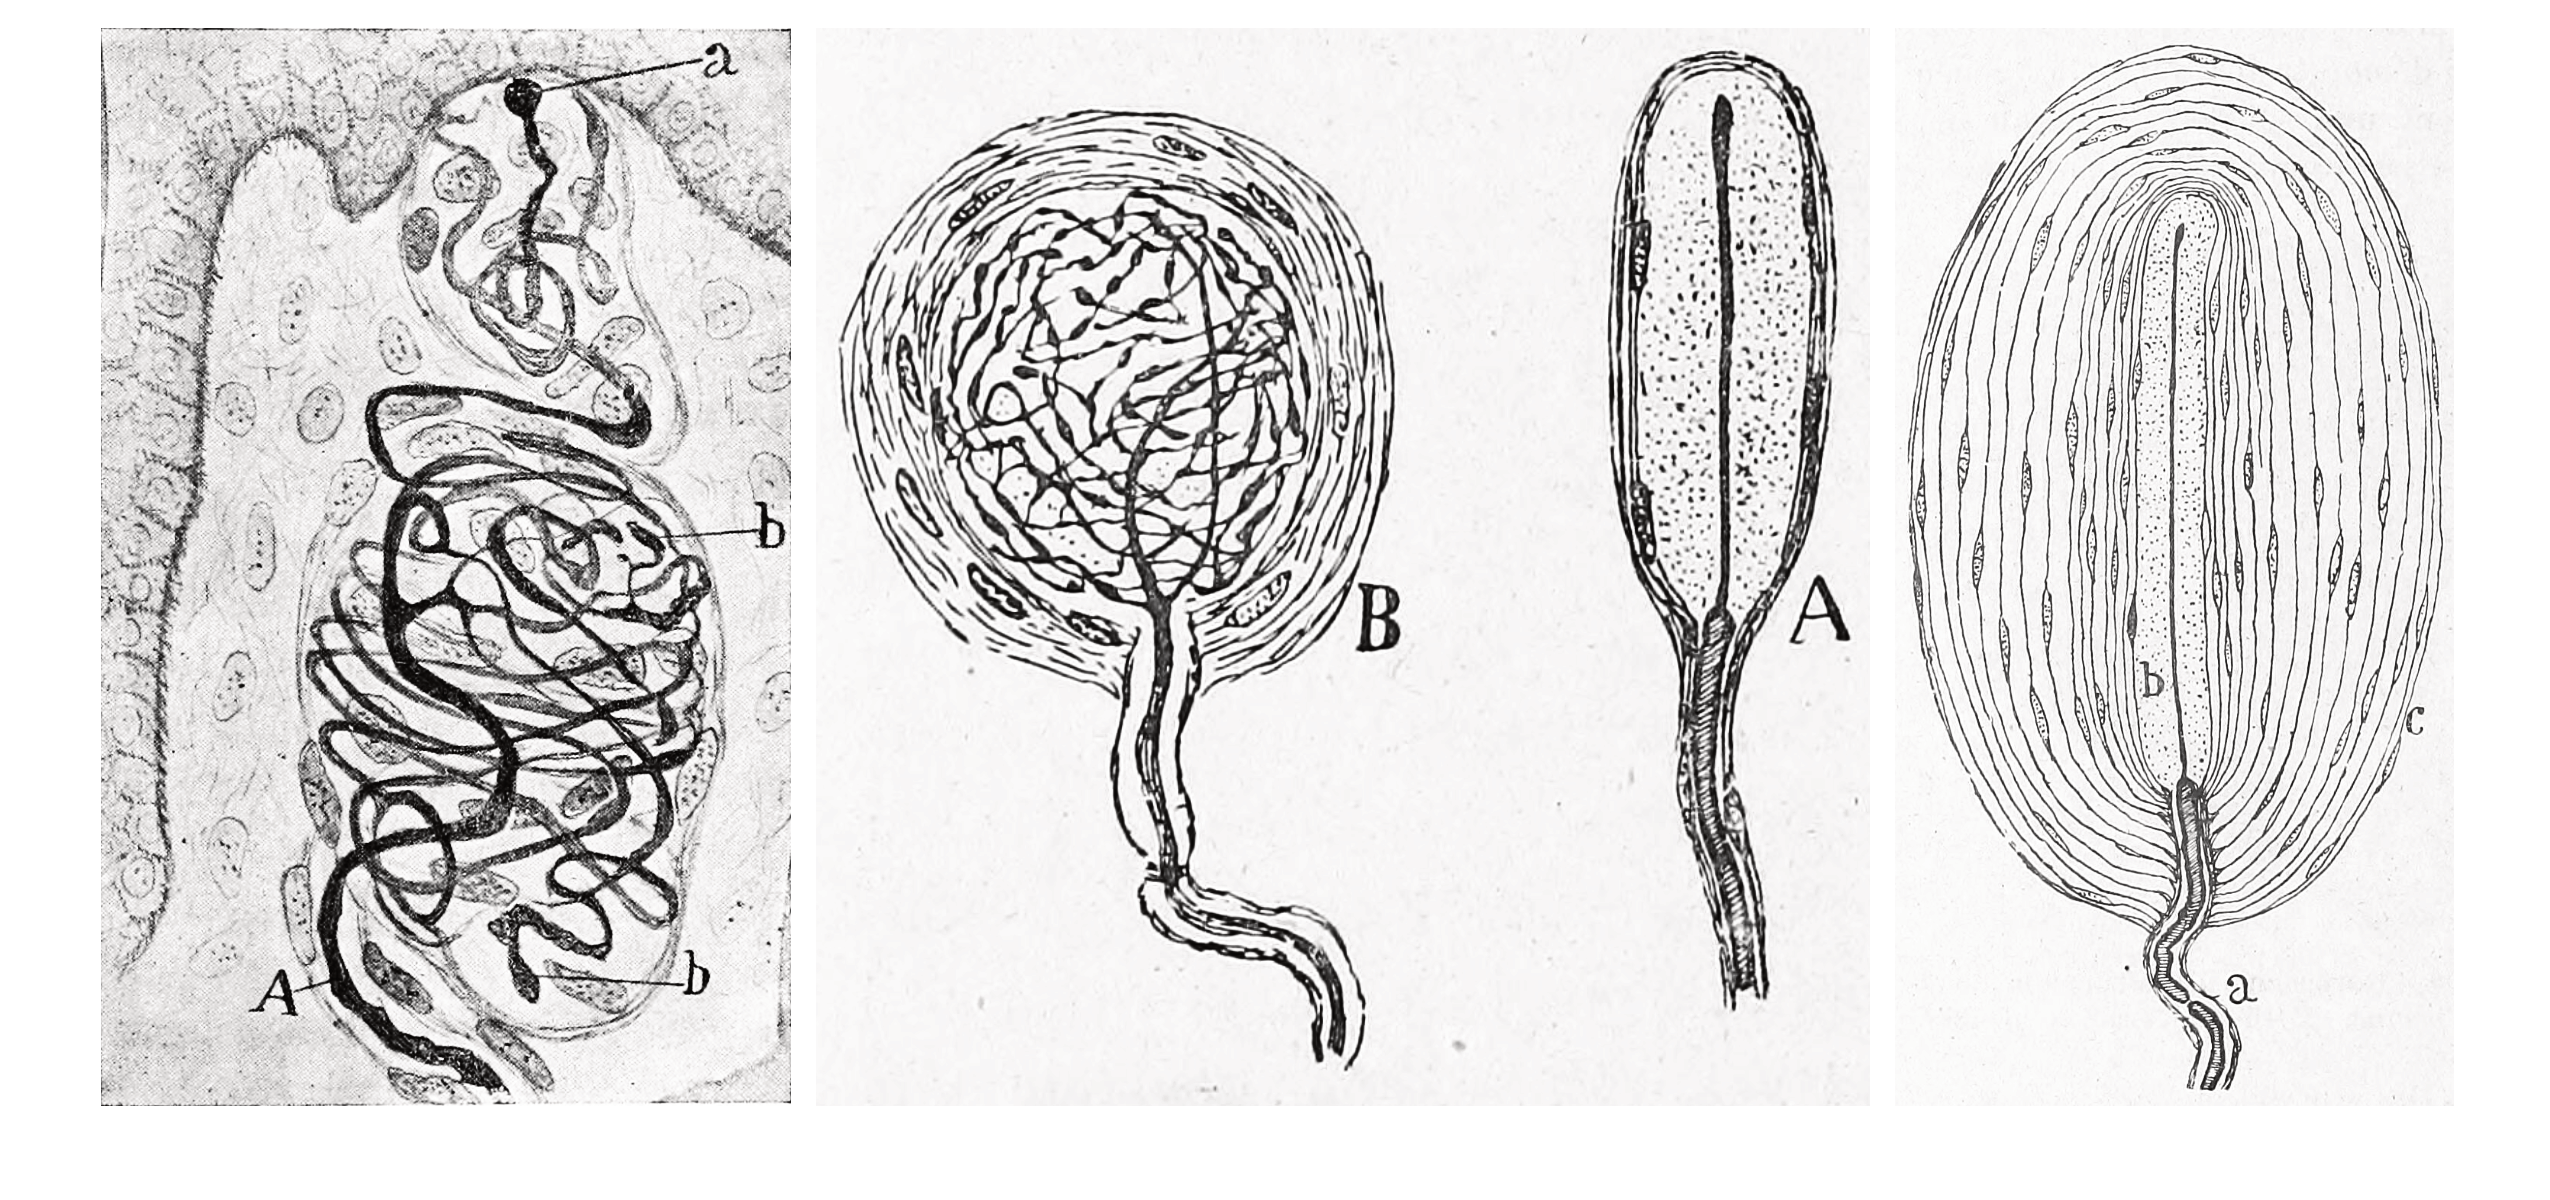
\includegraphics[width=0.7\linewidth]{./figures/sensation/TouchReceptors} 

}

\caption{\href{https://commons.wikimedia.org/wiki/File:Gray940.png}{Tactile corpuscles (from left to right): Meissner, Krause, Pacini}}\label{fig:tactilecorpuscle}
\end{figure}

Merkel cells are found in the skin and some parts of the mucosa of all vertebrates. In mammalian skin, they are clear cells found in the stratum basale (at the bottom of sweat duct ridges) of the epidermis approximately 10 μm in diameter. They also occur in epidermal invaginations of the plantar foot surface called rete ridges. Most often, they are associated with sensory nerve endings, when they are known as Merkel nerve endings (also called a Merkel cell-neurite complex). They are associated with slowly adapting (SA1) somatosensory nerve fibers. They react to low vibrations (5--15 Hz) and deep static touch such as shapes and edges. Due to a small receptive field (extremely detailed info) they are used in areas like fingertips the most; they are not covered (shelled) and thus respond to pressures over long periods.

The German anatomist \href{https://en.wikipedia.org/wiki/Friedrich_Sigmund_Merkel}{Friedrich Sigmund Merkel} referred to these cells as Tastzellen or ``touch cells'' but this proposed function has been controversial as it has been hard to prove. Though, genetic knockout mice have recently shown that Merkel cells are essential for the specialized coding by which afferent nerves resolve fine spatial details. Merkel cells are sometimes considered APUD cells (an older definition. More commonly classified as a part of dispersed neuroendocrine system) because they contain dense core granules, and thus may also have a neuroendocrine function.

The bulboid corpuscles (end-bulbs of Krause) are cutaneous receptors in the human body. The end-bulbs of Krause were named after the German anatomist \href{https://en.wikipedia.org/wiki/Wilhelm_Krause}{Wilhelm Krause} (1833--1910). End-bulbs are found in the conjunctiva of the eye (where they are spheroidal in shape in humans, but cylindrical in most other animals), in the mucous membrane of the lips and tongue, and in the epineurium of nerve trunks. They are also found in the penis and the clitoris and have received the name of genital corpuscles. The end-bulbs of Krause were thought to be thermoreceptors, sensing cold temperatures, but their function is unknown.

The Bulbous corpuscle or Ruffini ending or Ruffini corpuscle is a slowly adapting mechanoreceptor located in the cutaneous tissue between the dermal papillae and the hypodermis. It is named after Angelo Ruffini.

Ruffini corpuscles are enlarged dendritic endings with elongated capsules.

This spindle-shaped receptor is sensitive to skin stretch, and contributes to the kinesthetic sense of and control of finger position and movement. They are at the highest density around the fingernails where they act in monitoring slippage of objects along the surface of the skin, allowing modulation of grip on an object.

Ruffini corpuscles respond to sustained pressure and show very little adaptation.

Ruffinian endings are located in the deep layers of the skin, and register mechanical deformation within joints, more specifically angle change, with a specificity of up to 2.75 degrees, as well as continuous pressure states. They also act as thermoreceptors that respond for a long time, so in case of deep burn there will be pain, as these receptors will be burned off.

\hypertarget{nociception}{%
\subsection{Nociception}\label{nociception}}

\href{https://en.wikipedia.org/wiki/Nociception}{Nociception} (also nocioception or nociperception, from Latin nocere `to harm or hurt') is the sensory nervous system's response to certain harmful or potentially harmful stimuli. The term ``nociception'' was coined by \href{https://en.wikipedia.org/wiki/Charles_Scott_Sherrington}{Charles Scott Sherrington} to distinguish the physiological process (nervous activity) from pain (a subjective experience). In nociception, intense chemical (e.g., cayenne powder), mechanical (e.g., cutting, crushing), or thermal (heat and cold) stimulation of sensory nerve cells called nociceptors produces a signal that travels along a chain of nerve fibers via the spinal cord to the brain. Nociception triggers a variety of physiological and behavioral responses and usually results in a subjective experience of pain in sentient beings. Nociception can also cause generalized autonomic responses before or without reaching consciousness to cause pallor, sweating, tachycardia, hypertension, lightheadedness, nausea and fainting.

Potentially damaging mechanical, thermal, and chemical stimuli are detected by nerve endings called nociceptors, which are found in the skin, on internal surfaces such as the periosteum, joint surfaces, and in some internal organs. Some nociceptors are unspecialized free nerve endings that have their cell bodies outside the spinal column in the dorsal root ganglia. Nociceptors are categorized according to the axons which travel from the receptors to the spinal cord or brain.

Nociceptors have a certain threshold; that is, they require a minimum intensity of stimulation before they trigger a signal. Once this threshold is reached a signal is passed along the axon of the neuron into the spinal cord.

Nociceptive threshold testing deliberately applies a noxious stimulus to a human or animal subject in order to study pain. In animals, the technique is often used to study the efficacy of analgesic drugs and to establish dosing levels and period of effect. After establishing a baseline, the drug under test is given and the elevation in threshold recorded at specified time points. When the drug wears off, the threshold should return to the baseline (pre-treatment) value.

In some conditions, excitation of pain fibers becomes greater as the pain stimulus continues, leading to a condition called hyperalgesia.

Thermoception refers to stimuli of moderate temperatures 24--28 °C (75--82 °F), as anything beyond that range is considered pain and moderated by nociceptors. TRP and potassium channels {[}TRPM (1-8), TRPV (1-6), TRAAK, and TREK{]} each respond to different temperatures (among other stimuli) which create action potentials in nerves which join the mechano (touch) system in the posterolateral tract. Thermoception, like proprioception, is then covered by the somatosensory system.

TRP channels that detect noxious stimuli (mechanical, thermal, and chemical pain) relay that info to nociceptors that generate an action potential. Mechanical TRP channels react to depression of their cells (like touch), thermal TRP change shape in different temperatures, and chemical TRP act like taste buds, signalling if their receptors bond to certain elements/chemicals.



\begin{figure}

{\centering 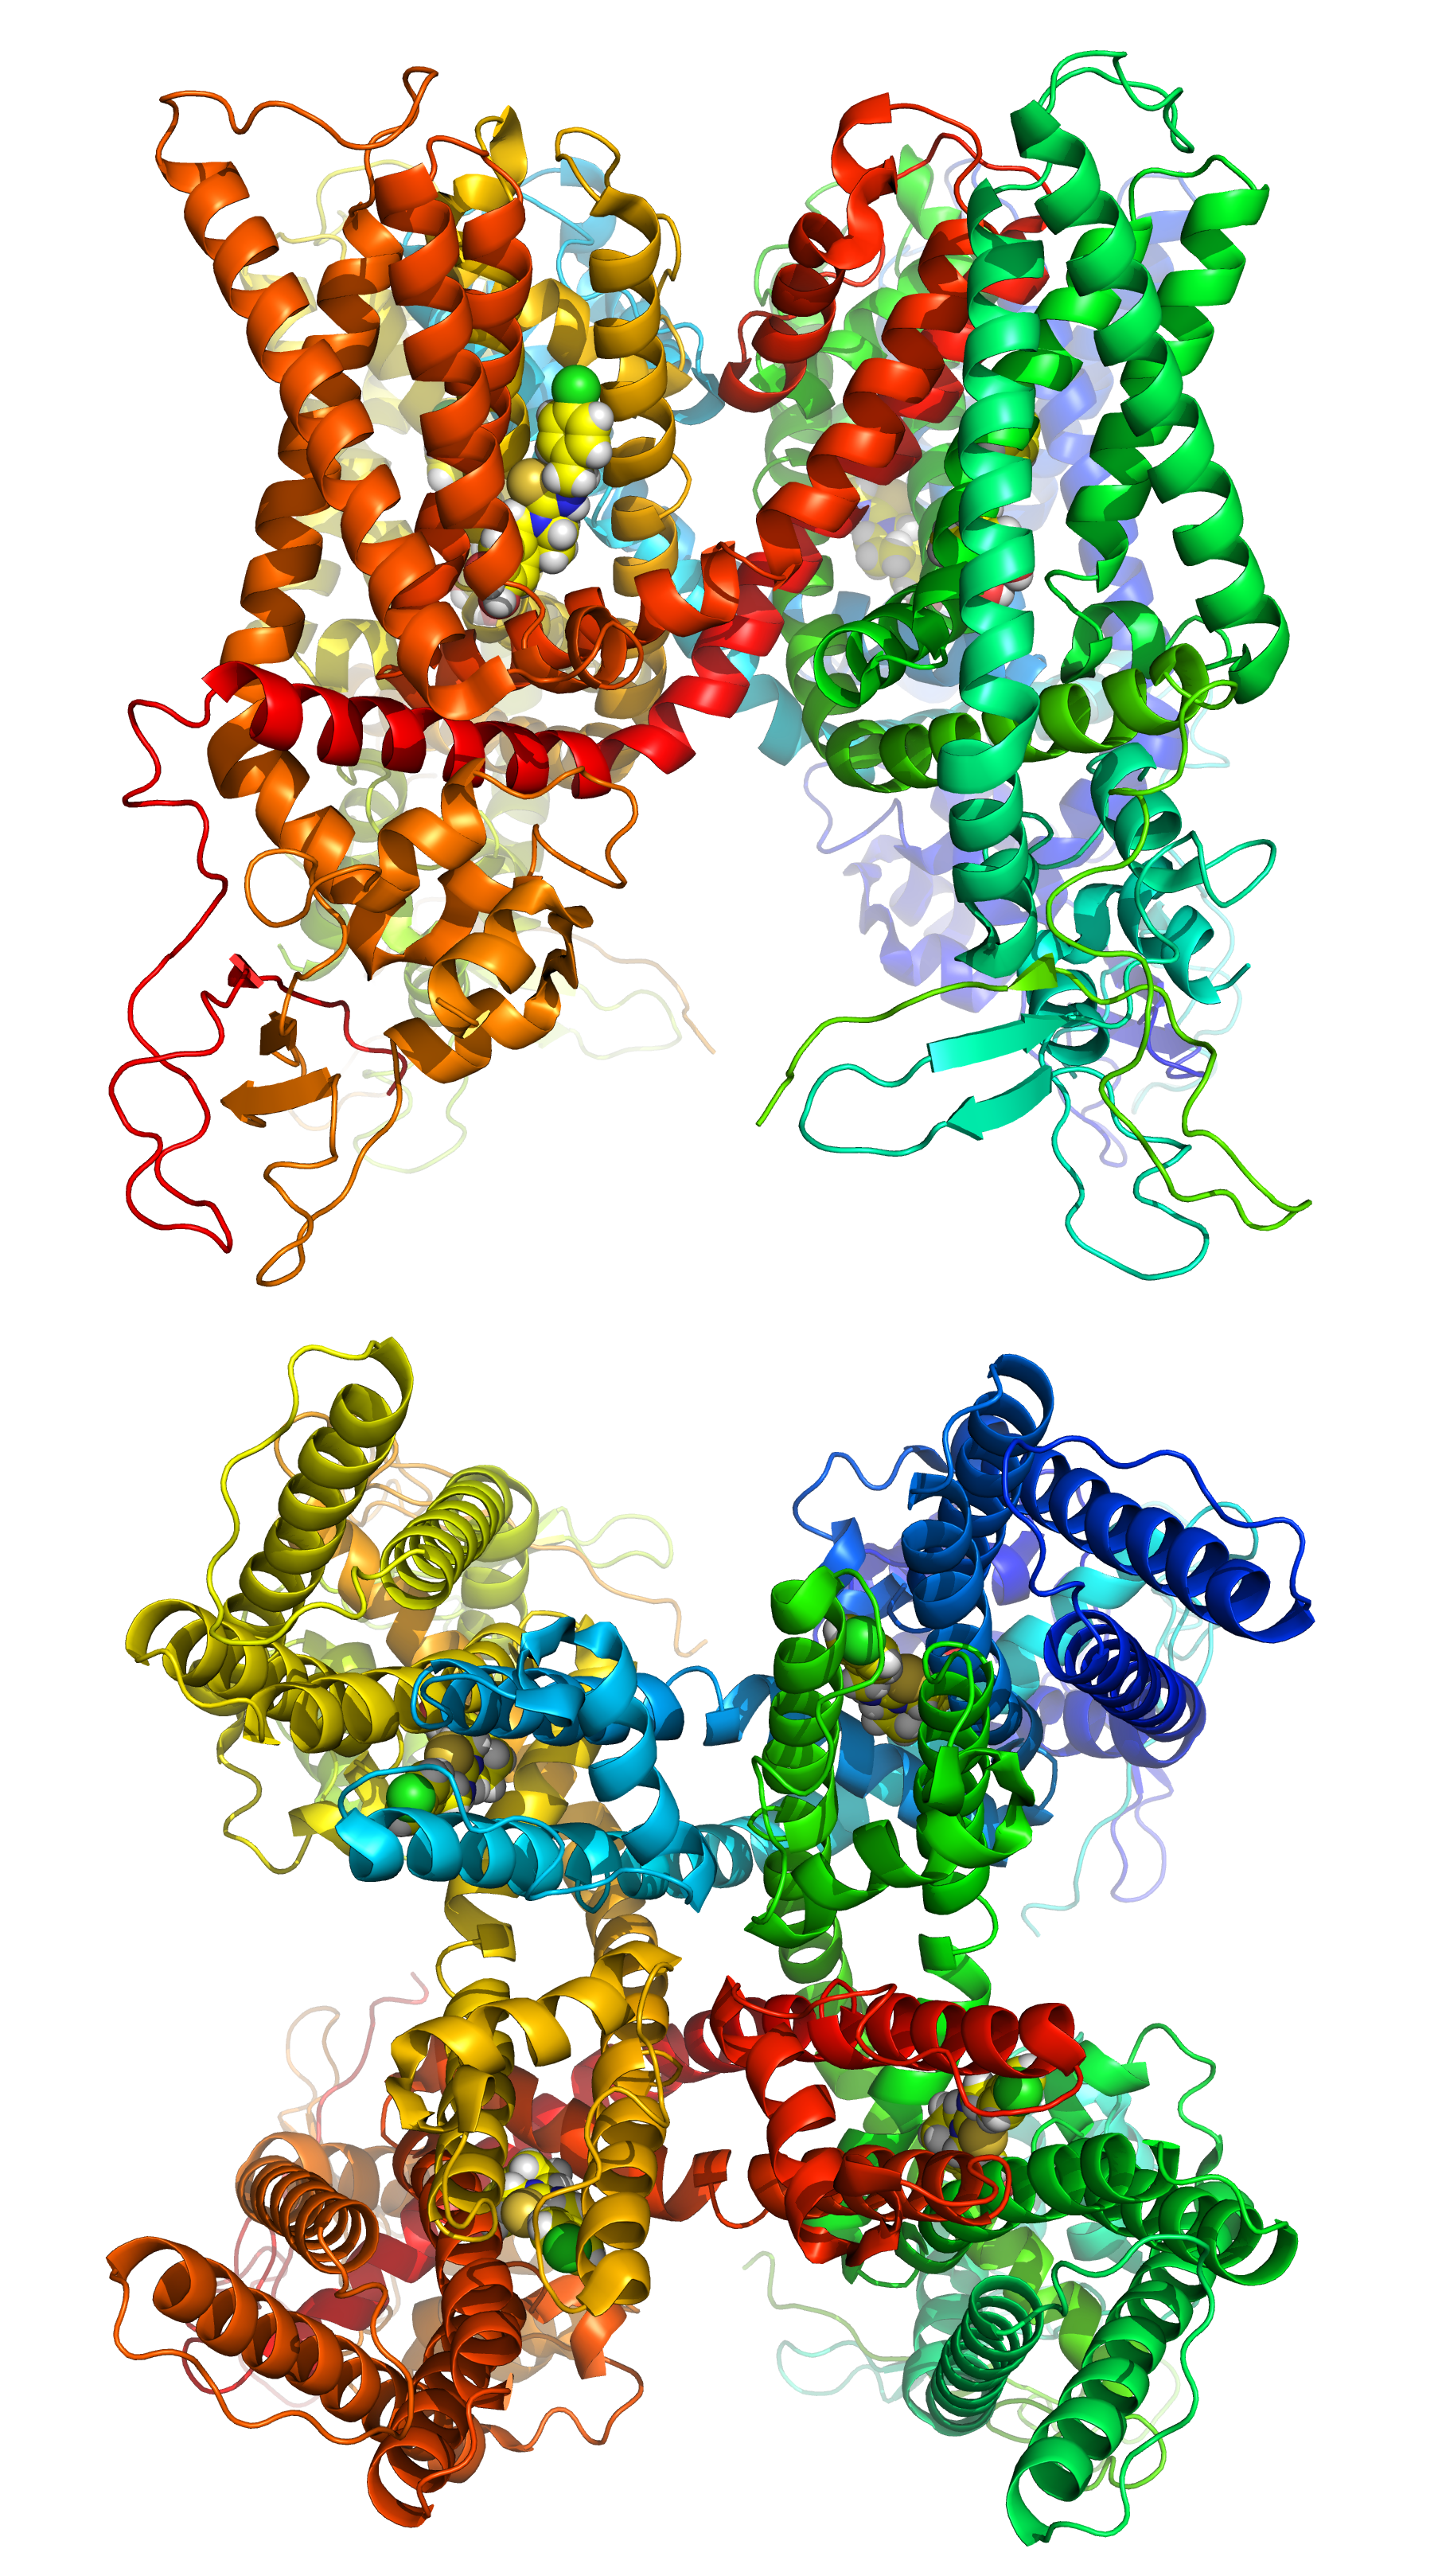
\includegraphics[width=0.7\linewidth]{./figures/sensation/TRPV1} 

}

\caption{A cartoon representation of the transient receptor potential cation channel subfamily V member 1 (TRPV1), also known as the capsaicin receptor and the vanilloid receptor 1 viewd from the side and the top. The function of TRPV1 is detection and regulation of body temperature. In addition, TRPV1 provides a sensation of scalding heat and pain (nociception). In primary afferent sensory neurons, it cooperates with TRPA1 (a chemical irritant receptor) to mediate the detection of noxious environmental stimuli. \href{https://www.rcsb.org/structure/5IS0}{PDB 5IS0}, rendered with open source molecular visualization tool PyMol.}\label{fig:TRPV1channel}
\end{figure}

\hypertarget{proprioception}{%
\subsection{Proprioception}\label{proprioception}}

Proprioception is the sense of self-movement and body position. It is sometimes described as the ``sixth sense''.

Proprioception is mediated by mechanically sensitive proprioceptor neurons distributed throughout an animal's body. Most vertebrates possess three basic types of proprioceptors: muscle spindles, which are embedded in skeletal muscle fibers, Golgi tendon organs, which lie at the interface of muscles and tendons, and joint receptors, which are low-threshold mechanoreceptors embedded in joint capsules. Many invertebrates, such as insects, also possess three basic proprioceptor types with analogous functional properties: chordotonal neurons, campaniform sensilla, and hair plates.

The initiation of proprioception is the activation of a proprioreceptor in the periphery. The proprioceptive sense is believed to be composed of information from sensory neurons located in the inner ear (motion and orientation) and in the stretch receptors located in the muscles and the joint-supporting ligaments (stance). There are specific nerve receptors for this form of perception termed ``proprioreceptors''.

An important role for proprioception is to allow an animal to stabilize itself against perturbations. For instance, for a person to walk or stand upright, they must continuously monitor their posture and adjust muscle activity as needed to provide balance. Similarly, when walking on unfamiliar terrain or even tripping, the person must adjust the output of their muscles quickly based on estimated limb position and velocity. Proprioceptor reflex circuits are thought to play an important role to allow fast and unconscious execution of these behaviors, To make control of these behaviors efficient, proprioceptors are also thought to regulate reciprocal inhibition in muscles, leading to agonist-antagonist muscle pairs.

When planning complex movements such as reaching or grooming, animals must consider the current position and velocity of their limb and use it to adjust dynamics to target a final position. If the animal's estimate of their limb's initial position is wrong, this can lead to a deficiency in the movement. Furthermore, proprioception is crucial in refining the movement if it deviates from the trajectory.

\hypertarget{muscle-spindles}{%
\subsection{Muscle Spindles}\label{muscle-spindles}}

Muscle spindles are stretch receptors within the body of a muscle that primarily detect changes in the length of the muscle. They convey length information to the central nervous system via afferent nerve fibers. This information can be processed by the brain as proprioception. The responses of muscle spindles to changes in length also play an important role in regulating the contraction of muscles, for example, by activating motor neurons via the stretch reflex to resist muscle stretch.



\begin{figure}

{\centering 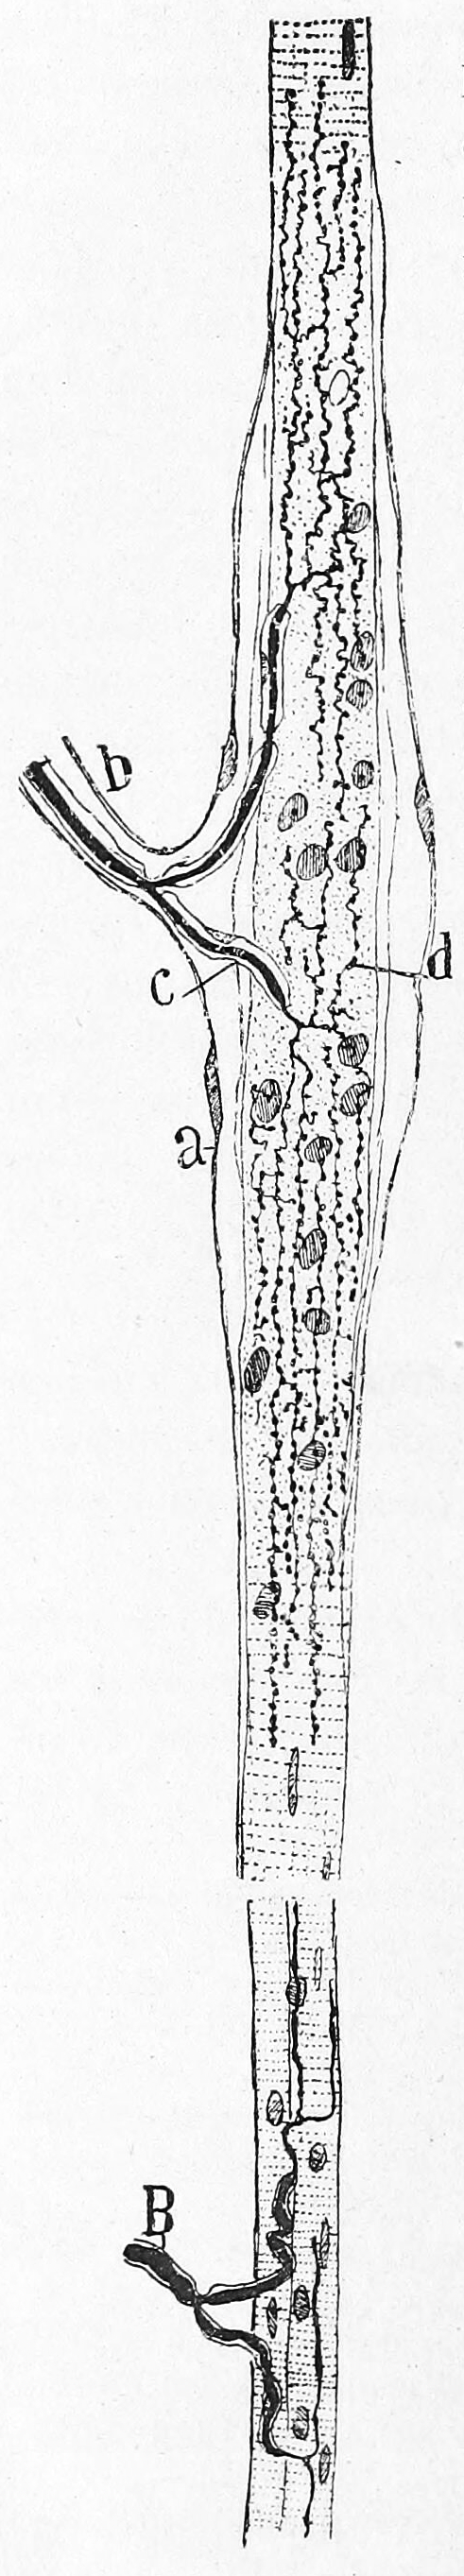
\includegraphics[width=0.7\linewidth]{./figures/sensation/CajalMuscleSpindle} 

}

\caption{Muscle spindle from the pectoral muscle of a frog. Bottom part of figure: B) extrafusal muscle fibers with efferent motor nerve; top part of figure: myelinated afferent nerve fiber. \href{https://wellcomelibrary.org/item/b2129592x\#?c=0\&m=0\&s=0\&cv=14\&z=0\%2C-3.48\%2C1\%2C8.6591}{Histologie du système nerveux de l'homme \& des vertébrés, Tome Premier} (1909) by Santiago Ramón y Cajal translated from Spanish by Dr.~L. Azoulay.}\label{fig:musclespindle}
\end{figure}

Muscle spindles are found within the belly of muscles, between extrafusal muscle fibers.{[}b{]} The specialised fibers that constitute the muscle spindle are known as intrafusal fibers (as they are present within the spindle), to distinguish themselves from the fibres of the muscle itself which are called extrafusal fibers. Muscle spindles have a capsule of connective tissue, and run parallel to the extrafusal muscle fibers.

\hypertarget{golgi-tendon-organ}{%
\subsection{Golgi Tendon Organ}\label{golgi-tendon-organ}}

The Golgi tendon organ (GTO) (also called Golgi organ, tendon organ, neurotendinous organ or neurotendinous spindle) is a proprioceptive sensory receptor organ that senses changes in muscle tension. It lies at the origins and insertion of skeletal muscle fibers into the tendons of skeletal muscle. It provides the sensory component of the Golgi tendon reflex.



\begin{figure}

{\centering 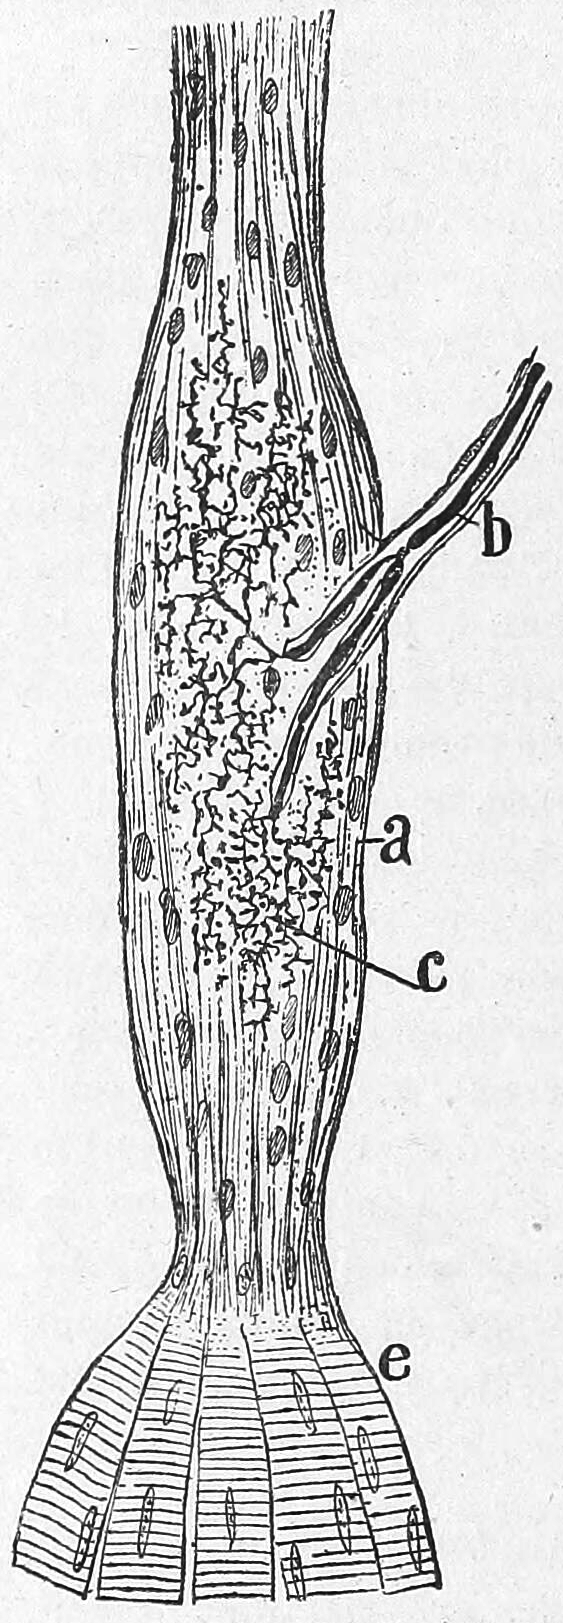
\includegraphics[width=0.7\linewidth]{./figures/sensation/CajalGolgiTendon} 

}

\caption{Golgi tendon organ from an adult cat. a) Termninal arboriasation and c) fine ultimate brances of the afferent nerve; b) myelinated afferent nerve fiber; e) muscle fibers. \href{https://wellcomelibrary.org/item/b2129592x\#?c=0\&m=0\&s=0\&cv=14\&z=0\%2C-3.48\%2C1\%2C8.6591}{Histologie du système nerveux de l'homme \& des vertébrés, Tome Premier} (1909) by Santiago Ramón y Cajal translated from Spanish by Dr.~L. Azoulay.}\label{fig:tendonorgan}
\end{figure}

The body of the organ is made up of braided strands of collagen (intrafusal fasciculi) that are less compact than elsewhere in the tendon and are encapsulated. The capsule is connected in series with a group of muscle fibers (10-20 fibers) at one end, and merge into the tendon proper at the other. Each capsule is about 1 mm long, has a diameter of about 0.1 mm, and is perforated by one or more afferent type Ib sensory nerve fibers (Aɑ fiber), which are large (12-20 μm) myelinated axons that can conduct nerve impulses very rapidly. Inside the capsule, the afferent fibers lose their medullary sheaths, branch, intertwine with the collagen fibers, and terminate as flattened leaf-like endings between the collagen strands (see figure).

\hypertarget{the-somatosensory-pathways}{%
\subsection{The Somatosensory Pathways}\label{the-somatosensory-pathways}}

All afferent touch/vibration info ascends the spinal cord via the posterior (dorsal) column-medial lemniscus pathway via gracilis (T7 and below) or cuneatus (T6 and above). Cuneatus sends signals to the cochlear nucleus indirectly via spinal grey matter, this info is used in determining if a perceived sound is just villi noise/irritation. All fibers cross (left becomes right) in the medulla.

A somatosensory pathway will typically have three neurons: first-order, second-order, and third-order.

\begin{enumerate}
\def\labelenumi{\arabic{enumi}.}
\tightlist
\item
  The first-order neuron is a type of pseudounipolar neuron and always has its cell body in the dorsal root ganglion of the spinal nerve with a peripheral axon innervating touch mechanoreceptors and a central axon synapsing on the second-order neuron. If the somatosensory pathway is in parts of the head or neck not covered by the cervical nerves, the first-order neuron will be the trigeminal nerve ganglia or the ganglia of other sensory cranial nerves).
\item
  The second-order neuron has its cell body either in the spinal cord or in the brainstem. This neuron's ascending axons will cross (decussate) to the opposite side either in the spinal cord or in the brainstem.
\item
  In the case of touch and certain types of pain, the third-order neuron has its cell body in the ventral posterior nucleus of the thalamus and ends in the postcentral gyrus of the parietal lobe in the primary somatosensory cortex (or S1).
\end{enumerate}

Fine touch (or discriminative touch) is a sensory modality that allows a subject to sense and localize touch. The form of touch where localization is not possible is known as crude touch. The posterior column--medial lemniscus pathway is the pathway responsible for the sending of fine touch information to the cerebral cortex of the brain.

Crude touch (or non-discriminative touch) is a sensory modality that allows the subject to sense that something has touched them, without being able to localize where they were touched (contrasting ``fine touch''). Its fibres are carried in the spinothalamic tract, unlike the fine touch, which is carried in the dorsal column. As fine touch normally works in parallel to crude touch, a person will be able to localize touch until fibres carrying fine touch (Posterior column--medial lemniscus pathway) have been disrupted. Then the subject will feel the touch, but be unable to identify where they were touched.

In humans, temperature sensation from thermoreceptors enters the spinal cord along the axons of Lissauer's tract that synapse on second order neurons in grey matter of the dorsal horn. The axons of these second order neurons then decussate, joining the spinothalamic tract as they ascend to neurons in the ventral posterolateral nucleus of the thalamus.

\hypertarget{the-primary-somatosensory-cortex}{%
\subsection{The Primary Somatosensory Cortex}\label{the-primary-somatosensory-cortex}}

The primary somatosensory cortex is located in the postcentral gyrus, and is part of the somatosensory system.

At the primary somatosensory cortex, tactile representation is orderly arranged (in an inverted fashion) from the toe (at the top of the cerebral hemisphere) to mouth (at the bottom). However, some body parts may be mapped to partially overlapping regions of cortex. Each cerebral hemisphere of the primary somatosensory cortex only contains a tactile representation of the opposite (contralateral) side of the body. The amount of primary somatosensory cortex devoted to a body part is not proportional to the absolute size of the body surface, but, instead, to the relative density of cutaneous tactile receptors on that body part. The density of cutaneous tactile receptors on a body part is generally indicative of the degree of sensitivity of tactile stimulation experienced at said body part. For example, the human lips and hands have a larger representation than other body parts.

Brodmann areas 3, 1, and 2 make up the primary somatosensory cortex of the human brain (or S1). Brodmann area (BA) 3 is subdivided into areas 3a and 3b. Because Brodmann sliced the brain somewhat obliquely, he encountered area 1 first; however, from anterior to posterior, the Brodmann designations are 3, 1, and 2, respectively.

Areas 1 and 2 receive dense inputs from BA 3b. The projection from 3b to 1 primarily relays texture information; the projection to area 2 emphasizes size and shape. Lesions confined to these areas produce predictable dysfunction in texture, size, and shape discrimination.

Somatosensory cortex, like other neocortex, is layered. Like other sensory cortex (i.e., visual and auditory) the thalamic inputs project into layer IV, which in turn project into other layers. As in other sensory cortices, S1 neurons are grouped together with similar inputs and responses into vertical columns that extend across cortical layers.

\hypertarget{the-olfactory-system}{%
\section{The Olfactory System}\label{the-olfactory-system}}

The olfactory system, or sense of smell, is the sensory system used for smelling (olfaction). Olfaction is one of the special senses, that have directly associated specific organs. Most mammals and reptiles have a main olfactory system and an accessory olfactory system. The main olfactory system detects airborne substances, while the accessory system senses fluid-phase stimuli. Often, land organisms will have separate olfaction systems for smell and taste (orthonasal smell and retronasal smell), but water-dwelling organisms usually have only one system. The senses of smell and taste (gustatory system) are often referred to together as the chemosensory system, because they both give the brain information about the chemical composition of objects.

Olfaction is a chemoreception that forms the sense of smell. Olfaction has many purposes, such as the detection of hazards, pheromones, and food. It integrates with other senses to form the sense of flavor. Olfaction occurs when odorants bind to specific sites on olfactory receptors located in the nasal cavity. Glomeruli aggregate signals from these receptors and transmit them to the olfactory bulb, where the sensory input will start to interact with parts of the brain responsible for smell identification, memory, and emotion.

In insects, smells are sensed by olfactory sensory neurons in the chemosensory sensilla, which are present in insect antenna, palps, and tarsa, but also on other parts of the insect body. Odorants penetrate into the cuticle pores of chemosensory sensilla and get in contact with insect odorant-binding proteins (OBPs) or Chemosensory proteins (CSPs), before activating the sensory neurons.

In vertebrates, smells are sensed by olfactory sensory neurons in the olfactory epithelium. The olfactory epithelium is made up of at least six morphologically and biochemically different cell types. The proportion of olfactory epithelium compared to respiratory epithelium (not innervated, or supplied with nerves) gives an indication of the animal's olfactory sensitivity. Humans have about 10 cm\textsuperscript{2} of olfactory epithelium, whereas some dogs have 170 cm\textsuperscript{2}. A dog's olfactory epithelium is also considerably more densely innervated, with a hundred times more receptors per square centimeter.

Molecules of odorants passing through the superior nasal concha of the nasal passages dissolve in the mucus that lines the superior portion of the cavity and are detected by olfactory receptors on the dendrites of the olfactory sensory neurons. This may occur by diffusion or by the binding of the odorant to odorant-binding proteins. The mucus overlying the epithelium contains mucopolysaccharides, salts, enzymes, and antibodies (these are highly important, as the olfactory neurons provide a direct passage for infection to pass to the brain). This mucus acts as a solvent for odor molecules, flows constantly, and is replaced approximately every ten minutes.

\hypertarget{the-nose}{%
\subsection{The Nose}\label{the-nose}}

The human nose is the most protruding part of the face. It bears the nostrils and is the first organ of the respiratory system. It is also the principal organ in the olfactory system. The shape of the nose is determined by the nasal bones and the nasal cartilages, including the nasal septum which separates the nostrils and divides the nasal cavity into two.

The main function of the nose is respiration, and the nasal mucosa lining the nasal cavity and the paranasal sinuses carries out the necessary conditioning of inhaled air by warming and moistening it. Nasal conchae, shell-like bones in the walls of the cavities, play a major part in this process. Filtering of the air by nasal hair in the nostrils prevents large particles from entering the lungs. Sneezing is a reflex to expel unwanted particles from the nose that irritate the mucosal lining. Sneezing can transmit infections, because aerosols are created in which the droplets can harbour pathogens.

Another major function of the nose is olfaction, the sense of smell. The area of olfactory epithelium, in the upper nasal cavity, contains specialised olfactory cells responsible for this function.

The peripheral olfactory system consists mainly of the nostrils, ethmoid bone, nasal cavity, and the olfactory epithelium (layers of thin tissue covered in mucus that line the nasal cavity). The primary components of the layers of epithelial tissue are the mucous membranes, olfactory glands, olfactory neurons, and nerve fibers of the olfactory nerves.



\begin{figure}

{\centering 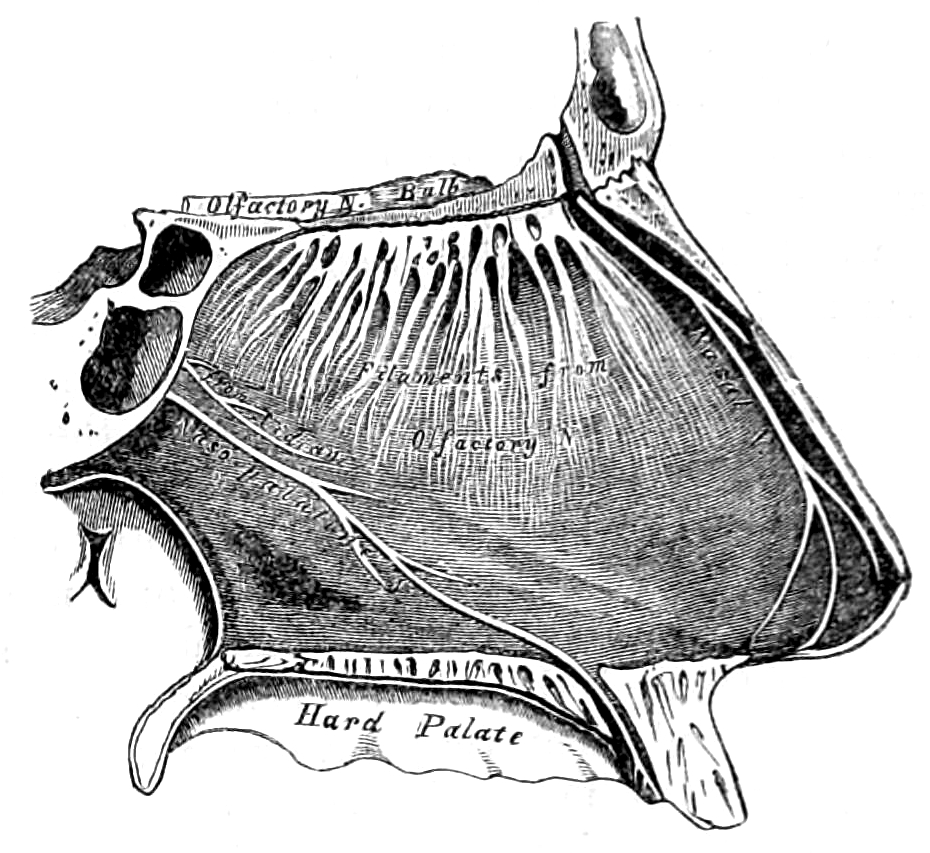
\includegraphics[width=0.7\linewidth]{./figures/sensation/GrayP572} 

}

\caption{View of the right side of the nasal septum showing the olfactory bulb and the filaments of the olfactory nerve.From \href{https://wellcomelibrary.org/item/b21688692}{Gray, Henry: Anatomy Descriptive And Surgical. 7\textsuperscript{th} Edition, Longmans, Green, And Co., London, 1875}.}\label{fig:rightseptum}
\end{figure}

Odor molecules can enter the peripheral pathway and reach the nasal cavity either through the nostrils when inhaling (olfaction) or through the throat when the tongue pushes air to the back of the nasal cavity while chewing or swallowing (retro-nasal olfaction). Inside the nasal cavity, mucus lining the walls of the cavity dissolves odor molecules. Mucus also covers the olfactory epithelium, which contains mucous membranes that produce and store mucus and olfactory glands that secrete metabolic enzymes found in the mucus.

\hypertarget{olfactory-sensory-neurons}{%
\subsection{Olfactory Sensory Neurons}\label{olfactory-sensory-neurons}}

Humans have between 10 and 20 million olfactory receptor neurons (ORNs). In vertebrates, ORNs are bipolar neurons with dendrites facing the external surface of the cribriform plate with axons that pass through the cribriform foramina with terminal end at olfactory bulbs. The ORNs are located in the olfactory epithelium in the nasal cavity. The cell bodies of the ORNs are distributed among all three of the stratified layers of the olfactory epithelium.

Many tiny hair-like cilia protrude from the olfactory receptor cell's dendrite into the mucus covering the surface of the olfactory epithelium. The surface of these cilia is covered with olfactory receptors, a type of G protein-coupled receptor. Each olfactory receptor cell expresses only one type of olfactory receptor (OR), but many separate olfactory receptor cells express ORs which bind the same set of odors. The axons of olfactory receptor cells which express the same OR converge to form glomeruli in the olfactory bulb.Olfactory sensory neurons in the epithelium detect odor molecules dissolved in the mucus and transmit information about the odor to the brain in a process called sensory transduction. Olfactory neurons have cilia (tiny hairs) containing olfactory receptors that bind to odor molecules, causing an electrical response that spreads through the sensory neuron to the olfactory nerve fibers at the back of the nasal cavity.

Olfactory receptors (ORs), also known as odorant receptors, are expressed in the cell membranes of olfactory receptor neurons and are responsible for the detection of odorants (i.e., compounds that have an odor) which give rise to the sense of smell. Activated olfactory receptors trigger nerve impulses which transmit information about odor to the brain. These receptors are members of the class A rhodopsin-like family of G protein-coupled receptors (GPCRs). The olfactory receptors form a multigene family consisting of around 800 genes in humans and 1400 genes in mice

Rather than binding specific ligands, olfactory receptors display affinity for a range of odor molecules, and conversely a single odorant molecule may bind to a number of olfactory receptors with varying affinities, which depend on physio-chemical properties of molecules like their molecular volumes. Once the odorant has bound to the odor receptor, the receptor undergoes structural changes and it binds and activates the olfactory-type G protein on the inside of the olfactory receptor neuron. The G protein (G\textsubscript{olf} and/or G\textsubscript{s}) in turn activates adenylate cyclase - which converts ATP into cyclic AMP (cAMP). The cAMP opens cyclic nucleotide-gated ion channels which allow calcium and sodium ions to enter into the cell, depolarizing the olfactory receptor neuron and triggering the firing of action potentials which convey the information to the brain.

Olfactory nerves and fibers transmit information about odors from the peripheral olfactory system to the central olfactory system of the brain, which is separated from the epithelium by the cribriform plate of the ethmoid bone. Olfactory nerve fibers, which originate in the epithelium, pass through the cribriform plate, connecting the epithelium to the brain's limbic system at the olfactory bulbs.



\begin{figure}

{\centering 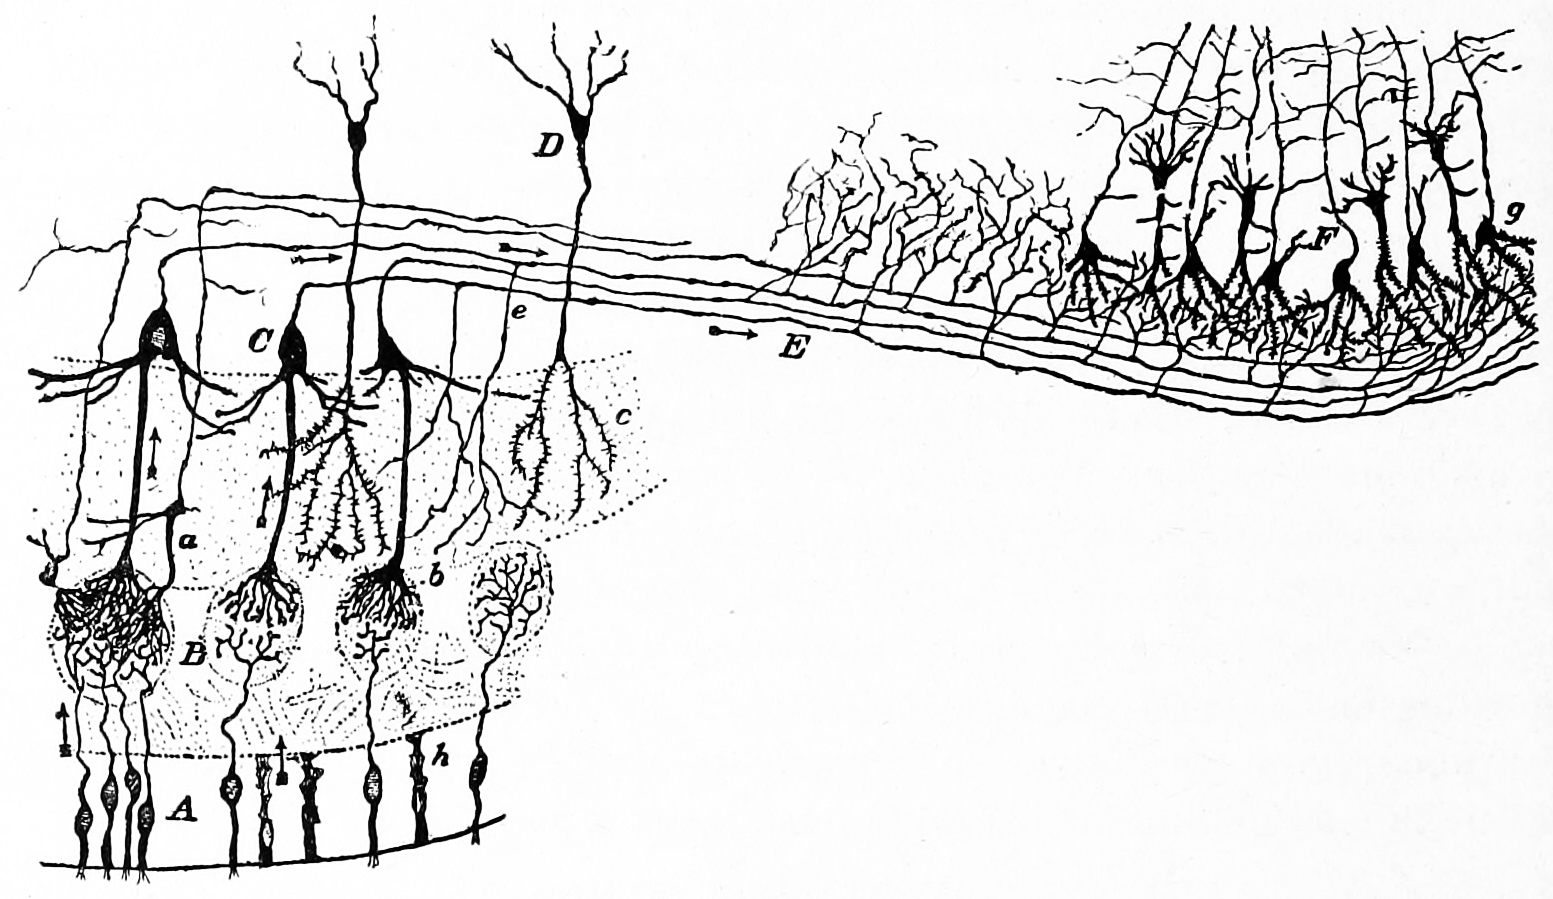
\includegraphics[width=0.7\linewidth]{./figures/sensation/CajalOlfactoryPathway} 

}

\caption{Diagram of the structure of the olfactory bulb and olfactory cortex. A) Olfacory mucosa; B) glomeruli in the olfactory bulb; C) mitral cells; D) granule cells; E) olfactory nerve; F) pyramidal cells in the olfactory cortex. Action potentials fired by the olfactory receptor cells and subsequently by the cells in the olfactory bulb, travel to the olfactory cortex (arrows). \href{https://wellcomelibrary.org/item/b2129592x\#?c=0\&m=0\&s=0\&cv=14\&z=0\%2C-3.48\%2C1\%2C8.6591}{Histologie du système nerveux de l'homme \& des vertébrés, Tome Premier} (1909) by Santiago Ramón y Cajal translated from Spanish by Dr.~L. Azoulay.}\label{fig:olfactory}
\end{figure}

\hypertarget{the-olfactory-bulb}{%
\subsection{The Olfactory Bulb}\label{the-olfactory-bulb}}

The main olfactory bulb transmits pulses to both mitral and tufted cells, which help determine odor concentration based off the time certain neuron clusters fire (called `timing code'). These cells also note differences between highly similar odors and use that data to aid in later recognition. The cells are different with mitral having low firing-rates and being easily inhibited by neighboring cells, while tufted have high rates of firing and are more difficult to inhibit.

\hypertarget{the-olfactory-cortex}{%
\subsection{The Olfactory Cortex}\label{the-olfactory-cortex}}

The uncus(an anterior extremity of the parahippocampal gyrus, a region that surrounds the hippocampus and is part of the limbic system) houses the olfactory cortex which includes the piriform cortex (posterior orbitofrontal cortex), amygdala, olfactory tubercle, and parahippocampal gyrus.

The olfactory tubercle connects to numerous areas of the amygdala, thalamus, hypothalamus, hippocampus, brain stem, retina, auditory cortex, and olfactory system.

The anterior olfactory nucleus distributes reciprocal signals between the olfactory bulb and piriform cortex. The anterior olfactory nucleus is the memory hub for smell.

\hypertarget{olfactory-pathways}{%
\subsection{Olfactory Pathways}\label{olfactory-pathways}}

Olfactory sensory neurons project axons to the brain within the olfactory nerve, (cranial nerve I). These nerve fibers, lacking myelin sheaths, pass to the olfactory bulb of the brain through perforations in the cribriform plate, which in turn projects olfactory information to the olfactory cortex and other areas. The axons from the olfactory receptors converge in the outer layer of the olfactory bulb within small (≈50 micrometers in diameter) structures called glomeruli. Mitral cells, located in the inner layer of the olfactory bulb, form synapses with the axons of the sensory neurons within glomeruli and send the information about the odor to other parts of the olfactory system, where multiple signals may be processed to form a synthesized olfactory perception. A large degree of convergence occurs, with 25,000 axons synapsing on 25 or so mitral cells, and with each of these mitral cells projecting to multiple glomeruli. Mitral cells also project to periglomerular cells and granular cells that inhibit the mitral cells surrounding it (lateral inhibition). Granular cells also mediate inhibition and excitation of mitral cells through pathways from centrifugal fibers and the anterior olfactory nuclei. Neuromodulators like acetylcholine, serotonin and norepinephrine all send axons to the olfactory bulb and have been implicated in gain modulation, pattern separation, and memory functions, respectively.

The mitral cells leave the olfactory bulb in the lateral olfactory tract, which synapses on five major regions of the cerebrum: the anterior olfactory nucleus, the olfactory tubercle, the amygdala, the piriform cortex, and the entorhinal cortex. The anterior olfactory nucleus projects, via the anterior commissure, to the contralateral olfactory bulb, inhibiting it. The piriform cortex has two major divisions with anatomically distinct organizations and functions. The anterior piriform cortex (APC) appears to be better at determining the chemical structure of the odorant molecules, and the posterior piriform cortex (PPC) has a strong role in categorizing odors and assessing similarities between odors (e.g.~minty, woody, and citrus are odors that can, despite being highly variant chemicals, be distinguished via the PPC in a concentration-independent manner). The piriform cortex projects to the medial dorsal nucleus of the thalamus, which then projects to the orbitofrontal cortex. The orbitofrontal cortex mediates conscious perception of the odor (citation needed). The three-layered piriform cortex projects to a number of thalamic and hypothalamic nuclei, the hippocampus and amygdala and the orbitofrontal cortex, but its function is largely unknown. The entorhinal cortex projects to the amygdala and is involved in emotional and autonomic responses to odor. It also projects to the hippocampus and is involved in motivation and memory. Odor information is stored in long-term memory and has strong connections to emotional memory. This is possibly due to the olfactory system's close anatomical ties to the limbic system and hippocampus, areas of the brain that have long been known to be involved in emotion and place memory, respectively.

Since any one receptor is responsive to various odorants, and there is a great deal of convergence at the level of the olfactory bulb, it may seem strange that human beings are able to distinguish so many different odors. It seems that a highly complex form of processing must be occurring; however, as it can be shown that, while many neurons in the olfactory bulb (and even the pyriform cortex and amygdala) are responsive to many different odors, half the neurons in the orbitofrontal cortex are responsive to only one odor, and the rest to only a few. It has been shown through microelectrode studies that each individual odor gives a particular spatial map of excitation in the olfactory bulb. It is possible that the brain is able to distinguish specific odors through spatial encoding, but temporal coding must also be taken into account. Over time, the spatial maps change, even for one particular odor, and the brain must be able to process these details as well.

Inputs from the two nostrils have separate inputs to the brain, with the result that, when each nostril takes up a different odorant, a person may experience perceptual rivalry in the olfactory sense akin to that of binocular rivalry.

In insects, smells are sensed by sensilla located on the antenna and maxillary palp and first processed by the antennal lobe (analogous to the olfactory bulb), and next by the mushroom bodies and lateral horn.

Many animals, including most mammals and reptiles, but not humans, have two distinct and segregated olfactory systems: a main olfactory system, which detects volatile stimuli, and an accessory olfactory system, which detects fluid-phase stimuli. Behavioral evidence suggests that these fluid-phase stimuli often function as pheromones, although pheromones can also be detected by the main olfactory system. In the accessory olfactory system, stimuli are detected by the vomeronasal organ, located in the vomer, between the nose and the mouth. Snakes use it to smell prey, sticking their tongue out and touching it to the organ.

The sensory receptors of the accessory olfactory system are located in the vomeronasal organ. As in the main olfactory system, the axons of these sensory neurons project from the vomeronasal organ to the accessory olfactory bulb, which in the mouse is located on the dorsal-posterior portion of the main olfactory bulb. Unlike in the main olfactory system, the axons that leave the accessory olfactory bulb do not project to the brain's cortex but rather to targets in the amygdala and bed nucleus of the stria terminalis, and from there to the hypothalamus, where they may influence aggression and mating behavior.

The process by which olfactory information is coded in the brain to allow for proper perception is still being researched, and is not completely understood. When an odorant is detected by receptors, they in a sense break the odorant down, and then the brain puts the odorant back together for identification and perception. The odorant binds to receptors that recognize only a specific functional group, or feature, of the odorant, which is why the chemical nature of the odorant is important.

After binding the odorant, the receptor is activated and will send a signal to the glomeruli. Each glomerulus receives signals from multiple receptors that detect similar odorant features. Because several receptor types are activated due to the different chemical features of the odorant, several glomeruli are activated as well. All of the signals from the glomeruli are then sent to the brain, where the combination of glomeruli activation encodes the different chemical features of the odorant. The brain then essentially puts the pieces of the activation pattern back together in order to identify and perceive the odorant. This distributed code allows the brain to detect specific odors in mixtures of many background odors.

Different people smell different odors, and most of these differences are caused by genetic differences. Although odorant receptor genes make up one of the largest gene families in the human genome, only a handful of genes have been linked conclusively to particular smells. For instance, the odorant receptor OR5A1 and its genetic variants (alleles) are responsible for our ability (or failure) to smell β-ionone, a key aroma in foods and beverages. Similarly, the odorant receptor OR2J3 is associated with the ability to detect the ``grassy'' odor, cis-3-hexen-1-ol. The preference (or dislike) of cilantro (coriander) has been linked to the olfactory receptor OR6A2.

\hypertarget{the-gustatory-system}{%
\section{The Gustatory System}\label{the-gustatory-system}}

Taste, gustatory perception, or gustation is one of the five traditional senses that belongs to the gustatory system.

Chemicals that stimulate taste receptor cells are known as tastants. The tongue is equipped with many taste buds on its dorsal surface, and each taste bud is equipped with taste receptor cells that can sense particular classes of tastes. Distinct types of taste receptor cells respectively detect substances that are sweet, bitter, salty, sour, spicy, or taste of umami.

Taste, along with smell (olfaction) and trigeminal nerve stimulation (registering texture, pain, and temperature), determines flavors of food and/or other substances. Humans have taste receptors on taste buds (gustatory calyculi) and other areas including the upper surface of the tongue and the epiglottis. The gustatory cortex is responsible for the perception of taste.

\hypertarget{the-tongue-1}{%
\subsection{The Tongue}\label{the-tongue-1}}

The tongue is a muscular organ in the mouth of most vertebrates that manipulates food for mastication and is used in the act of swallowing. It has importance in the digestive system and is the primary organ of taste in the gustatory system. The tongue's upper surface (dorsum) is covered by taste buds housed in numerous lingual papillae. It is sensitive and kept moist by saliva and is richly supplied with nerves and blood vessels. The tongue also serves as a natural means of cleaning the teeth. A major function of the tongue is the enabling of speech in humans and vocalization in other animals.



\begin{figure}

{\centering 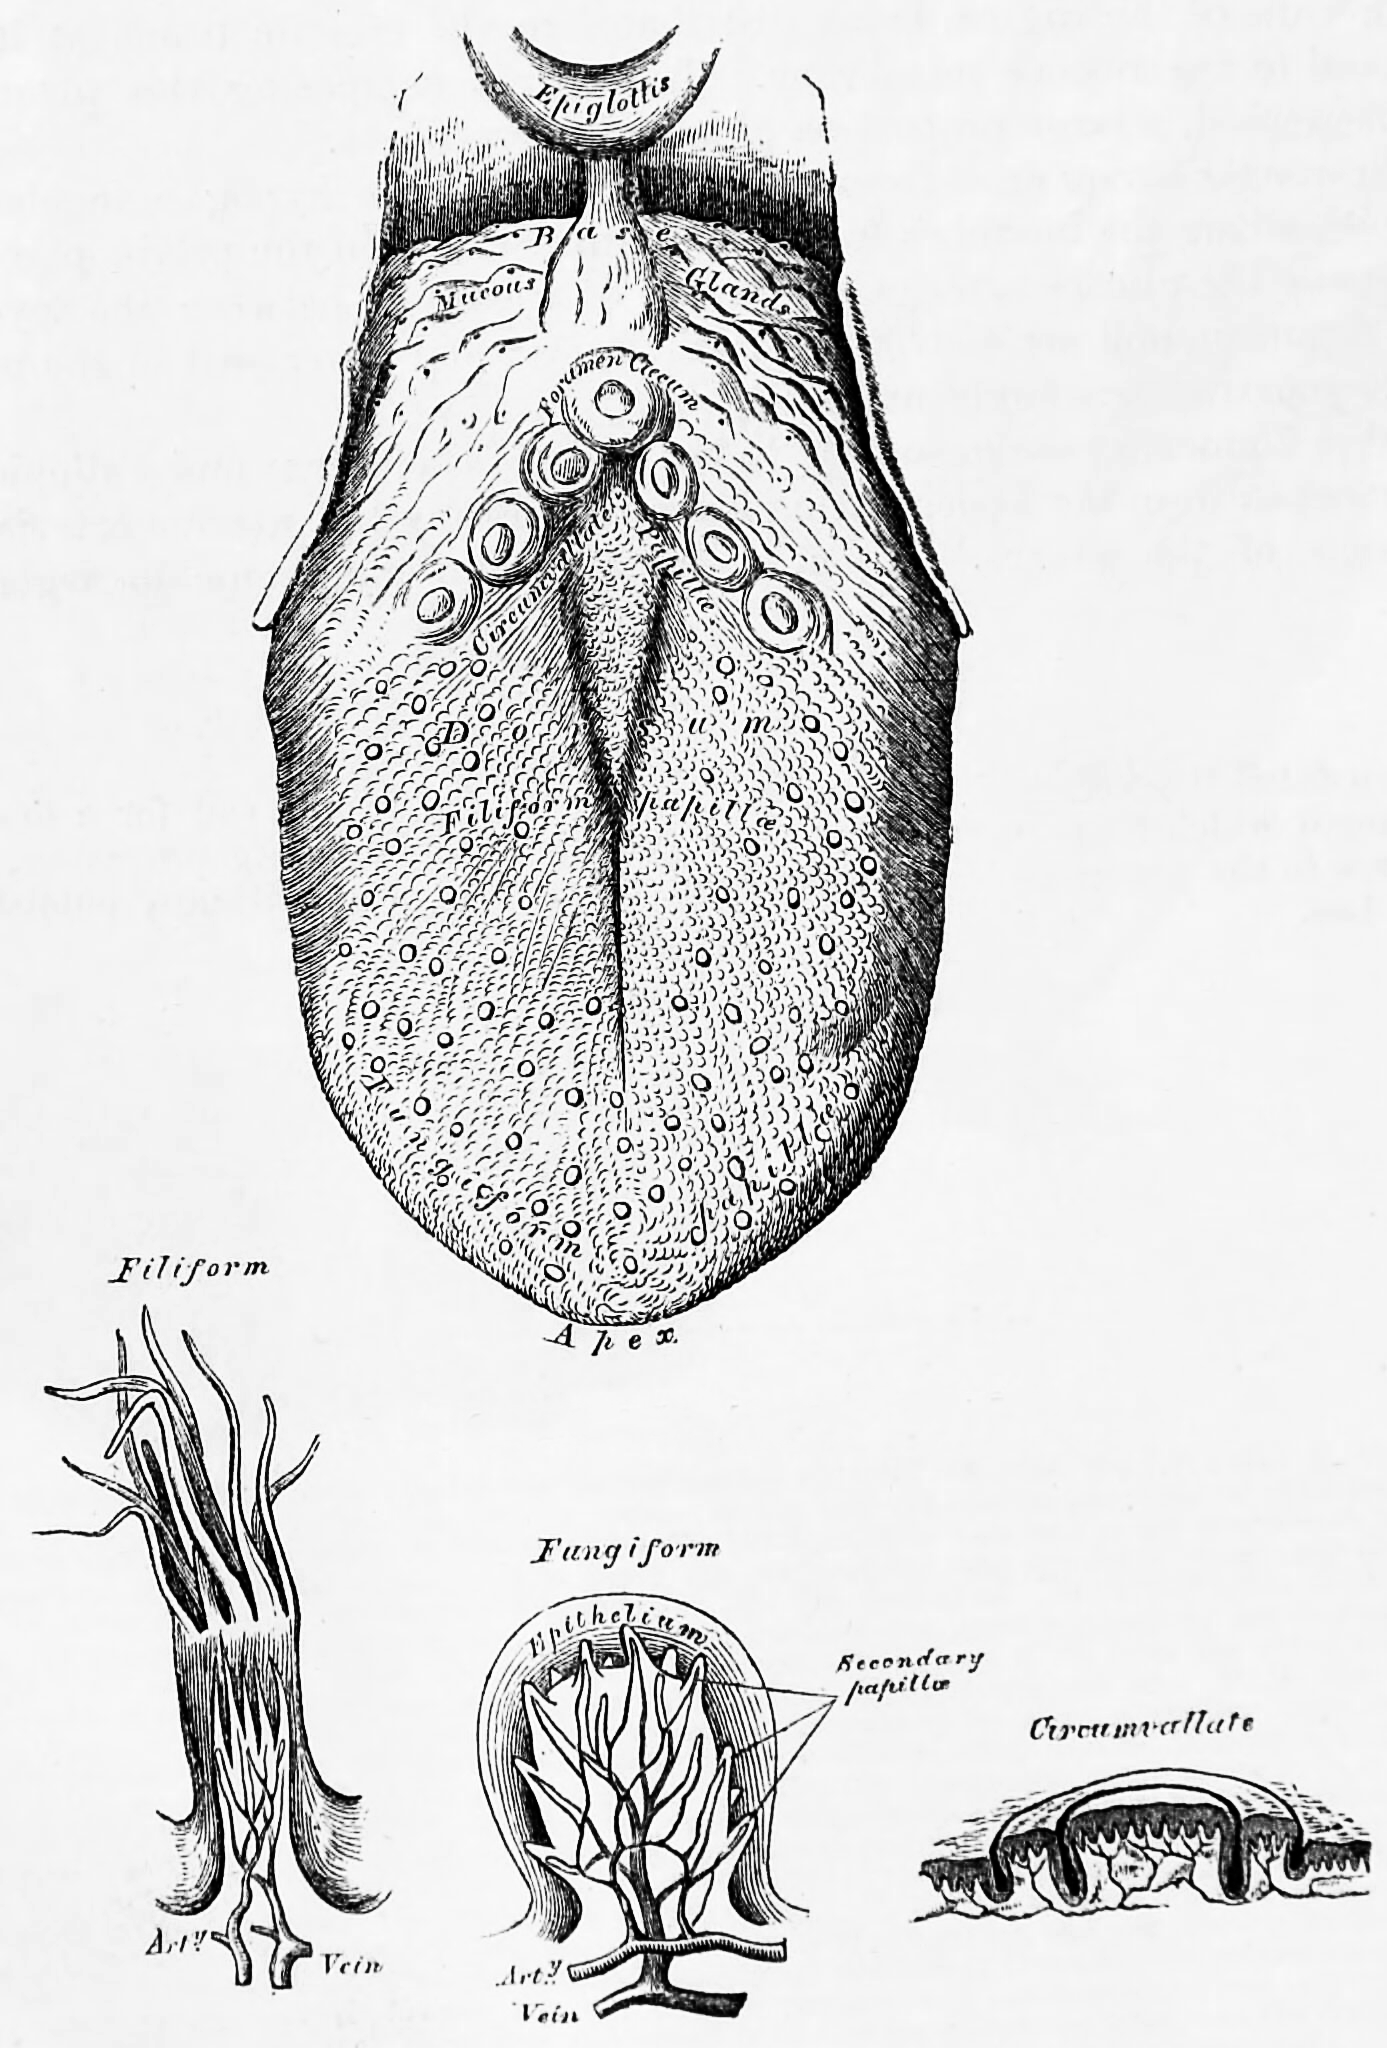
\includegraphics[width=0.7\linewidth]{./figures/sensation/tongue} 

}

\caption{The human tongue and three kinds of papillae magnified. Bottom left to right: filiform, fungiform and circumvallate papillae. From \href{https://wellcomelibrary.org/item/b21688692}{Gray, Henry: Anatomy Descriptive And Surgical. 7\textsuperscript{th} Edition, Longmans, Green, And Co., London, 1875}}\label{fig:tongue}
\end{figure}

Innervation of the tongue consists of motor fibers, special sensory fibers for taste, and general sensory fibers for sensation.

The tongue is covered with thousands of small bumps called papillae, which are visible to the naked eye. Within each papilla are hundreds of taste buds. The exception to this is the filiform papillae that do not contain taste buds. Each taste bud contains 50 to 100 taste receptor cells.



\begin{figure}

{\centering 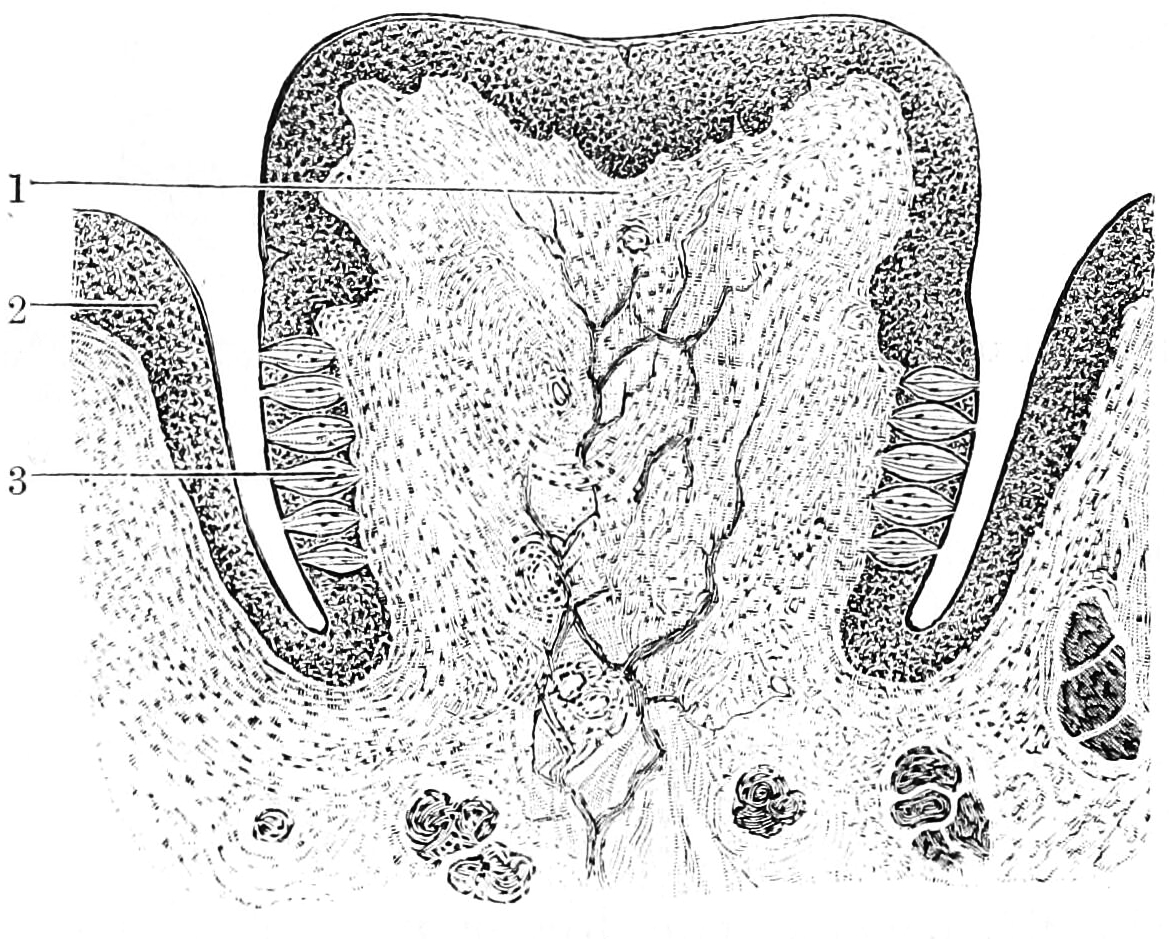
\includegraphics[width=0.7\linewidth]{./figures/sensation/CunninghamSection2Page770} 

}

\caption{Section through a papilla vallata of the human tongue. 1) Papilla. 2) Vallum. 3) Taste buds. From \href{https://wellcomelibrary.org/item/b21271070}{Textbook of anatomy. Section 2. The muscular system: the nervous system: the organs of sense and integument edited by D. J. Cunningham}}\label{fig:vallatepapilla}
\end{figure}

\hypertarget{the-five-basic-tastes}{%
\subsection{The Five Basic Tastes}\label{the-five-basic-tastes}}

The sensation of taste includes five established basic tastes: sweetness, sourness, saltiness, bitterness, and savoriness (also known as savory or umami). Taste buds are able to distinguish between different tastes through detecting interaction with different molecules or ions. Sweet, savoriness, and bitter tastes are triggered by the binding of molecules to G protein-coupled receptors on the cell membranes of taste buds. Saltiness and sourness are perceived when alkali metal or hydrogen ions enter taste buds, respectively.



\begin{figure}

{\centering 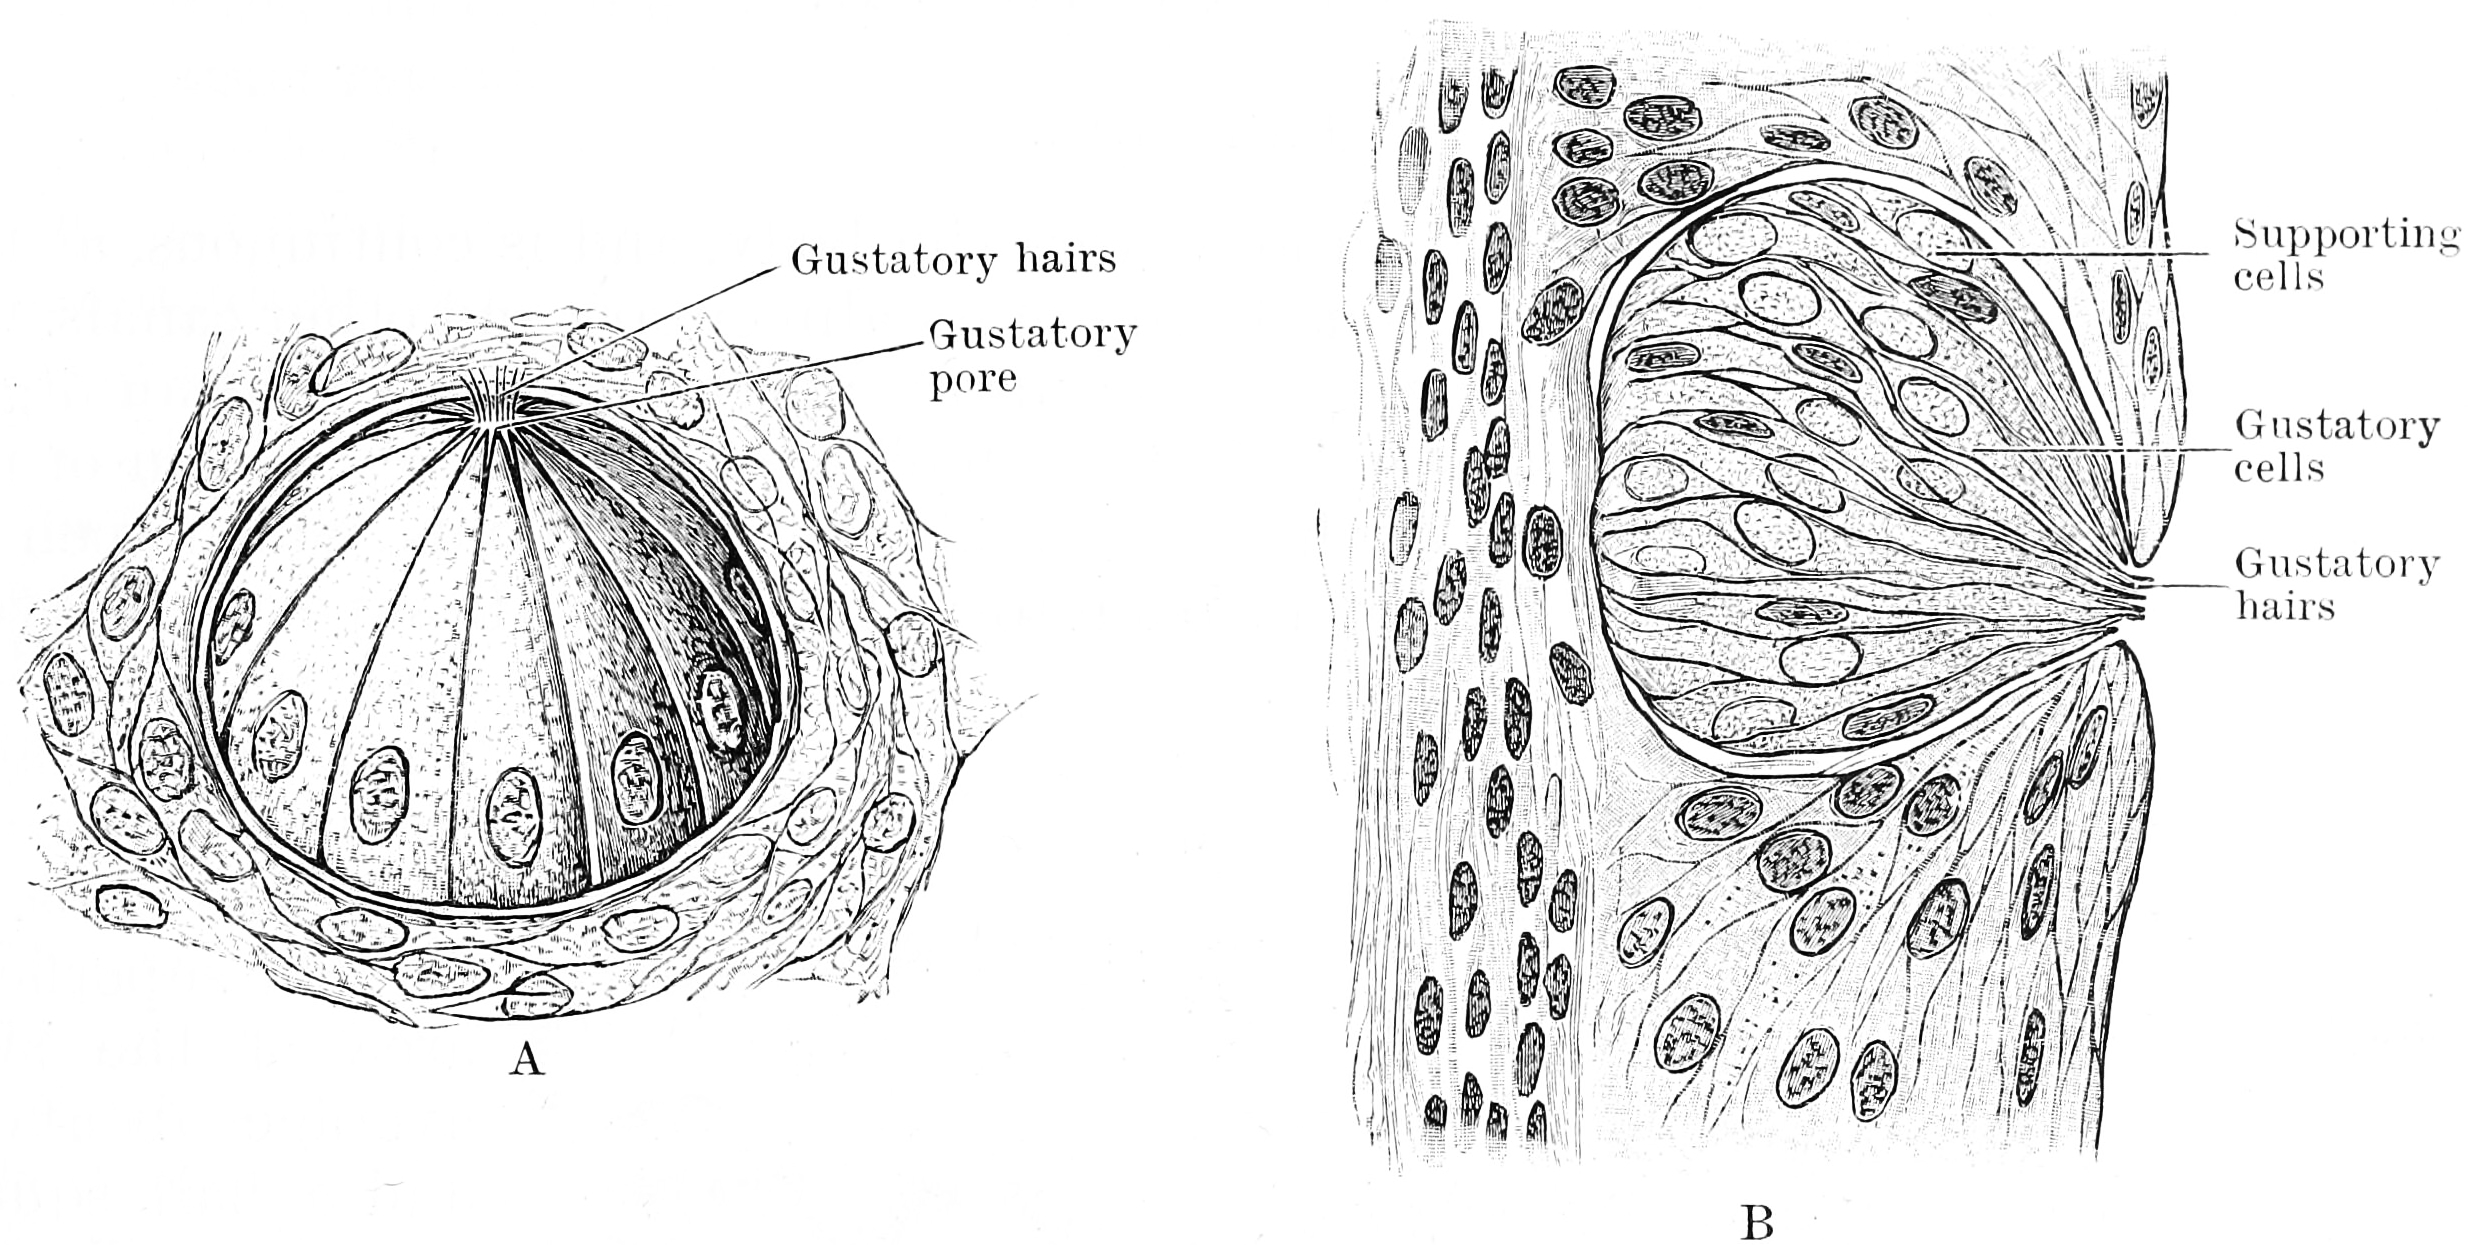
\includegraphics[width=0.7\linewidth]{./figures/sensation/CunninghamSection2Page771} 

}

\caption{A. Three quarter surface view of a taste bud from the papilla foliata of a rabbit (highly magnified). B. Vertical section of taste bud from the papilla foliata of a rabbit (highly magnified). From \href{https://wellcomelibrary.org/item/b21271070}{Textbook of anatomy. Section 2. The muscular system: the nervous system: the organs of sense and integument edited by D. J. Cunningham}}\label{fig:tastebuds}
\end{figure}



\begin{figure}

{\centering 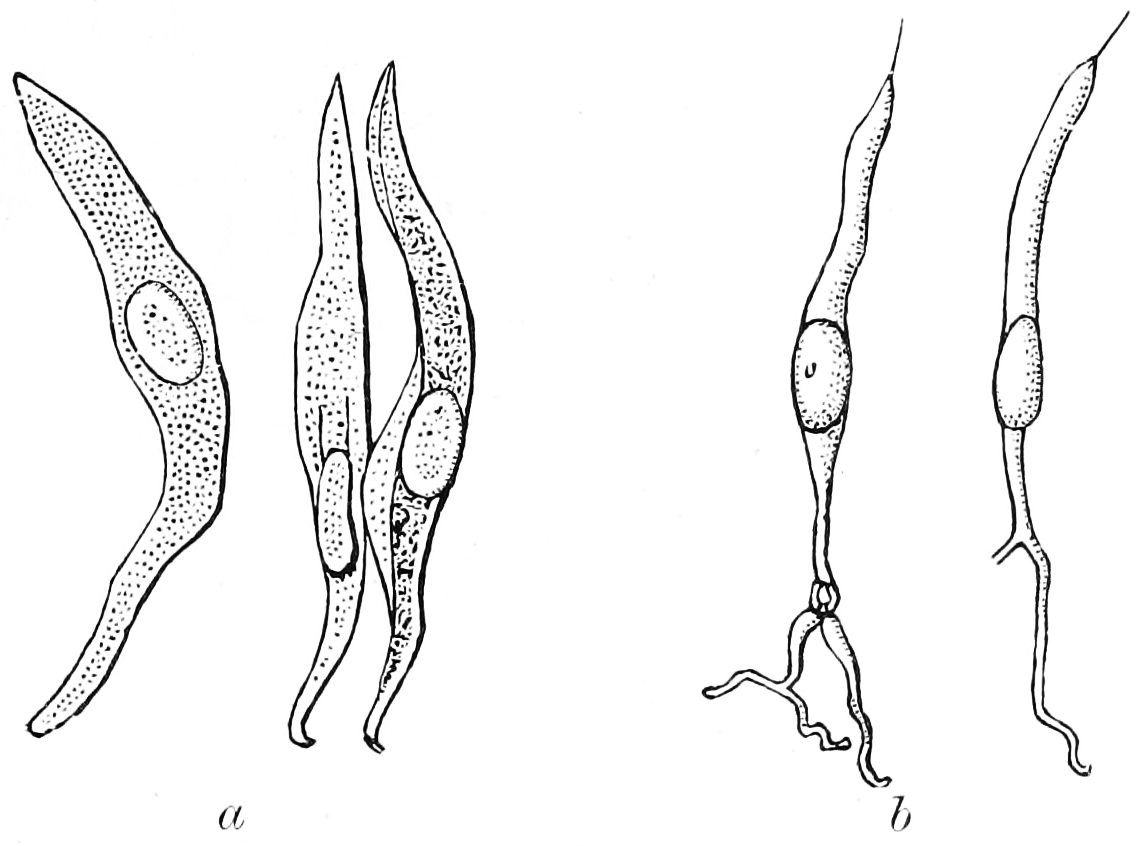
\includegraphics[width=0.7\linewidth]{./figures/sensation/CunninghamSection2Page771Cells} 

}

\caption{Isolated cells from taste bud of a rabbit. a, Supporting cells. b, Gustatory cells. From \href{https://wellcomelibrary.org/item/b21271070}{Textbook of anatomy. Section 2. The muscular system: the nervous system: the organs of sense and integument edited by D. J. Cunningham}}\label{fig:tastecells}
\end{figure}

The basic tastes contribute only partially to the sensation and flavor of food in the mouth---other factors include smell, detected by the olfactory epithelium of the nose; texture, detected through a variety of mechanoreceptors; temperature, detected by thermoreceptors; and ``coolness'' (such as of menthol) and ``hotness'' (pungency), through \href{https://en.wikipedia.org/wiki/Chemesthesis}{chemesthesis}.

As taste senses both harmful and beneficial things, all basic tastes are classified as either aversive or appetitive, depending upon the effect the things they sense have on our bodies. Sweetness helps to identify energy-rich foods, while bitterness serves as a warning sign of poisons.

Among humans, taste perception begins to fade around 50 years of age because of loss of tongue papillae and a general decrease in saliva production. Humans can also have distortion of tastes through dysgeusia. Not all mammals share the same taste senses: some rodents can taste starch (which humans cannot), cats cannot taste sweetness, and several other carnivores including hyenas, dolphins, and sea lions, have lost the ability to sense up to four of their ancestral five taste senses.

\hypertarget{sweetness}{%
\subsection{Sweetness}\label{sweetness}}

Sweetness, usually regarded as a pleasurable sensation, is produced by the presence of sugars and substances that mimic sugar. Sweetness may be connected to aldehydes and ketones, which contain a carbonyl group. Sweetness is detected by a variety of G protein coupled receptors (GPCR) coupled to the G protein gustducin found on the taste buds. At least two different variants of the ``sweetness receptors'' must be activated for the brain to register sweetness. Compounds the brain senses as sweet are compounds that can bind with varying bond strength to two different sweetness receptors. These receptors are T1R2+3 (heterodimer) and T1R3 (homodimer), which account for all sweet sensing in humans and animals. Taste detection thresholds for sweet substances are rated relative to sucrose, which has an index of 1. The average human detection threshold for sucrose is 10 millimoles per liter. For lactose it is 30 millimoles per liter, with a sweetness index of 0.3, and 5-nitro-2-propoxyaniline 0.002 millimoles per liter. ``Natural'' sweeteners such as saccharides activate the GPCR, which releases gustducin. The gustducin then activates the molecule adenylate cyclase, which catalyzes the production of the molecule cAMP, or adenosine 3', 5'-cyclic monophosphate. This molecule closes potassium ion channels, leading to depolarization and neurotransmitter release. Synthetic sweeteners such as saccharin activate different GPCRs and induce taste receptor cell depolarization by an alternate pathway.

\hypertarget{sourness}{%
\subsection{Sourness}\label{sourness}}

Sourness is the taste that detects acidity. The sourness of substances is rated relative to dilute hydrochloric acid, which has a sourness index of 1. By comparison, tartaric acid has a sourness index of 0.7, citric acid an index of 0.46, and carbonic acid an index of 0.06.

Sour taste is detected by a small subset of cells that are distributed across all taste buds in the tongue. Sour taste cells can be identified by expression of the protein PKD2L1, although this gene is not required for sour responses. There is evidence that the protons that are abundant in sour substances can directly enter the sour taste cells through apically located ion channels. In 2018, the proton-elective ion channel otopetrin 1 (Otop1) was implicated as the primary mediator of this proton influx. This transfer of positive charge into the cell can itself trigger an electrical response. It has also been proposed that weak acids such as acetic acid, which is not fully dissociated at physiological pH values, can penetrate taste cells and thereby elicit an electrical response. According to this mechanism, intracellular hydrogen ions inhibit potassium channels, which normally function to hyperpolarize the cell. By a combination of direct intake of hydrogen ions (which itself depolarizes the cell) and the inhibition of the hyperpolarizing channel, sourness causes the taste cell to fire action potentials and release neurotransmitter.

\hypertarget{saltiness}{%
\subsection{Saltiness}\label{saltiness}}

The simplest receptor found in the mouth is the sodium chloride (salt) receptor. Saltiness is a taste produced primarily by the presence of sodium ions. Other ions of the alkali metals group also taste salty, but the further from sodium, the less salty the sensation is. A sodium channel in the taste cell membrane allows sodium cations to enter the cell. This on its own depolarizes the cell, and opens voltage-dependent calcium channels, flooding the cell with positive calcium ions and leading to neurotransmitter release. This sodium channel is known as an epithelial sodium channel (ENaC) and is composed of three subunits. An ENaC can be blocked by the drug amiloride in many mammals, especially rats. The sensitivity of the salt taste to amiloride in humans, however, is much less pronounced, leading to conjecture that there may be additional receptor proteins besides ENaC to be discovered.

The size of lithium and potassium ions most closely resemble those of sodium, and thus the saltiness is most similar. In contrast, rubidium and caesium ions are far larger, so their salty taste differs accordingly. The saltiness of substances is rated relative to sodium chloride (NaCl), which has an index of 1. Potassium, as potassium chloride (KCl), is the principal ingredient in salt substitutes and has a saltiness index of 0.6.

Other monovalent cations, e.g.~ammonium (NH\textsubscript{4}\textsuperscript{+}), and divalent cations of the alkali earth metal group of the periodic table, e.g.~calcium (Ca\textsuperscript{2+}), ions generally elicit a bitter rather than a salty taste even though they, too, can pass directly through ion channels in the tongue, generating an action potential.

\hypertarget{bitterness}{%
\subsection{Bitterness}\label{bitterness}}

Bitterness is one of the most sensitive of the tastes, and many perceive it as unpleasant, sharp, or disagreeable, but it is sometimes desirable and intentionally added via various bittering agents. Common bitter foods and beverages include coffee, unsweetened cocoa, South American mate, coca tea, bitter gourd, uncured olives, citrus peel, many plants in the family \emph{Brassicaceae}, dandelion greens, horehound, wild chicory, and escarole. The ethanol in alcoholic beverages tastes bitter, as do the additional bitter ingredients found in some alcoholic beverages including hops in beer and \emph{Gentiana} in bitters. Quinine is also known for its bitter taste and is found in tonic water.

Bitterness is of interest to those who study evolution, as well as various health researchers since a large number of natural bitter compounds are known to be toxic. The ability to detect bitter-tasting, toxic compounds at low thresholds is considered to provide an important protective function. Plant leaves often contain toxic compounds, and among leaf-eating primates there is a tendency to prefer immature leaves, which tend to be higher in protein and lower in fiber and poisons than mature leaves. Amongst humans, various food processing techniques are used worldwide to detoxify otherwise inedible foods and make them palatable. Furthermore, the use of fire, changes in diet, and avoidance of toxins has led to neutral evolution in human bitter sensitivity. This has allowed several loss of function mutations that has led to a reduced sensory capacity towards bitterness in humans when compared to other species.

The threshold for stimulation of bitter taste by quinine averages a concentration of 8 μM (8 micromolar). The taste thresholds of other bitter substances are rated relative to quinine, which is thus given a reference index of 1. For example, brucine has an index of 11, is thus perceived as intensely more bitter than quinine, and is detected at a much lower solution threshold. The most bitter natural substance is amarogentin a compound present in the roots of the plant \emph{Gentiana lutea} and the most bitter substance known is the synthetic chemical denatonium, which has an index of 1,000. It is used as an aversive agent (a bitterant) that is added to toxic substances to prevent accidental ingestion.

Research has shown that TAS2Rs (taste receptors, type 2, also known as T2Rs) such as TAS2R38 coupled to the G protein gustducin are responsible for the human ability to taste bitter substances. The TAS2R family in humans is thought to comprise about 25 different taste receptors, some of which can recognize a wide variety of bitter-tasting compounds. Over 670 bitter-tasting compounds have been identified, on a bitter database, of which over 200 have been assigned to one or more specific receptors. Researchers use two synthetic substances, phenylthiocarbamide (PTC) and 6-n-propylthiouracil (PROP) to study the genetics of bitter perception. These two substances taste bitter to some people, but are virtually tasteless to others. Among the tasters, some are so-called ``supertasters'' to whom PTC and PROP are extremely bitter. The variation in sensitivity is determined by two common alleles at the TAS2R38 locus.

\hypertarget{savoriness-umami}{%
\subsection{Savoriness (Umami)}\label{savoriness-umami}}

Savory, or savoriness is an appetitive taste and is occasionally described by its Japanese name, umami or ``meaty''.

\hypertarget{the-taste-receptors}{%
\subsection{The Taste Receptors}\label{the-taste-receptors}}

There are four types taste receptors. When food or other substances enter the mouth, molecules interact with saliva and are bound to taste receptors in the oral cavity and other locations. Molecules which give a sensation of taste are considered ``sapid''.

Taste receptors are divided into two families:

\begin{itemize}
\tightlist
\item
  Type 1, sweet: TAS1R2+TAS1R3; umami: TAS1R1+TAS1R3
\item
  Type 2, bitter: TAS2R
\end{itemize}

The standard bitter, sweet, or umami taste receptors are G protein-coupled receptors with seven transmembrane domains. Ligand binding at the taste receptors activate second messenger cascades to depolarize the taste cell. Gustducin is the most common taste Gα subunit, having a major role in TAS2R bitter taste reception. Gustducin is a homologue for transducin, a G-protein involved in vision transduction. Additionally, taste receptors share the use of the TRPM5 ion channel, as well as a phospholipase PLCβ2.

The TAS1R1+TAS1R3 heterodimer receptor functions as an umami receptor, responding to L-amino acid binding, especially L-glutamate. The umami taste is most frequently associated with the food additive monosodium glutamate (MSG) and can be enhanced through the binding of inosine monophosphate (IMP) and guanosine monophosphate (GMP) molecules. TAS1R1+3 expressing cells are found mostly in the fungiform papillae at the tip and edges of the tongue and palate taste receptor cells in the roof of the mouth. These cells are shown to synapse upon the chorda tympani nerves to send their signals to the brain, although some activation of the glossopharyngeal nerve has been found.

Alternative candidate umami taste receptors include splice variants of metabotropic glutamate receptors, mGluR4 and mGluR1, and the N-methyl-D-aspartate type glutamate ion channel receptor.

The TAS1R2+TAS1R3 heterodimer receptor functions as the sweet receptor by binding to a wide variety of sugars and sugar substitutes. TAS1R2+3 expressing cells are found in circumvallate papillae and foliate papillae near the back of the tongue and palate taste receptor cells in the roof of the mouth. These cells are shown to synapse upon the chorda tympani and glossopharyngeal nerves to send their signals to the brain. The TAS1R3 homodimer also functions as a sweet receptor in much the same way as TAS1R2+3 but has decreased sensitivity to sweet substances. Natural sugars are more easily detected by the TAS1R3 receptor than sugar substitutes. This may help explain why sugar and artificial sweeteners have different tastes. Genetic polymorphisms in TAS1R3 partly explain the difference in sweet taste perception and sugar consumption between people of African American ancestry and people of European and Asian ancestries.

The TAS2R proteins function as bitter taste receptors. There are 43 human TAS2R genes, each of which (excluding the five pseudogenes) lacks introns and codes for a GPCR protein. These proteins, as opposed to TAS1R proteins, have short extracellular domains and are located in circumvallate papillae, palate, foliate papillae, and epiglottis taste buds, with reduced expression in fungiform papillae. Though it is certain that multiple TAS2Rs are expressed in one taste receptor cell, it is still debated whether mammals can distinguish between the tastes of different bitter ligands. Some overlap must occur, however, as there are far more bitter compounds than there are TAS2R genes. Common bitter ligands include cycloheximide, denatonium, PROP (6-n-propyl-2-thiouracil), PTC (phenylthiocarbamide), and β-glucopyranosides.

Signal transduction of bitter stimuli is accomplished via the α-subunit of gustducin. This G protein subunit activates a taste phosphodiesterase and decreases cyclic nucleotide levels. Further steps in the transduction pathway are still unknown. The βγ-subunit of gustducin also mediates taste by activating IP3 (inositol triphosphate) and DAG (diglyceride). These second messengers may open gated ion channels or may cause release of internal calcium. Though all TAS2Rs are located in gustducin-containing cells, knockout of gustducin does not completely abolish sensitivity to bitter compounds, suggesting a redundant mechanism for bitter tasting (unsurprising given that a bitter taste generally signals the presence of a toxin). One proposed mechanism for gustducin-independent bitter tasting is via ion channel interaction by specific bitter ligands, similar to the ion channel interaction which occurs in the tasting of sour and salty stimuli.

One of the best-researched TAS2R proteins is TAS2R38, which contributes to the tasting of both PROP and PTC. It is the first taste receptor whose polymorphisms are shown to be responsible for differences in taste perception. Current studies are focused on determining other such taste phenotype-determining polymorphisms. More recent studies show that genetic polymorphisms in other bitter taste receptor genes influence bitter taste perception of caffeine, quinine and denatonium benzoate.

Historically it was thought that the sour taste was produced solely when free hydrogen ions (H\textsuperscript{+}) directly depolarised taste receptors. However, specific receptors for sour taste with other methods of action are now being proposed. HCN1 and HCN4 (HCN channels) were two such proposals; both of these receptors are cyclic nucleotide-gated channels. The two ion channels suggested to contribute to sour taste are ACCN1 and TASK-1.

Various receptors have also been proposed for salty tastes, along with the possible taste detection of lipids, complex carbohydrates, and water. Evidence for these receptors is, however, shaky at best, and is often unconvincing in mammal studies. For example, the proposed ENaC receptor for sodium detection can only be shown to contribute to sodium taste in Drosophilia.

Visual, olfactive, ``sapictive'' (the perception of tastes), trigeminal (hot, cool), mechanical, all contribute to the perception of taste. Of these, transient receptor potential cation channel subfamily V member 1 (TRPV1) vanilloid receptors are responsible for the perception of heat from some molecules such as capsaicin, and a CMR1 receptor is responsible for the perception of cold from molecules such as menthol, eucalyptol, and icilin.

\hypertarget{the-gustatory-cortex}{%
\subsection{The Gustatory Cortex}\label{the-gustatory-cortex}}

The primary gustatory cortex is a brain structure responsible for the perception of taste. It consists of two substructures: the anterior insula on the insular lobe and the frontal operculum on the inferior frontal gyrus of the frontal lobe. Because of its composition the primary gustatory cortex is sometimes referred to in literature as the AI/FO(Anterior Insula/Frontal Operculum). By using extracellular unit recording techniques, scientists have elucidated that neurons in the AI/FO respond to sweetness, saltiness, bitterness, and sourness, and they code the intensity of the taste stimulus.

Like the olfactory system, the taste system is defined by its specialized peripheral receptors and central pathways that relay and process taste information. Peripheral taste receptors are found on the upper surface of the tongue, soft palate, pharynx, and the upper part of the esophagus. Taste cells synapse with primary sensory axons that run in the chorda tympani and greater superficial petrosal branches of the facial nerve (cranial nerve VII), the lingual branch of the glossopharyngeal nerve (cranial nerve IX), and the superior laryngeal branch of the vagus nerve (Cranial nerve X) to innervate the taste buds in the tongue, palate, epiglottis, and esophagus respectively. The central axons of these primary sensory neurons in the respective cranial nerve ganglia project to rostral and lateral regions of the nucleus of the solitary tract in the medulla, which is also known as the gustatory nucleus of the solitary tract complex. Axons from the rostral (gustatory) part of the solitary nucleus project to the ventral posterior complex of the thalamus, where they terminate in the medial half of the ventral posterior medial nucleus. This nucleus projects in turn to several regions of the neocortex which includes the gustatory cortex (the frontal operculum and the insula), which becomes activated when the subject is consuming and experiencing taste.


